%%%%%%%%%%%%%%%%%%%%%%%%%%%%%%%%%%%%%%%%
% datoteka diploma-vzorec.tex
%
% vzorčna datoteka za pisanje diplomskega dela v formatu LaTeX
% na UL Fakulteti za računalništvo in informatiko
%
% vkup spravil Gašper Fijavž, december 2010
%
% (za zgodovino verzij glej originalno predlogo)
% verzija junij 2018 (Polona Oblak, IŠRM predloga)


\documentclass[a4paper, 12pt]{book}
%\documentclass[a4paper, 12pt, draft]{book}  Nalogo preverite tudi z opcijo draft, ki vam bo pokazala, katere vrstice so predolge!



\usepackage[utf8x]{inputenc}   % omogoča uporabo slovenskih črk kodiranih v formatu UTF-8
\usepackage[slovene,english]{babel}    % naloži, med drugim, slovenske delilne vzorce
\usepackage[pdftex]{graphicx}  % omogoča vlaganje slik različnih formatov
\usepackage{fancyhdr}          % poskrbi, na primer, za glave strani
\usepackage{amssymb}           % dodatni simboli
\usepackage{amsmath}           % eqref, npr.
%\usepackage{hyperxmp}
\usepackage[hyphens]{url}  % dodal Solina
\usepackage{comment}       % dodal Solina
\usepackage{tikz}
\usetikzlibrary{arrows.meta,positioning}
\usepackage{booktabs}      % lepe tabele (za povzetek metrik)
\usepackage[pdftex, colorlinks=true,
						citecolor=black, filecolor=black,
						linkcolor=black, urlcolor=black,
						pagebackref=false,
						pdfproducer={LaTeX}, pdfcreator={LaTeX}, hidelinks]{hyperref}

\usepackage{color}       % dodal Solina
\usepackage{soul}       % dodal Solina
\usepackage{float}       % za [H]
\usepackage{subcaption}  % za subfigure

% oznaka problema: \prob{23}{1} -> F_{23}I_{1}  (uporabi v matematicnem nacinu)
\newcommand{\prob}[2]{F_{#1}I_{#2}}

%%%%%%%%%%%%%%%%%%%%%%%%%%%%%%%%%%%%%%%%
%	DIPLOMA INFO
%%%%%%%%%%%%%%%%%%%%%%%%%%%%%%%%%%%%%%%%
\newcommand{\ttitle}{Analiza in vizualizacija algoritmov za optimizacijo prek iskalnih trajektorij}
\newcommand{\ttitleEn}{Analysis and Visualization of Optimization Algorithms via Search Trajectories}
\newcommand{\tsubject}{\ttitle}
\newcommand{\tsubjectEn}{\ttitleEn}
\newcommand{\tauthor}{Timon Bubnič}
\newcommand{\tkeywords}{metahevristike, iskalne trajektorije, mere podobnosti, gručenje, BBOB, vizualizacija}
\newcommand{\tkeywordsEn}{metaheuristics, search trajectories, similarity measures, clustering, BBOB, visualization}


%%%%%%%%%%%%%%%%%%%%%%%%%%%%%%%%%%%%%%%%
%	HYPERREF SETUP
%%%%%%%%%%%%%%%%%%%%%%%%%%%%%%%%%%%%%%%%
\hypersetup{pdftitle={\ttitle}}
\hypersetup{pdfsubject=\ttitleEn}
\hypersetup{pdfauthor={\tauthor, tb58222@student.uni-lj.si}}
\hypersetup{pdfkeywords=\tkeywordsEn}


%%%%%%%%%%%%%%%%%%%%%%%%%%%%%%%%%%%%%%%%
% postavitev strani
%%%%%%%%%%%%%%%%%%%%%%%%%%%%%%%%%%%%%%%%

\addtolength{\marginparwidth}{-20pt} % robovi za tisk
\addtolength{\oddsidemargin}{40pt}
\addtolength{\evensidemargin}{-40pt}

\renewcommand{\baselinestretch}{1.3} % ustrezen razmik med vrsticami
\setlength{\headheight}{15pt}        % potreben prostor na vrhu
\renewcommand{\chaptermark}[1]%
{\markboth{\MakeUppercase{\thechapter.\ #1}}{}} \renewcommand{\sectionmark}[1]%
{\markright{\MakeUppercase{\thesection.\ #1}}} \renewcommand{\headrulewidth}{0.5pt} \renewcommand{\footrulewidth}{0pt}
\fancyhf{}
\fancyhead[LE,RO]{\sl \thepage}
\fancyhead[RE]{\sc \tauthor}              % dodal Solina
\fancyhead[LO]{\sc Diplomska naloga}     % dodal Solina


\newcommand{\BibTeX}{{\sc Bib}\TeX}

%%%%%%%%%%%%%%%%%%%%%%%%%%%%%%%%%%%%%%%%
% naslovi
%%%%%%%%%%%%%%%%%%%%%%%%%%%%%%%%%%%%%%%%


\newcommand{\autfont}{\Large}
\newcommand{\titfont}{\LARGE\bf}
\newcommand{\clearemptydoublepage}{\newpage{\pagestyle{empty}\cleardoublepage}}
\setcounter{tocdepth}{1}	      % globina kazala

%%%%%%%%%%%%%%%%%%%%%%%%%%%%%%%%%%%%%%%%
% konstrukti
%%%%%%%%%%%%%%%%%%%%%%%%%%%%%%%%%%%%%%%%
\newtheorem{izrek}{Izrek}[chapter]
\newtheorem{definicija}[izrek]{Definicija}
\newtheorem{trditev}{Trditev}[izrek]
\newtheorem{lema}[izrek]{Lema}
\newenvironment{dokaz}{\emph{Dokaz.}\ }{\hspace{\fill}{$\Box$}}

\begin{document}
\selectlanguage{slovene}
\frontmatter
\setcounter{page}{1}
\renewcommand{\thepage}{}
\newcommand{\sn}[1]{"`#1"'}

%%%%%%%%%%%%%%%%%%%%%%%%%%%%%%%%%%%%%%%%
% naslovnica
 \thispagestyle{empty}%
   \begin{center}
    {\large\sc Univerza v Ljubljani\\%
      Fakulteta za računalništvo in informatiko\\%
      Fakulteta za matematiko in fiziko}%
    \vskip 10em%
    {\autfont \tauthor\par}%
    {\titfont \ttitle \par}%
    {\vskip 3em \textsc{DIPLOMSKO DELO\\[5mm]
    INTERDISCIPLINARNI UNIVERZITETNI\\ ŠTUDIJSKI PROGRAM PRVE STOPNJE\\ RAČUNALNIŠTVO IN MATEMATIKA}\par}%
    \vfill\null%
    {\large \textsc{Mentor}: doc.\ dr.  Janoš Vidali\par}%

    {\vskip 2em \large Ljubljana, 2026 \par}%
\end{center}

%%%%%%%%%%%%%%%%%%%%%%%%%%%%%%%%%%%%%%%%
% copyright stran
\thispagestyle{empty}
\vspace*{8cm}

\noindent
{\sc Copyright}.
Rezultati diplomske naloge so intelektualna lastnina avtorja in Fakultete za računalništvo in informatiko Univerze v Ljubljani.
Za objavo in koriščenje rezultatov diplomske naloge je potrebno pisno privoljenje avtorja, Fakultete za računalništvo in informatiko ter mentorja.

\begin{center}
\mbox{}\vfill
\emph{Besedilo je oblikovano z urejevalnikom besedil \LaTeX.}
\end{center}
\clearemptydoublepage

%%%%%%%%%%%%%%%%%%%%%%%%%%%%%%%%%%%%%%%%
% stran 3 med uvodnimi listi
\thispagestyle{empty}
\vspace*{4cm}

\noindent
Fakulteta za računalništvo in informatiko izdaja naslednjo nalogo:
\medskip
\begin{tabbing}
\hspace{32mm}\= \hspace{6cm} \= \kill
Tematika naloge:
\end{tabbing}

\vspace{15mm}
\vspace{2cm}
\clearemptydoublepage

% zahvala
\thispagestyle{empty}\mbox{}\vfill\null\it%
\noindent
Zahvalil bi se rad svoji družini za podporo in potrpežljivost skozi študij. Prav tako bi se rad zahvalil tudi mentorju doc. dr. Janošu Vidaliju in somentorici dr. Gjorgjini Cenikj za hitre odgovore in pomoč pri izdelavi diplome. Hvala tudi prijateljem in sošolcem, ki so mi čez študij stali ob strani. 

\rm\normalfont
\clearemptydoublepage

%%%%%%%%%%%%%%%%%%%%%%%%%%%%%%%%%%%%%%%%
% kazalo
\pagestyle{empty}
\def\thepage{}%
\tableofcontents{}
\clearemptydoublepage

%%%%%%%%%%%%%%%%%%%%%%%%%%%%%%%%%%%%%%%%
% seznam kratic
\chapter*{Seznam uporabljenih kratic}

\noindent\begin{tabular}{p{0.1\textwidth}|p{.4\textwidth}|p{.4\textwidth}}
  {\bf kratica} & {\bf angleško}                             & {\bf slovensko} \\ \hline
  {BBOB} & {Black-box optimization benchmarking} & {Vrednotenje optimizacije črne škatle} \\ \hline
  {MHA} & {Metaheuristic algorithm} & {Metahevristični algoritem}
\end{tabular}
\clearemptydoublepage

%%%%%%%%%%%%%%%%%%%%%%%%%%%%%%%%%%%%%%%%
% povzetek
\addcontentsline{toc}{chapter}{Povzetek}
\chapter*{Povzetek}

\noindent\textbf{Naslov:} \ttitle
\bigskip

\noindent\textbf{Avtor:} \tauthor
\bigskip

\noindent
Metahevristične optimizacijske algoritme praviloma primerjamo po kakovosti
rešitve, ki jo dosežejo, kar pa ne pove ničesar o tem, kako so do nje prišli.
V tem delu predstavimo nabor šestih komplementarnih mer podobnosti, ki
vedenje dveh algoritmov primerjajo neposredno iz njunih iskalnih trajektorij.
Pet mer je izvirnih, kosinusno razdaljo prevzamemo iz predhodnega dela. Mere
ovrednotimo na 28 algoritmih knjižnice mealpy, pognanih na primerjalnem
naboru BBOB v dimenzijah 2, 5 in 10. Spearmanova korelacija pokaže, da so
mere med seboj večinoma šibko povezane, zato vsaka prispeva svoj vidik
vedenja. Pokažemo tudi, da se z naraščajočo dimenzijo iskalno vedenje
algoritma vse bolj razklopi od kakovosti končne rešitve.

\bigskip

\noindent\textbf{Ključne besede:} \tkeywords.
\clearemptydoublepage

\selectlanguage{english}
\addcontentsline{toc}{chapter}{Abstract}
\chapter*{Abstract}

\noindent\textbf{Title:} \ttitleEn
\bigskip

\noindent\textbf{Author:} \tauthor
\bigskip

\noindent
Metaheuristic optimization algorithms are usually compared by the quality of
the solution they reach, which says nothing about how they searched for it.
This work presents a set of six complementary similarity measures that
compare the behaviour of two algorithms directly from their search
trajectories. Five of the measures are original, while the cosine distance is
adopted from earlier work. We evaluate the measures on 28 algorithms from the
mealpy library, run on the BBOB benchmark suite in dimensions 2, 5 and 10.
Spearman correlation shows that the measures are largely only weakly related,
so each contributes a distinct view of behaviour. We further show that with
increasing dimension, search behaviour becomes progressively decoupled from
final solution quality.

\bigskip

\noindent\textbf{Keywords:} \tkeywordsEn.
\selectlanguage{slovene}
\clearemptydoublepage

\mainmatter
\setcounter{page}{1}
\pagestyle{fancy}

\chapter{Uvod}

Optimizacijski problemi, pri katerih kriterijske funkcije ne poznamo v
analitični obliki in jo lahko le vrednotimo v posameznih točkah, so v praksi
pogosti. Za njihovo reševanje so se uveljavile \emph{metahevristike}, splošne
iterativne metode iskanja, ki s kombinacijo naključnosti in hevrističnih
pravil iščejo kakovostne približne rešitve. Njihovo število hitro narašča;
knjižnica mealpy~\cite{van2023mealpy} jih ponuja več kot dvesto.

Uspešnost teh metod praviloma primerjamo po kakovosti rešitve, ki jo
algoritem doseže v danem proračunu vrednotenj. Tak način je preprost in
ponovljiv, pove pa le, \emph{kaj} je algoritem našel, ne pa, \emph{kako} je
do tega prišel. Dva algoritma lahko na istem problemu dosežeta praktično
enako kakovostno rešitev po povsem različnih poteh.

Da merjenje uspešnosti ne zadošča, nakazuje tudi izrek o neobstoju
brezplačnega kosila~\cite{585893}: povprečna uspešnost vseh algoritmov,
povprečena čez vse kriterijske funkcije, je enaka. Univerzalno najboljšega
algoritma torej ni in vprašanje, kateri je najboljši, je smiselno le ob
navedbi razreda problemov. Ostane vprašanje, po čem se algoritmi sploh
razlikujejo, odgovor nanj pa je vezan na njihovo vedenje med iskanjem. To je
toliko bolj aktualno, ker se ob naraščanju števila objavljenih metahevristik
poraja dvom o njihovi dejanski novosti. Nekatere se namreč kljub drugačni izvorni
metafori po iskalnem vedenju bistveno ne razlikujejo od že obstoječih.

Prispevek tega dela je \emph{nabor komplementarnih mer podobnosti}, od
katerih vsaka za dani par algoritmov na istem problemu in zagonu vrne eno
samo številsko vrednost. Vsaka zajame drugačen vidik iskanja: kako široko je
algoritem razporejal populacijo, katere regije prostora je zasedal in kdaj,
kako je uravnaval razmerje med raziskovanjem in izkoriščanjem ter kje in kako
dobro je pristal. Ker noben vidik sam ne opiše vedenja v celoti, mere niso
alternative, med katerimi bi bilo treba izbrati eno, temveč nabor, ki šele
skupaj da uporaben vpogled. Da je tak nabor smiseln, s korelacijsko analizo
pokažemo, da se mere med seboj ne podvajajo.

Poudariti velja, česa delo ne počne. Ne odgovarja na vprašanje, katera dva
algoritma sta si najbolj podobna, in ne razvršča algoritmov po uspešnosti.
Nabor 28 metahevristik, na katerem mere preizkusimo, je demonstracijski
vzorec, ne popis obstoječih metod; ugotovitve o posameznih algoritmih v
poglavju~\ref{ch:rezultati} so zato ponazoritev uporabnosti mer in ne
dokončne trditve o teh algoritmih.

Mere temeljijo na \emph{populacijskih trajektorijah}, torej na položajih vseh
agentov skozi vse iteracije zagona, ne le na najboljši najdeni rešitvi.
Zajamemo jih na standardnem primerjalnem naboru BBOB~\cite{hansen2021coco} in
jih z gručenjem pretvorimo v jedrnatejšo predstavitev, iz katere mere
izračunamo. Gručenje in kosinusno mero nad to predstavitvijo prevzamemo iz
predhodnega dela~\cite{clustopt2025, cenikj2025searchbehavior}, preostalih
pet mer je izvirnih. Vizualizacija pri tem ni samostojen prispevek, temveč
sredstvo, s katerim rezultate mer beremo in razlagamo.

Delo je razdeljeno takole. Poglavje 2 uvede osnovne pojme optimizacije črne
škatle in metahevristik, opredeli metriko in psevdometriko ter predstavi
primerjalni nabor BBOB. Poglavje 3 opiše izvedbo optimizacijskih zagonov,
zajem trajektorij in postopek gručenja. Poglavje~\ref{ch:metrike} formalno
definira šest mer podobnosti in razmeji, kaj je prevzeto in kaj izvirno.
Poglavje~\ref{ch:rezultati} mere uporabi na naboru 28 algoritmov in pokaže,
kaj o njihovem vedenju razkrijejo. Poglavje~\ref{ch:zakljuck} povzame
ugotovitve, navede omejitve dela in nakaže smeri nadaljnjega razvoja.


\chapter{Ozadje}

V tem poglavju opišemo osnove optimizacije, in sicer pojme kriterijske funkcije, globalnega in lokalnega minimuma, metrike in psevdometrike, pojem črne škatle ter uvod v teorijo metahevristik. V razdelku~\ref{sec:bbob} predstavimo tudi ogrodje za testiranje in primerjavo optimizacijskih algoritmov ter ponazorimo krajine problemov, na katerih bomo izvajali poskuse.

\section{Optimizacija in metahevristike}

Optimizacijski problem je naloga iskanja elementa dane množice, ki je glede
na izbrano merilo najboljši. To merilo podamo s \emph{kriterijsko funkcijo}
\[
    f \colon \Omega \to \mathbb{R},
\]
kjer je $\Omega \subseteq \mathbb{R}^n$ \emph{dopustna množica}, torej množica
vseh dopustnih rešitev, $n$ pa dimenzija iskalnega prostora. Element
$x \in \Omega$ imenujemo dopustna rešitev, vrednost $f(x)$ pa vrednost kriterijske funkcije.

Pri \emph{minimizaciji} iščemo dopustno rešitev z najmanjšo vrednostjo kriterijske funkcije, torej
\[
    x^{*} = \arg\min_{x \in \Omega} f(x),
\]
pri \emph{maksimizaciji} pa rešitev z največjo vrednostjo. Maksimizacijo lahko obravnavamo kakor minimizacijo negirane kriterijske funkcije:
\[
\arg\max_{x \in \Omega}f(x)  = \arg\min_{x \in \Omega}-f(x)
\]
V nadaljevanju se osredotočamo na minimizacijo, saj so tako zastavljeni tudi problemi v
uporabljenem primerjalnem naboru.

\subsection{Dopustna množica in omejitve}

Dopustno množico $\Omega$ v splošnem podamo z \emph{omejitvami}. Te so lahko
enakosti $g_i(x) = 0$ in neenakosti $h_j(x) \le 0$, tako da je
\[
    \Omega = \{\, x \in \mathbb{R}^n \mid g_i(x) = 0,\ h_j(x) \le 0 \,\},
\]
pri čemer $g_i$ in $h_j$ opisujejo dopustne kombinacije spremenljivk.
Optimizacijski problem v \emph{standardni obliki} zapišemo kot
\[
    \begin{aligned}
        \min_x \quad & f(x) \\
        \text{p.\,p.} \quad & g_i(x) = 0, \quad i = 1,\dots,m, \\
                            & h_j(x) \le 0, \quad j = 1,\dots,p,
    \end{aligned}
\]
kjer okrajšava \emph{p.\,p.} pomeni \sn{pri pogojih}, torej da minimiziramo ob
upoštevanju naštetih omejitev.
 
V tem delu obravnavamo \emph{brezpogojno} optimizacijo, kjer edino omejitev
predstavljajo \emph{škatlaste meje} (angl.\ box constraints). Vsaka
spremenljivka $x_k$ je omejena na interval med spodnjo in zgornjo mejo, tako da
se standardna oblika zoži na
\[
    \min_{x \in \Omega} f(x), \qquad
    \Omega = \{\, x \in \mathbb{R}^n \mid \ell_k \le x_k \le u_k,\ k = 1,\dots,n \,\},
\]
kjer sta $\ell, u \in \mathbb{R}^n$ vektorja spodnjih in zgornjih meja. Takšna
oblika dopustne množice je značilna za uporabljeni primerjalni nabor, ki ga
predstavimo v razdelku~\ref{sec:bbob}.


\subsection{Lokalni in globalni minimum}

Cilj minimizacije je poiskati \emph{globalni minimum}, torej rešitev, ki je
najboljša na celotni dopustni množici.

\begin{definicija}[Globalni minimum]
Rešitev $x^{*} \in \Omega$ je globalni minimum funkcije $f$ na
$\Omega$, če velja
\[
    f(x^{*}) \le f(x) \quad \forall x \in \Omega.
\]
\end{definicija}

Pogosto pa lahko rešitev ovrednotimo kot najboljšo le v njeni okolici, ne pa
na celotnem prostoru.

\begin{definicija}[Lokalni minimum]
Rešitev $\hat{x} \in \Omega$ je lokalni minimum funkcije $f$, če
obstaja tak $\varepsilon > 0$, da za vsak $x \in \Omega$, za katerega velja
$\lVert x - \hat{x} \rVert < \varepsilon$, velja
\[
    f(\hat{x}) \le f(x).
\]
\end{definicija}

Vsak globalni minimum je tudi lokalni, obratno pa ne velja. Funkcija ima
lahko več lokalnih minimumov, ki niso globalni. Takšne funkcije imenujemo
\emph{multimodalne}, funkcije z enim samim minimumom pa \emph{unimodalne}.
Razlikovanje med lokalnimi in globalnimi minimumi je bistveno pri tem
delu, saj se iskalni postopki pogosto ujamejo v lokalne minimume, kar se
odraža v njihovem vedenju. Kako učinkovito posamezen postopek najde globalni 
minimum in se izogne lokalnim, je odvisno od načina iskanja, ki ga uporablja, torej od optimizacijskega algoritma. V nadaljevanju predstavimo razred 
algoritmov, ki jih obravnavamo v tem delu.

Pred tem uvedemo še pojem razdalje v matematičnem pomenu. V
poglavju~\ref{ch:metrike} bomo namreč definirali več mer, ki številsko
izrazijo, kako različno sta se med iskanjem vedla dva algoritma, in pri
nekaterih od njih preverili, ali temu pojmu zadoščajo.

\begin{definicija}[Psevdometrika in metrika]
\label{def:metrika}
Naj bo $X$ neprazna množica. Funkcija $d \colon X \times X \to \mathbb{R}$ je
\emph{psevdometrika} na $X$, če za vse $x, y, z \in X$ velja:
\begin{enumerate}
    \item[(i)] $d(x,y) \ge 0$ \quad (nenegativnost),
    \item[(ii)] $d(x,x) = 0$ \quad (ničelnost na diagonali),
    \item[(iii)] $d(x,y) = d(y,x)$ \quad (simetrija),
    \item[(iv)] $d(x,z) \le d(x,y) + d(y,z)$ \quad (trikotniška neenakost).
\end{enumerate}
Če velja poleg tega še
\begin{enumerate}
    \item[(v)] $d(x,y) = 0 \implies x = y$ \quad (identiteta nerazločljivih),
\end{enumerate}
je $d$ \emph{metrika} na $X$.
\end{definicija}

Razlika med obema pojmoma je za to delo bistvena. Psevdometrika dopušča, da
sta dva \emph{različna} elementa množice $X$ na razdalji 0, torej da ju
mera med seboj ne loči. Prav to se zgodi, kadar mero definiramo na neki
\emph{predstavitvi} algoritmovega vedenja namesto na algoritmu samem. Če
preslikava iz algoritma v to predstavitev ni injektivna, lahko dva različna
algoritma dobita enako predstavitev in s tem ničelno razdaljo. K temu se
vrnemo v uvodu poglavja~\ref{ch:metrike}.

\subsection{Optimizacijski algoritmi}
\label{sec:opt_meta}
Optimizacijske algoritme lahko razdelimo na \emph{deterministične} in
\emph{naključne}. Deterministični algoritmi pri istem začetnem pogoju vedno
sledijo enaki poti in pogosto temeljijo na odvodih kriterijske funkcije.
Med take spadata na primer \emph{gradientni spust}, ki uporablja informacijo
prvih odvodov, in \emph{Newtonova metoda}, ki upošteva tudi druge odvode.
 
Za preproste, gladke in unimodalne probleme, kot je na primer minimizacija
funkcije oblike sfere, so deterministični algoritmi zelo učinkoviti, saj
odvodi neposredno kažejo smer proti minimumu in omogočajo hitro konvergenco
ob razmeroma nizki ceni.
 
Pri zahtevnejših problemih pa se pojavita dve težavi. Prvič, izračun odvodov
je lahko računsko drag ali celo nemogoč. Pri problemih \emph{črne škatle},
kjer kriterijske funkcije ne poznamo v analitični obliki, odvodi pogosto
sploh niso dostopni. Drugič, tudi kadar odvode lahko izračunamo, se pri
\emph{multimodalnih} problemih z mnogimi lokalnimi minimumi deterministični
postopki pogosto ujamejo v lokalni minimum in ne najdejo globalnega. 

Te omejitve so motivirale razvoj naključnih algoritmov, med katere spadajo tudi metahevristike. \emph{Metahevristika} je splošna optimizacijska metoda, ki z uporabo naključnosti in hevrističnih pravil išče kakovostne približne rešitve zahtevnih optimizacijskih problemov. Večina metahevristik je navdihnjena z naravnimi procesi ali vedenjem organizmov, pri iskanju rešitev pa združuje fazi raziskovanja iskalnega prostora (angl.\ exploration) in izkoriščanja že obetavnih rešitev (angl.\ exploitation).
Algoritmi na katere se bomo osredotočali v nadaljevanju temeljijo na populaciji rešitev, vredno je pa omeniti da pod metahevristike spadajo tudi algoritmi, ki na vsakem koraku uporabljajo le eno rešitev, na primer simulirano ohlajanje. So pa taki algoritmi manj priljubljeni, saj je kakovost njihove rešitve močno odvisna od izbire začetne rešitve, poleg tega imajo pa tudi problem z uravnavanjem raziskovanja in izkoriščanja. Pri algoritmih, ki temeljijo na populaciji rešitev se tem problemom učinkovito izognemo, saj agenti med sabo izmenjujejo informacije in se z njihovo uporabo premikajo proti bolj obetavnim delom pokrajine, ki jo raziskujejo. 
Takšen pristop posnema vedenje skupinskih plenilcev v naravi, katerih sodelovanje povečuje učinkovitost lova, kar predstavlja eno izmed temeljnih idej populacijskih metahevristik. Populacijske metahevristike se lahko nadalje delijo v več podskupin glede na vir navdiha. Med najpomembnejše sodijo evolucijski algoritmi, algoritmi, navdihnjeni z vedenjem rojev, algoritmi, navdihnjeni s fizikalnimi pojavi, algoritmi, navdihnjeni s človeškim vedenjem, ter algoritmi, navdihnjeni z matematičnimi koncepti. Poleg teh obstajajo tudi druge skupine, kot so algoritmi, navdihnjeni z glasbo, sistemi in drugimi naravnimi ali umetnimi procesi.

\begin{izrek}[Izrek o neobstoju brezplačnega kosila]
    Izrek o neobstoju brezplačnega kosila (angl.\ No Free Lunch theorem)~\cite{585893}
    pravi, da je povprečna uspešnost katerega koli optimizacijskega algoritma,
    povprečena čez vse možne kriterijske funkcije, enaka za vse algoritme.
    Noben algoritem torej ni univerzalno najboljši. Če je določen algoritem
    uspešnejši od drugega pri neki skupini problemov, obstaja druga skupina
    problemov, pri kateri je uspešnejši drugi algoritem.
    \label{izrek:NFL}
\end{izrek}

Izrek~\ref{izrek:NFL} je spodbudil razvoj številnih novih metahevrističnih
algoritmov. Ob velikem številu novih pristopov pa se poraja vprašanje njihove
dejanske novosti. Nekateri algoritmi se kljub drugačnemu poimenovanju ali
izvorni metafori po svojem iskalnem vedenju bistveno ne razlikujejo od že
obstoječih metod, temveč predstavljajo zgolj reformulacije ali manjše
spremembe znanih pristopov. Prav to vprašanje, ali se algoritmi vedenjsko
resnično razlikujejo, je osrednja motivacija tega dela. Namesto
primerjave zgolj po uspešnosti želimo ponuditi mere, ki primerjajo, kako
se algoritmi med iskanjem \emph{vedejo}.


\section{Primerjalni nabor BBOB}
\label{sec:bbob}

Za primerjavo optimizacijskih algoritmov je potreben nabor raznolikih testnih
funkcij, ki pokrivajo različne tipe optimizacijskih problemov. Zgolj ena ali
nekaj funkcij ne zadošča, saj je vedenje algoritma močno odvisno od lastnosti
obravnavanega problema. Standardizirani primerjalni nabori (angl.\ \emph{benchmark
suites}) zato ponujajo množico funkcij z znanimi in nadzorovanimi lastnostmi,
kar omogoča ponovljivo in sistematično vrednotenje.

V tem delu uporabljamo nabor \textbf{BBOB} (angl.\ \emph{Black-Box Optimization
Benchmarking}) iz okolja COCO~\cite{hansen2021coco}, ki je uveljavljen standard za
vrednotenje algoritmov zvezne optimizacije črne škatle. Nabor obsega 24
brezšumnih funkcij, katerih optimum leži znotraj območja $[-5, 5]^n$. Pri
običajni rabi BBOB služi \emph{merjenju uspešnosti} algoritmov, torej temu,
kako blizu optimuma se posamezni algoritem prebije. V pričujočem delu pa nabor
uporabljamo drugače, in sicer kot zbirko raznolikih iskalnih krajin z znanimi
lastnostmi, na katerih opazujemo in primerjamo \emph{vedenje} algoritmov med
iskanjem. Raznolikost funkcij nam omogoča preveriti, ali predlagane mere
zaznajo vedenjske razlike v različnih razmerah, od preprostih do zahtevnih
krajin.

\subsection{Skupine funkcij}

Funkcije nabora BBOB so razvrščene v pet skupin glede na svoje lastnosti, kot
so ločljivost, pogojenost\footnote{Pogojenost je mera raztegnjenosti funkcije.
Opisuje, kako različno hitro se funkcija spreminja v različnih smereh okoli
optimuma.} in prisotnost več lokalnih minimumov~\cite{bbob2019}:

\begin{itemize}
    \item \textbf{Ločljive funkcije} ($f_1$--$f_5$): funkcije, ki jih je mogoče
    zapisati kot vsoto enodimenzionalnih funkcij posameznih spremenljivk, zato
    jih je mogoče optimizirati po vsaki dimenziji posebej.

    \item \textbf{Funkcije z nizko ali zmerno pogojenostjo} ($f_6$--$f_9$):
    funkcije z zmerno raztegnjeno krajino, med drugim Rosenbrockova funkcija
    ($f_8$), katere dobre rešitve ležijo v ukrivljeni ozki dolini.

    \item \textbf{Unimodalne funkcije z visoko pogojenostjo}
    ($f_{10}$--$f_{14}$): funkcije z enim samim minimumom, a močno raztegnjeno
    krajino, kjer je občutljivost v eni smeri lahko za več velikostnih redov
    večja kot v drugi.

    \item \textbf{Multimodalne funkcije z ustrezno globalno strukturo}
    ($f_{15}$--$f_{19}$): funkcije z mnogimi lokalnimi minimumi, ki pa so
    razporejeni okoli izrazite globalne strukture, tako da ta usmerja iskanje
    proti globalnemu minimumu. 

    \item \textbf{Multimodalne funkcije s šibko globalno strukturo}
    ($f_{20}$--$f_{24}$): funkcije z mnogimi lokalnimi minimumi in šibko ali
    zavajajočo globalno strukturo, ki iskanju ne nudi jasne usmeritve proti
    globalnemu minimumu. To so najzahtevnejši problemi v naboru.
\end{itemize}

Zadnji dve skupini veljata za najbolj reprezentativni za probleme iz resničnega
sveta, saj imata najbolj zapleteno krajino z izrazito nelinearnostjo in mnogimi
vrhovi~\cite{bbob2019}. V analizi vedenja algoritme obravnavamo tudi po teh
skupinah, saj pričakujemo, da se vedenjske razlike najbolj izrazijo prav na
zahtevnejših, multimodalnih krajinah.

\subsection{Instance in dimenzije}

Vsaka funkcija nabora BBOB ima več \emph{instanc}. Instanca je različica iste
funkcije, dobljena s premikom in rotacijo v iskalnem prostoru. Tip problema in
njegove lastnosti ostanejo enaki, spremeni pa se lega optimuma in orientacija
krajine. S tem se izognemo pristranskosti, ki bi nastala, če bi algoritme
vrednotili le na eni sami legi optimuma.

Vsako funkcijo je mogoče obravnavati v poljubni razsežnosti $n$. V tem delu
uporabljamo dimenzije $n \in \{2, 5, 10\}$, kar nam omogoča preučevanje, kako
se vedenje algoritmov spreminja z naraščajočo razsežnostjo iskalnega prostora.

\subsection{Vizualizacija krajin}
\label{subsec:krajine}

Za lažjo predstavo o težavnosti posameznih funkcij si oglejmo njihove krajine.
Ker je kriterijska funkcija definirana nad $\mathbb{R}^n$, jo lahko neposredno
vizualiziramo le za $n = 2$, kjer vrednost $f(x_1, x_2)$ prikažemo kot ploskev
v prostoru ali kot toplotno karto v ravnini. Okolje COCO za vsako funkcijo
ponuja tovrstne vizualizacije\footnote{Dostopne na
\url{https://coco-platform.org/testsuites/bbob/viz.html}.}.
Slika~\ref{fig:krajine} prikazuje dve funkciji, ki predstavljata nasprotna
konca razpona težavnosti, in sicer funkcijo sfere ($f_1$) kot preprost unimodalen
problem in Gallagherjevo funkcijo s 101 vrhom ($f_{21}$) kot močno multimodalen
problem s šibko globalno strukturo.

Za vsako funkcijo si oglejmo dva pogleda. Levi je \emph{ploskovni prikaz}, ki
vrednost funkcije predstavi kot tridimenzionalno površino nad ravnino iskalnega
prostora. Desni je \emph{toplotna karta normaliziranih rangov}, kjer barvo
določa rang\footnote{Rang nam pove, na katerem mestu je vrednost funkcije po velikosti med vsemi točkami mreže; dodatno je normaliziran na interval [0,1].} vrednosti funkcije in ne njena absolutna vrednost. Slednji prikaz
je pomemben, ker vrednosti funkcij BBOB obsegajo več velikostnih redov. Če bi
barvali po surovih vrednostih, bi se struktura krajine izgubila, saj bi nekaj
skrajnih vrednosti prevladalo nad barvno lestvico. Rangiranje to odpravi in
enakomerno prikaže obliko krajine.

Na sferi ($f_1$) sta oba pogleda pričakovano preprosta. Vidimo eno samo gladko
dolino z enim minimumom, kjer barva enakomerno pada proti središču. Pri
Gallagherjevi funkciji ($f_{21}$) pa krajina razpade na mnoge ločene vrhove
in doline brez izrazite globalne usmeritve, kar ponazarja, zakaj se iskalni
postopki na takih problemih pogosto ujamejo v enega od mnogih lokalnih
minimumov.

\begin{figure}[H]
    \centering
    \begin{subfigure}[b]{0.38\textwidth}
        \centering
        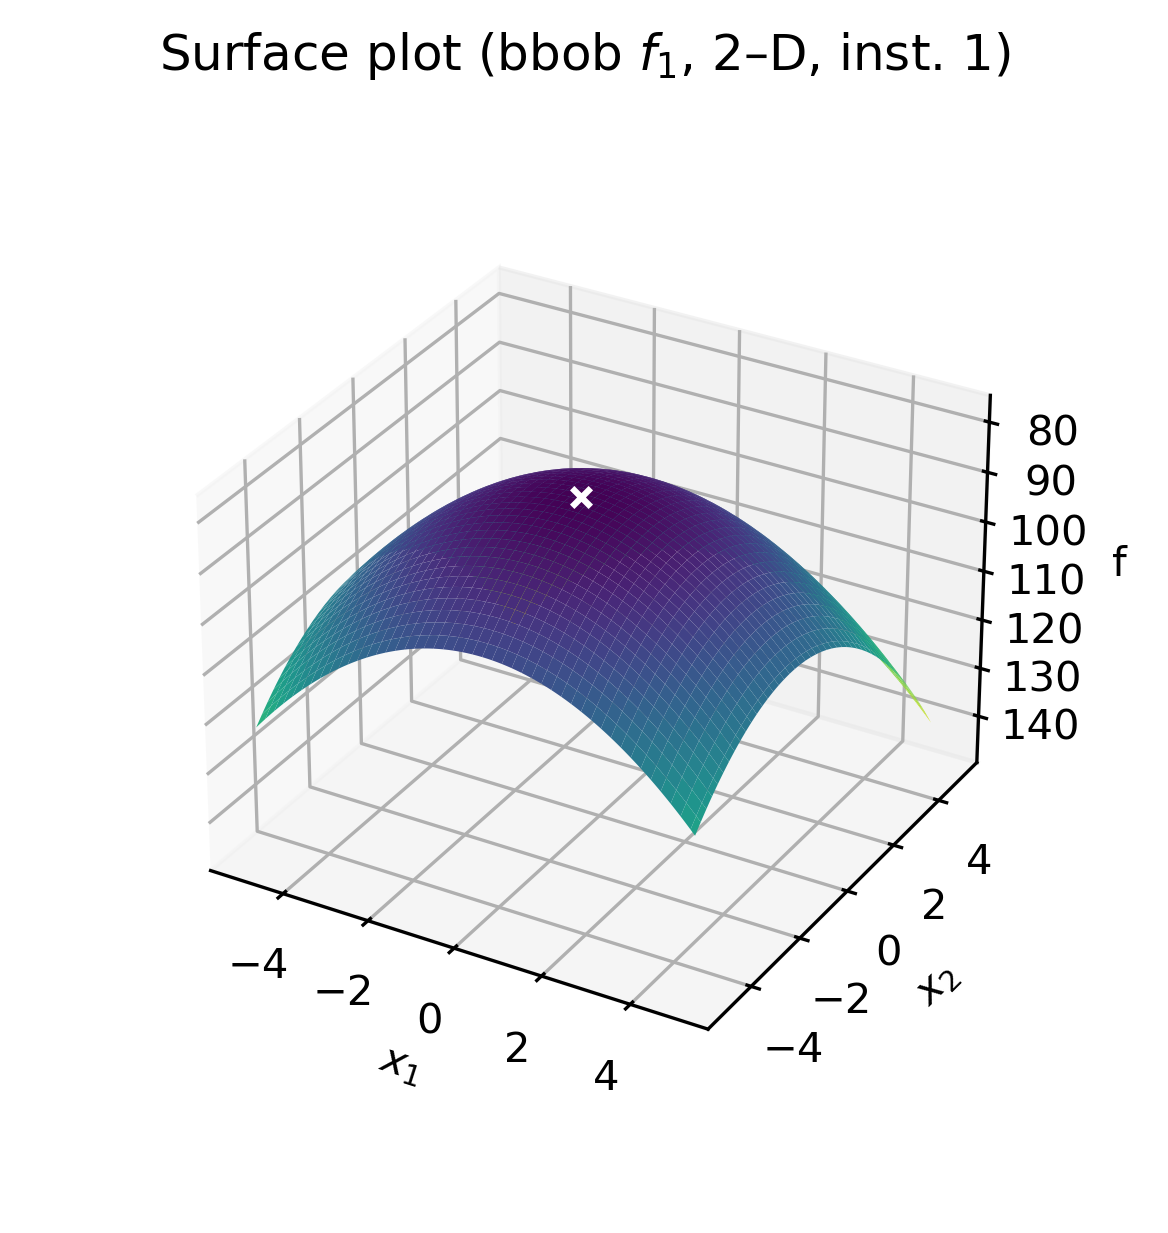
\includegraphics[width=\textwidth]{Slike/Diploma_slike/bbob_f001_i01_d02_surface.png}
        \caption{Ploskovni prikaz $f_1$}
        \label{fig:f1-surface}
    \end{subfigure}
    \hfill
    \begin{subfigure}[b]{0.38\textwidth}
        \centering
        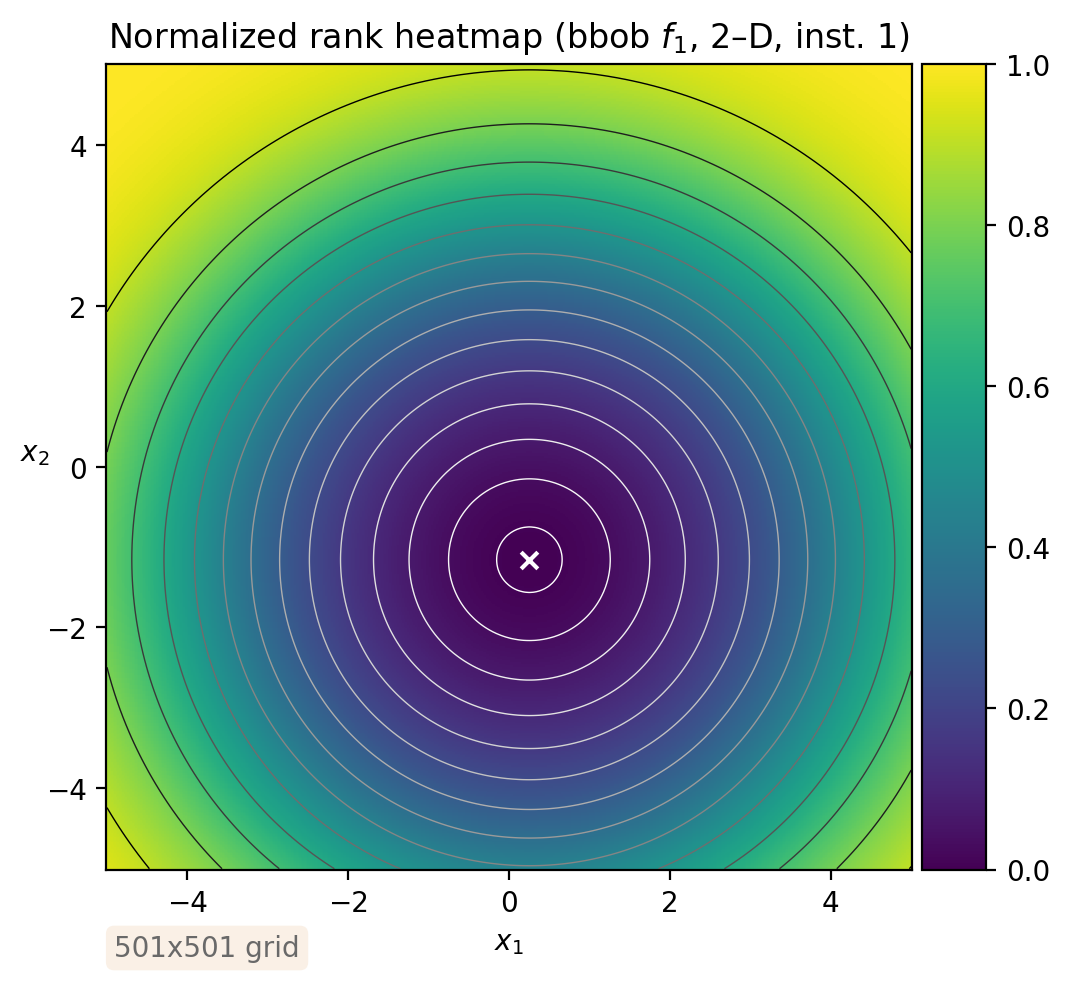
\includegraphics[width=\textwidth]{Slike/Diploma_slike/bbob_f001_i01_d02_heatmap-rank.png}
        \caption{Toplotna karta rangov $f_1$}
        \label{fig:f1-rank}
    \end{subfigure}

    \vspace{1em}

    \begin{subfigure}[b]{0.38\textwidth}
        \centering
        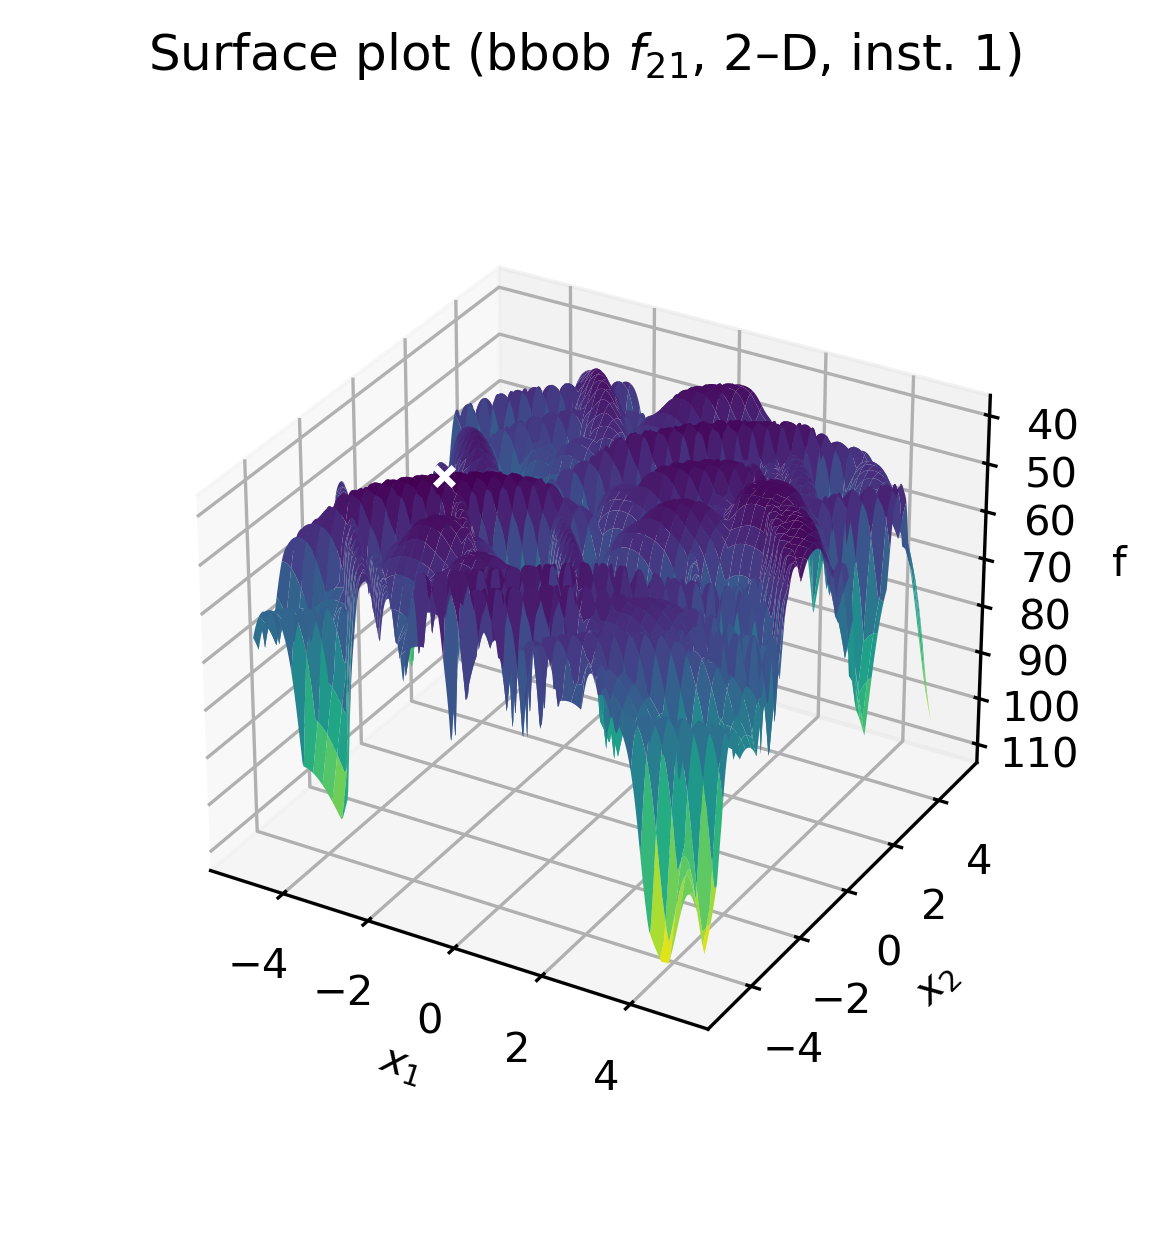
\includegraphics[width=\textwidth]{Slike/Diploma_slike/bbob_f021_i01_d02_surface.png}
        \caption{Ploskovni prikaz $f_{21}$}
        \label{fig:f21-surface}
    \end{subfigure}
    \hfill
    \begin{subfigure}[b]{0.38\textwidth}
        \centering
        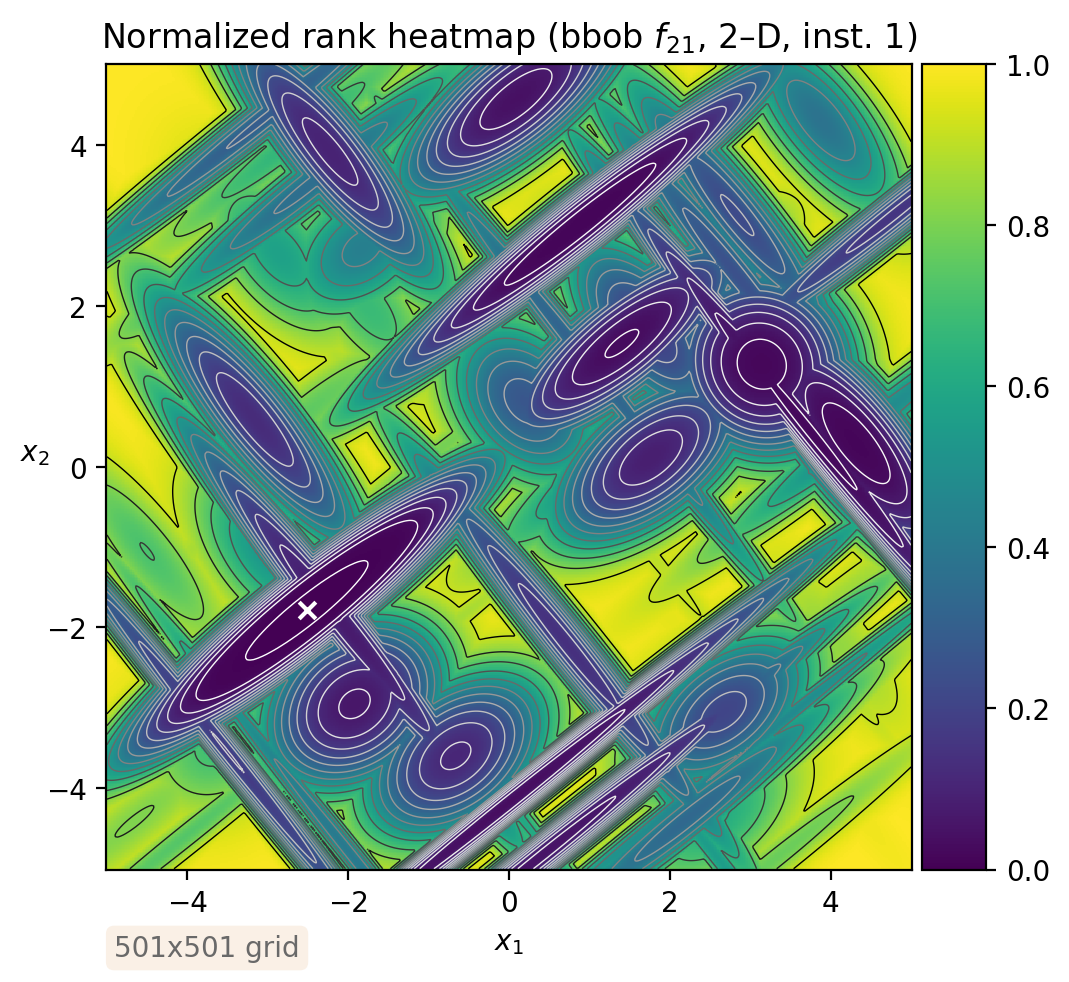
\includegraphics[width=\textwidth]{Slike/Diploma_slike/bbob_f021_i01_d02_heatmap-rank.png}
        \caption{Toplotna karta rangov $f_{21}$}
        \label{fig:f21-rank}
    \end{subfigure}

    \caption{Krajini funkcije sfere ($f_1$, zgoraj) in Gallagherjeve funkcije
    s 101 vrhom ($f_{21}$, spodaj) v dimenziji 2, prikazani kot ploskev (levo)
    in kot toplotna karta normaliziranih rangov (desno). Kontrast ponazarja
    razpon težavnosti nabora BBOB, od preproste unimodalne kotanje do močno
    multimodalne krajine s šibko globalno strukturo. Vir slik: okolje
    COCO~\cite{bbob2019}.}
    \label{fig:krajine}
\end{figure}



\chapter{Zajem in priprava podatkov}

Mere, ki jih predstavimo v naslednjem poglavju, ne delujejo neposredno na surovih podatkih iz zagona optimizacijskih algoritmov, temveč na podatkih, ki jih iz teh zagonov izpeljemo z dodatnim preoblikovanjem. V tem poglavju opišemo, kako te podatke zajamemo in pripravimo. Predstavimo orodji, s katerima izvedemo optimizacijske zagone, način zajema trajektorij populacije, ter postopek gručenja, s katerim trajektorije pretvorimo v obliko, primerno za analizo podobnosti.

\section{Pregled postopka}
\label{sec:pregled-postopka}

Preden se posvetimo posameznim korakom, si oglejmo postopek kot celoto.
Slika~\ref{fig:pipeline} prikazuje pot od izvajanja optimizacijskih
algoritmov do predstavitve, na kateri temeljijo mere podobnosti iz
poglavja~\ref{ch:metrike}. Vsakemu od korakov je posvečen eden od razdelkov
tega poglavja.

\begin{figure}[H]
\centering
\resizebox{\textwidth}{!}{%
\begin{tikzpicture}[
    node distance=6mm,
    box/.style={draw, rounded corners, align=center, font=\footnotesize,
                fill=blue!6, minimum height=11mm, text width=21mm,
                inner sep=2pt},
    boxwide/.style={box, text width=24mm},
    arr/.style={-{Latex[length=2mm]}}
]
\node[boxwide] (run) {Izvajanje algoritmov};
\node[box, right=of run] (traj) {Zajem trajektorij};
\node[box, right=of traj] (clu) {Gručenje (KMeans)};
\node[boxwide, right=of clu, fill=green!10] (dist) {Porazdelitev zasedenosti};
\node[box, right=of dist, fill=orange!10] (viz) {Vizualizacija};

\draw[arr] (run) -- (traj);
\draw[arr] (traj) -- (clu);
\draw[arr] (clu) -- (dist);
\draw[arr] (dist) -- (viz);

\node[below=6mm of dist, font=\footnotesize\itshape, text width=32mm, align=center]
    (metrike) {vhod v poglavje~\ref{ch:metrike}};
\draw[arr] (dist) -- (metrike);
\end{tikzpicture}%
}
\caption{Pregled postopka zajema in priprave podatkov: od izvajanja
algoritmov, prek zajema trajektorij, do gručenja in končne predstavitve v
obliki porazdelitve zasedenosti gruč. Zagone izvedemo s knjižnicama mealpy
in cocoex (razdelek~\ref{sec:mc}). Dobljena predstavitev je izhodišče tako
za ponazoritvene vizualizacije kot za mere podobnosti, obravnavane v
poglavju~\ref{ch:metrike}.}
\label{fig:pipeline}
\end{figure}


Programska koda celotnega cevovoda, od zagona algoritmov prek zajema
trajektorij in gručenja do izračuna mer podobnosti, je javno dostopna na
naslovu \url{https://github.com/8Timon24/Diploma-Analiza-in-vizualizacija-algoritmov-za-optimizacijo}.
Repozitorij vsebuje tudi datoteko \texttt{requirements.txt} z različicami
vseh uporabljenih knjižnic. Ker so naključna semena optimizacijskih
algoritmov fiksirana (razdelek~\ref{subsec:parametri}), so zagoni ponovljivi.

\section{Sorodna dela in izhodišče}
\label{sec:sorodna}

Motivacija za to delo je članek \emph{ClustOpt}~\cite{clustopt2025} skupaj s
spremljajočim konferenčnim prispevkom~\cite{cenikj2025searchbehavior}, v
katerih je opisan postopek za vizualizacijo in primerjavo optimizacijskih
algoritmov, ki temeljijo na metahevristikah. Postopek združuje odprtokodni knjižnici
\emph{mealpy} in \emph{cocoex} (predstavimo ju v razdelku~\ref{sec:mc}), ki
ponujata aktualen nabor metahevrističnih algoritmov in funkcij za njihovo
vrednotenje. Osrednja ideja pristopa je, da algoritmov ne primerjamo zgolj po
uspešnosti, temveč po njihovem \emph{vedenju} med iskanjem, ki ga zajamemo iz
trajektorij populacije.

Iz tega dela izhajata dva gradnika, na katerih gradimo tudi v tem delu:
postopek \emph{gručenja trajektorij} populacije, s katerim položaje agentov
skozi iteracije pretvorimo v obliko, primerno za analizo, ter \emph{kosinusna
mera podobnosti} med tako pridobljenimi predstavitvami. Ta dva gradnika
predstavljata izhodišče in ju v celoti prevzamemo. Podrobneje ju opišemo v
razdelkih~\ref{sec:grucenje} in~\ref{sec:cosine}.

Prispevek našega dela je razširitev tega izhodišča s \emph{petimi} dodatnimi
merami podobnosti, ki zajamejo različne vidike vedenja algoritmov. Te mere in
njihovo analizo podrobneje predstavimo v poglavju~\ref{ch:metrike},
razmejitev med prevzetim in izvirnim pa povzema
tabela~\ref{tab:pregled-mer}.

\section{Orodji mealpy in cocoex}
\label{sec:mc}

Za izvedbo optimizacijskih zagonov uporabimo dve odprtokodni knjižnici v
programskem jeziku Python: \emph{mealpy}, ki ponuja implementacije populacijskih
metahevrističnih algoritmov, in \emph{cocoex}, ki omogoča dostop do
primerjalnega nabora BBOB, predstavljenega v razdelku~\ref{sec:bbob}.

\subsection{mealpy}

Knjižnica \emph{mealpy}~\cite{van2023mealpy} (uporabljena različica 3.0.3)
vsebuje implementacije 233 metahevrističnih algoritmov, razvrščenih v
skupine glede na vir navdiha (evolucijski, rojni, fizikalni idr.), kot smo jih
opisali v razdelku~\ref{sec:opt_meta}. Iz tega nabora jih izberemo 28 iz različnih družin. Do te številke smo prišli s postopnim dodajanjem novih algoritmov, ko smo hoteli primerjati nekatere lastnosti in vedenje algoritmov. Večje število ne bi bilo smiselno, saj je večina vizualizacij narejena za primerjavo relativno majhnega števila algoritmov, tako da izmed teh 28 vzamemo še reprezentativno podmnožico, ki jo podrobneje analiziramo. 

Izbrani nabor pokriva šest od skupin, opisanih v razdelku~\ref{sec:opt_meta}:
šestnajst rojnih algoritmov, šest evolucijskih, tri sistemske ter po enega
predstavnika človeških, fizikalnih in matematičnih. Vseh 28 algoritmov skupaj
z njihovimi polnimi imeni in pripadajočo skupino navaja
tabela~\ref{tab:algoritmi}. V prvem stolpcu so imena zapisana tako, kot se
pojavljajo v knjižnici mealpy, saj v tej obliki nastopajo tudi v legendah
slik v poglavju~\ref{ch:rezultati}. Polna imena puščamo v angleščini, ker so
metode pod njimi uveljavljene v literaturi.

\begin{table}[H]
\centering
\small
\setlength{\tabcolsep}{5pt}
\begin{tabular}{@{}lll@{}}
\toprule
{\bf Algoritem} & {\bf Polno ime} & {\bf Skupina} \\
\midrule
\texttt{AugmentedAEO} & Augmented Artificial Ecosystem Optimization & sistemski \\
\texttt{GWO\_WOA} & Hybrid Grey Wolf and Whale Optimization Algorithm & rojni \\
\texttt{HI\_WOA} & Hybrid Improved Whale Optimization Algorithm & rojni \\
\texttt{IGWO} & Improved Grey Wolf Optimization & rojni \\
\texttt{ImprovedBSO} & Improved Brain Storm Optimization & človeški \\
\texttt{JADE} & Adaptive Differential Evolution with External Archive & evolucijski \\
\texttt{L\_SHADE} & SHADE with Linear Population Size Reduction & evolucijski \\
\texttt{LevyTWO} & Tug of War Optimization, Lévy flight variant & fizikalni \\
\texttt{ModifiedAEO} & Modified Artificial Ecosystem-based Optimization & sistemski \\
\texttt{OriginalAEO} & Artificial Ecosystem-based Optimization & sistemski \\
\texttt{OriginalALO} & Ant Lion Optimizer & rojni \\
\texttt{OriginalCSA} & Cuckoo Search Algorithm & rojni \\
\texttt{OriginalDE} & Differential Evolution & evolucijski \\
\texttt{OriginalFPA} & Flower Pollination Algorithm & evolucijski \\
\texttt{OriginalGWO} & Grey Wolf Optimizer & rojni \\
\texttt{OriginalHC} & Hill Climbing & matematični \\
\texttt{OriginalHHO} & Harris Hawks Optimization & rojni \\
\texttt{OriginalMFO} & Moth-Flame Optimization & rojni \\
\texttt{OriginalMPA} & Marine Predators Algorithm & rojni \\
\texttt{OriginalMRFO} & Manta Ray Foraging Optimization & rojni \\
\texttt{OriginalNMRA} & Naked Mole-Rat Algorithm & rojni \\
\texttt{OriginalSHADE} & Success-History Based Adaptive Differential Evolution & evolucijski \\
\texttt{OriginalSSA} & Sparrow Search Algorithm & rojni \\
\texttt{OriginalSSpiderA} & Social Spider Algorithm & rojni \\
\texttt{OriginalWOA} & Whale Optimization Algorithm & rojni \\
\texttt{RW\_GWO} & Random Walk Grey Wolf Optimizer & rojni \\
\texttt{SADE} & Self-Adaptive Differential Evolution & evolucijski \\
\texttt{WhaleFOA} & Whale Fruit-fly Optimization Algorithm & rojni \\
\bottomrule
\end{tabular}
\caption{28 metahevrističnih algoritmov, uporabljenih v tem delu, z njihovimi
polnimi imeni in skupino glede na vir navdiha. Skupine ustrezajo razdelitvi
knjižnice mealpy: rojni (\texttt{swarm\_based}), evolucijski
(\texttt{evolutionary\_based}), sistemski (\texttt{system\_based}), človeški
(\texttt{human\_based}), fizikalni (\texttt{physics\_based}) in matematični
(\texttt{math\_based}).}
\label{tab:algoritmi}
\end{table}

\subsection{cocoex}

Knjižnica \emph{cocoex}~\cite{hansen2021coco} (uporabljena različica 2.8.2) je
vmesnik do okolja COCO, prek katerega dostopamo do primerjalnega nabora BBOB.
Za dano funkcijo, instanco in dimenzijo cocoex vrne objekt problema, ki
podpira klic z vektorjem $x \in \mathbb{R}^n$ in vrne vrednost kriterijske funkcije $f(x) \in \mathbb{R}$, kar
ustreza obravnavi problema kot črne škatle.

\subsection{Parametri zagonov}
\label{subsec:parametri}

Vsak algoritem poženemo na vseh 24 funkcijah primerjalnega nabora BBOB, na
prvih petih instancah vsake funkcije ter v dimenzijah $n \in \{2, 5, 10\}$.
Vsako kombinacijo (algoritem, funkcija, instanca, dimenzija) ponovimo s petimi
semeni $s \in \{1,2,3,4,5\}$, ki so fiksna zaradi lažje ponovljivosti.
Velikost populacije je pri vseh zagonih $\mathit{pop\_size} = 50$, število iteracij pa
je odvisno od dimenzije, in sicer skladno s~\cite{clustopt2025} vzamemo $10n$,
kjer je $n$ dimenzija iskalnega prostora.

\section{Zajem trajektorij}
\label{sec:trajektorije}

Za vsako kombinacijo algoritma, funkcije, instance, dimenzije in naključnega
semena poženemo zagon optimizacijskega algoritma s pomočjo knjižnice mealpy in
med njegovim potekom zajamemo tri vrste podatkov: \emph{populacijsko
trajektorijo}, \emph{trajektorijo najboljše rešitve} in \emph{mero
raznolikosti populacije}.

\subsection{Populacijska trajektorija}

Za razliko od pristopov, ki beležijo le najboljšo najdeno rešitev, v tem delu
shranimo \emph{celotno populacijo} skozi vse iteracije zagona, saj mere
podobnosti temeljijo na tem, kako se populacija kot celota giblje po iskalnem
prostoru. Knjižnica mealpy med reševanjem v atributu
\texttt{model.history.list\_population} beleži pozicije vseh agentov v vsaki
iteraciji. Za vsakega agenta v vsaki iteraciji shranimo njegov položaj
$x \in \mathbb{R}^n$, vrednost kriterijske funkcije $f(x)$, zaporedno številko
iteracije ter kumulativno število dotedanjih vrednotenj kriterijske funkcije.

\subsection{Trajektorija najboljše rešitve}

Poleg celotne populacije shranimo tudi \emph{trajektorijo najboljše rešitve}
, torej zaporedje najboljših doslej najdenih rešitev skozi
iteracije, ki ga mealpy beleži v atributu
\texttt{model.history.list\_global\_best}. Ta trajektorija je za razliko od
populacijske trajektorije monotono nepadajoča v kakovosti rešitve in
predstavlja pot, po kateri se je premikala trenutno najboljša znana rešitev.

Ob koncu vsakega zagona shranimo tudi končno najboljšo rešitev in njeno
vrednost kriterijske funkcije v skupno datoteko rezultatov, ki jo v
poglavju~\ref{ch:metrike} uporabimo za izračun mer podobnosti končnih rešitev.

\subsection{Raznolikost populacije}

Za vsako iteracijo zagona mealpy izračuna tudi mero \emph{raznolikosti}
populacije, iz katere izpelje deleža \emph{raziskovanja} (angl.\ exploration)
in \emph{izkoriščanja} (angl.\ exploitation) v odstotkih, ki se v vsaki
iteraciji seštejeta v 100 \%. Raznolikost temelji na povprečnem odstopanju
položajev agentov od mediane populacije, delež raziskovanja pa je raznolikost,
normalizirana glede na največjo raznolikost, doseženo med celotnim zagonom.
Te vrednosti zajamemo iz atributov \texttt{model.history.list\_diversity},
\texttt{list\_exploration} in \texttt{list\_exploitation} ter jih uporabimo v
razdelku~\ref{sec:exploration} pri meri razlike v raziskovanju in
izkoriščanju.

Zajete podatke organiziramo v datotečno strukturo, ločeno po dimenziji,
algoritmu ter kombinaciji funkcije in instance, znotraj katere je vsak zagon
(identificiran z naključnim semenom) shranjen v svoji datoteki. Ločeno
shranimo tudi skupno datoteko končnih rezultatov na dimenzijo, ki vsebuje
najboljšo rešitev vsakega zagona.

\section{Gručenje trajektorij}
\label{sec:grucenje}

Populacijska trajektorija, kot jo zajamemo v razdelku~\ref{sec:trajektorije},
je zaporedje položajev velikega števila agentov skozi mnogo iteracij, kar samo
po sebi ni primerno za neposredno primerjavo med algoritmi. Zato trajektorije
najprej pretvorimo v jedrnatejšo predstavitev. Za vsak \emph{problem} (v tem in naslednjih poglavjih s tem izrazom vedno mislimo na eno samo,
fiksno kombinacijo funkcije \emph{in} instance, ne le funkcije) položaje
vseh agentov \emph{vseh algoritmov in vseh zagonov} združimo ter jih gručimo z
metodo KMeans. Rezultat je \emph{porazdelitev zasedenosti gruč}, ki je osnova za večino
mer podobnosti, predstavljenih v poglavju~\ref{ch:metrike}.

\subsection{Priprava podatkov}

Pred gručenjem podatke za posamezen problem filtriramo. Obdržimo le
algoritme iz obravnavanega nabora, odstranimo pa vrstice, ki ustrezajo
začetni (ničti) iteraciji, saj ta predstavlja naključno inicializacijo
populacije pred začetkom iskanja in ne dejanskega iskalnega vedenja.
Koordinate in vrednosti kriterijske funkcije nato skaliramo\footnote{Uporabimo min-max skaliranje}, da so med seboj primerljive ne glede na obseg
posamezne razsežnosti oziroma funkcije.

\subsection{Algoritem KMeans}

Cilj algoritma je razdeliti $N$ točk v $k$ gruč tako, da minimiziramo vsoto
kvadratov razdalj med vsako točko in centrom njene gruče (angl.\ within-cluster sum of squares,
\textbf{WCSS}):
\[
    \min_{\{C_1, \dots, C_k\}} \sum_{j=1}^{k} \sum_{x \in C_j} \lVert x - \mu_j \rVert^2,
\]
kjer je $C_j$ množica točk, dodeljenih $j$-ti gruči, $\mu_j$ pa njen center
(povprečje pripadajočih točk). Algoritem WCSS minimizira iterativno, z
izmeničnim ponavljanjem dveh korakov. Vsako točko dodeli najbližjemu
trenutnemu centru, nato vsak center posodobi kot povprečje njemu dodeljenih
točk. Postopek se ponavlja, dokler se dodelitve točk gručam ne prenehajo
spreminjati oziroma dokler se centri ne ustalijo.

Začetni položaj centrov pomembno vpliva na kakovost in hitrost konvergence,
zato uporabimo inicializacijo \emph{k-means++}, ki centre izbira zaporedno in
naključno, a s porazdelitvijo, sorazmerno kvadratu razdalje do najbližjega že
izbranega centra. S tem se začetni centri razpršijo po prostoru, kar
zmanjša tveganje slabe konvergence v primerjavi z zgolj naključno
inicializacijo.

KMeans je za naš namen primeren, ker zaradi uporabe evklidske razdalje in
posodabljanja centrov kot povprečij tvori gruče, ki so približno
\emph{sferične} oblike. Take gruče je lažje interpretirati kot posamezne
\sn{regije} iskalnega prostora primerljive velikosti v vseh smereh, kar je za našo analizo (kjer gručo beremo kot eno mesto, ki ga je populacija obiskala) bolj smiselno kot gruče poljubnih, podolgovatih ali
nekonveksnih oblik, ki bi jih lahko proizvedle druge metode gručenja.

\subsection{Izbira števila gruč}

Število gruč $k$ ni fiksno, temveč se za vsak problem posebej določi z
\emph{metodo komolca} (angl.\ elbow method). Ker se WCSS z večanjem $k$
vedno zmanjšuje (v skrajnem primeru $k=N$ je WCSS enaka 0), izbira zgolj
najmanjše WCSS ni smiselna. Namesto tega WCSS izrišemo kot funkcijo $k$ in
poiščemo točko, pri kateri se hitrost upadanja bistveno upočasni, t.\,i.\
\sn{komolec} krivulje. Do te točke dodajanje gruč še pomembno izboljša
prileganje, po njej pa prinaša le majhne dodatne izboljšave za ceno večje
kompleksnosti.

Komolec določimo samodejno za kandidatne vrednosti $k$, ki so potence
števila 2 od $k=4$ do $k=512$. Ta nabor kandidatov
pokrije širok razpon možnih velikosti brez potrebe po preizkušanju vsake
posamezne vrednosti $k$.

Za samodejno določitev komolca uporabimo razred \texttt{KElbowVisualizer} iz
knjižnice \emph{Yellowbrick}~\cite{bengfort2019yellowbrick}. Ta komolec
poišče z algoritmom zaznavanja kolena \emph{Kneedle}~\cite{satopaa2011kneedle},
ki za koleno vzame točko največje ukrivljenosti krivulje, torej tisto vrednost $k$, pri kateri se upadanje WCSS najizraziteje upočasni.

\subsection{Gručenje in porazdelitev zasedenosti}

Nad skaliranimi koordinatami agentov poženemo KMeans z izbranim številom
gruč. Uporabimo implementacijo iz knjižnice
\emph{scikit-learn}~\cite{pedregosa2011scikit}. Ker gručenje izvedemo \emph{skupno} za vse algoritme in zagone na
danem problemu, so oznake gruč med algoritmi neposredno primerljive. Ista
oznaka gruče pri dveh različnih algoritmih ustreza isti regiji iskalnega
prostora. Ta lastnost je ključna za smiselnost mer podobnosti, ki
porazdelitve zasedenosti med algoritmi neposredno primerjajo.
Za vsako kombinacijo algoritma, zagona in iteracije nato preštejemo koliko
agentov je pripadalo posamezni gruči, kar da tabelo porazdelitve zasedenosti gruč skozi čas, osrednjo predstavitev, na kateri temeljijo mere podobnosti
v poglavju~\ref{ch:metrike}.
Za vsak problem shranimo tri datoteke: koordinate centrov gruč, celoten
označen nabor podatkov (položaji agentov skupaj s pripadajočo oznako gruče)
ter tabelo porazdelitve zasedenosti gruč, ki je vhod za nadaljnjo analizo.
Eden izmed možnih načinov vizualizacije trajektorije potem izhaja direktno iz gručenja. V vsaki iteraciji se 50 agentov porazporedi v $k$ gruč (odvisno od problema), kar nam v kombinaciji z uporabo \emph{heatmapa}\footnote{Vizualizacija je iz knjižnice Seaborn} da spodnjo sliko ~\ref{fig:zasedenost-primer}.

\begin{figure}[H]
\centering
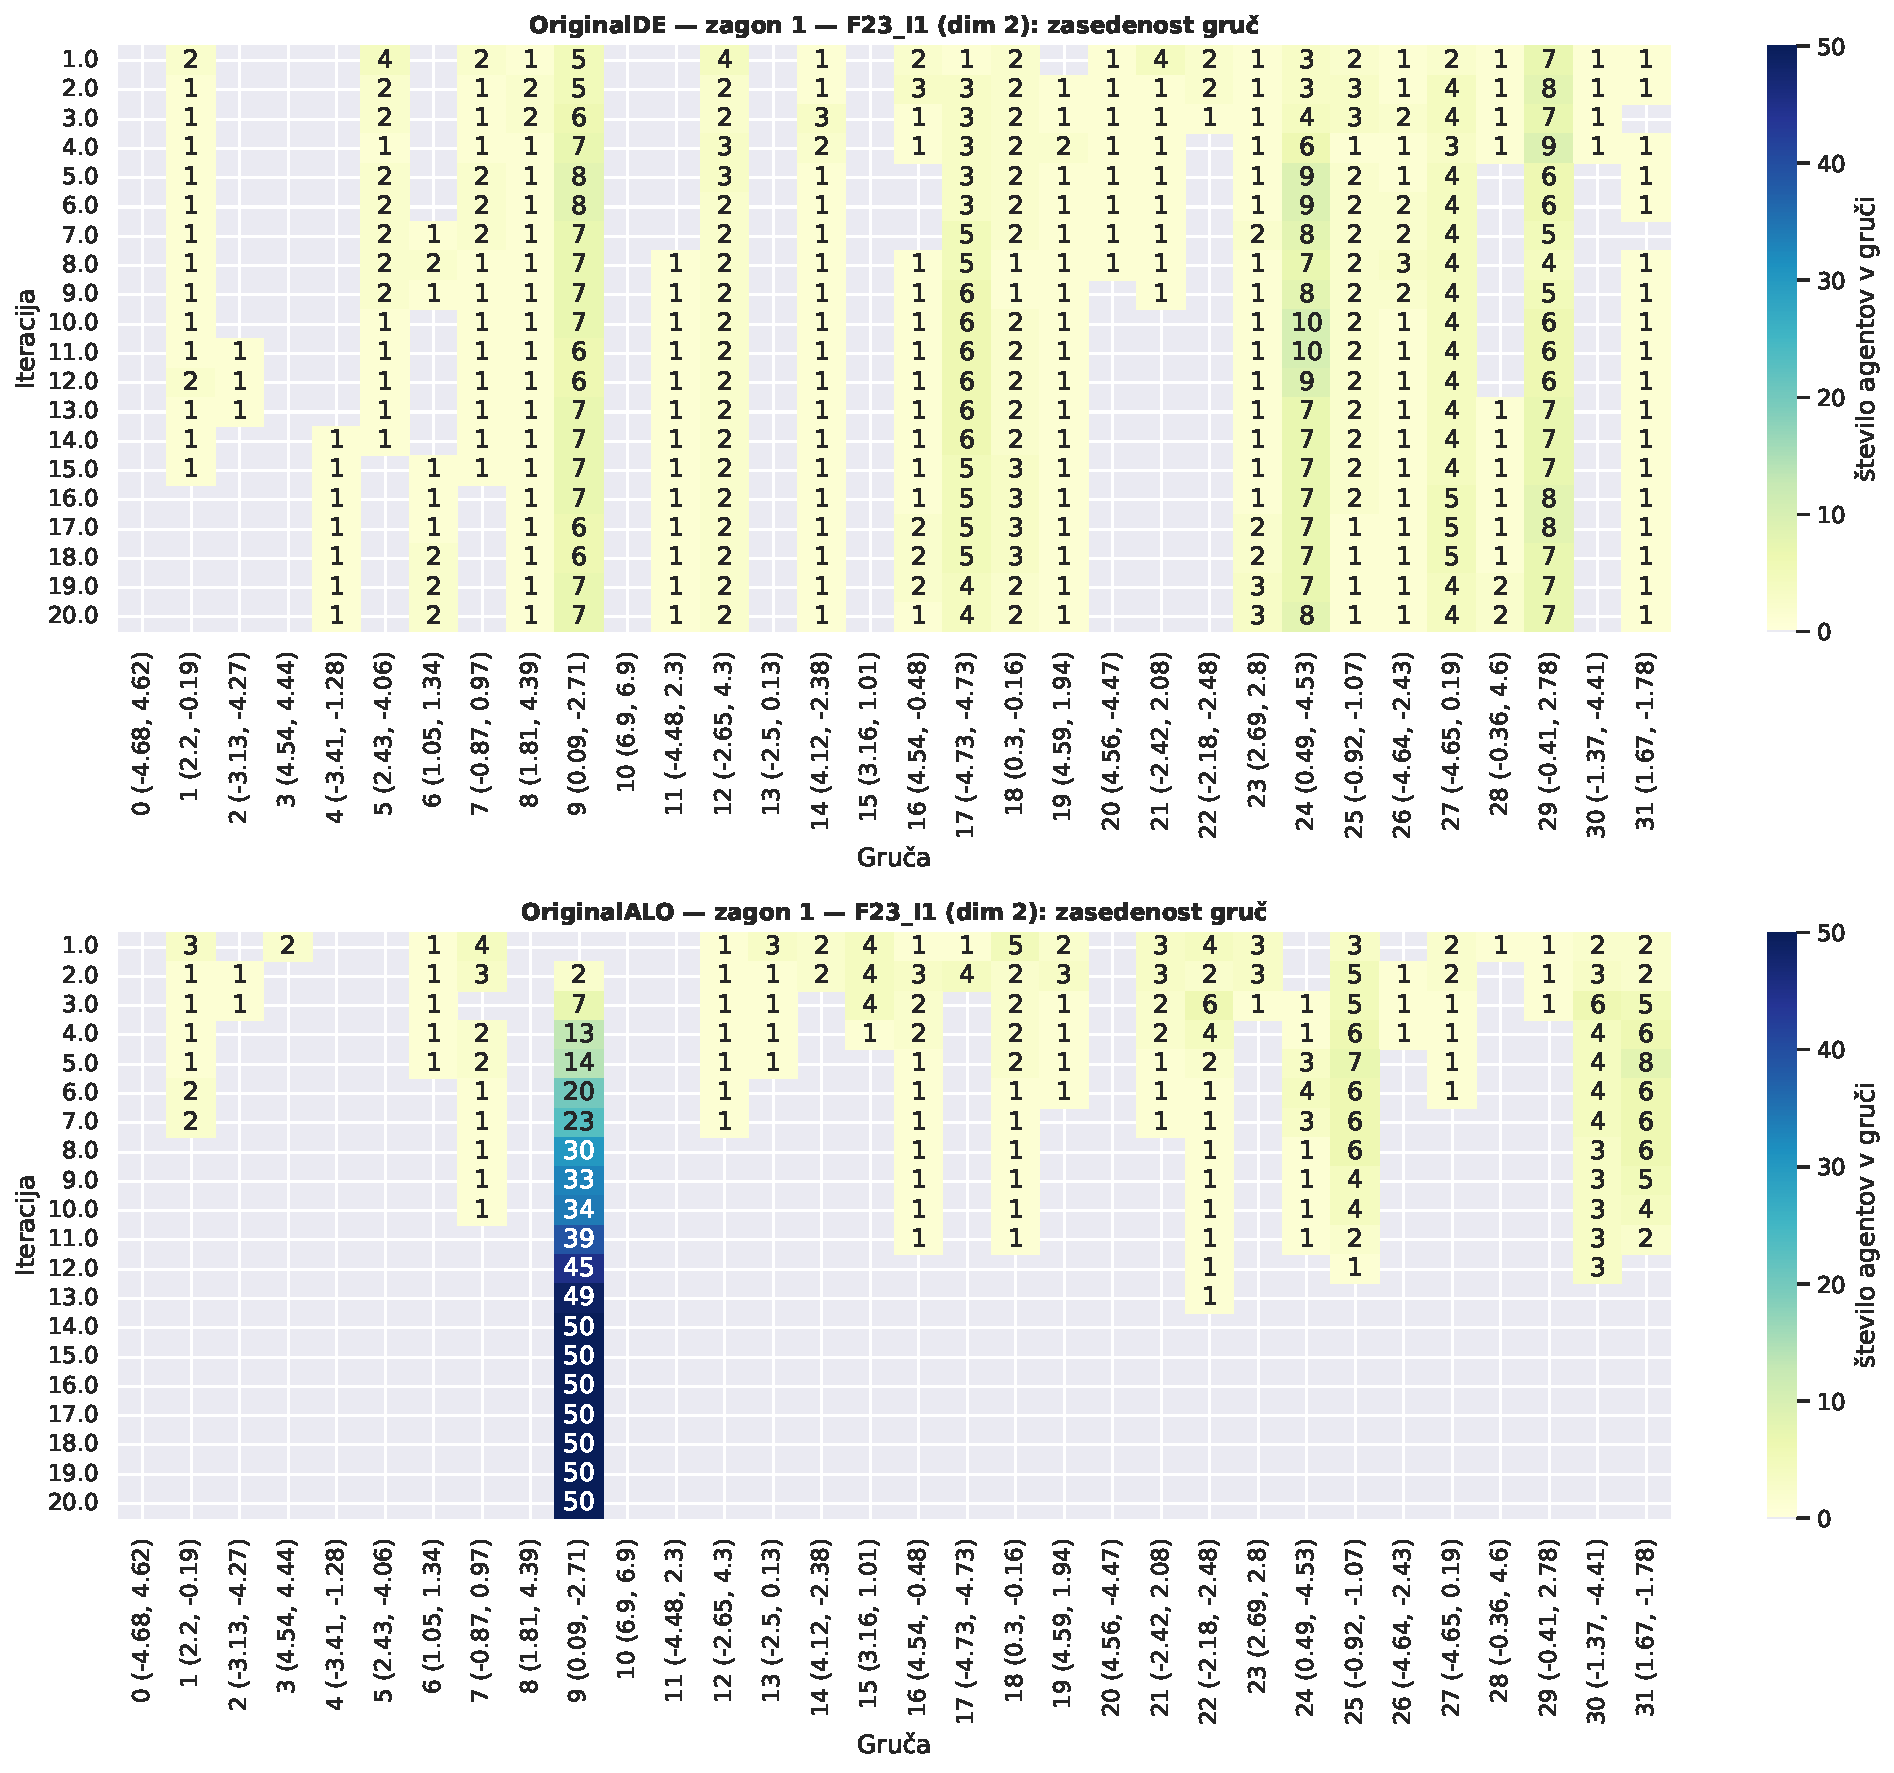
\includegraphics[width=0.85\textwidth]{Slike/Diploma_slike/clustering_latest_F23_I1_OriginalDE+OriginalALO_run_1_dim_2.pdf}
\caption{Porazdelitev zasedenosti gruč skozi iteracije za algoritma \emph{OriginalDE} in \emph{OriginalALO} na problemu $\prob{23}{1}$ (dimenzija 2, zagon 1).}
\label{fig:zasedenost-primer}
\end{figure}

Na sliki je razvidno, da na enem izmed težjih problemov algoritem \emph{OriginalDE} v 20 iteracijah
ni zmožen konvergirati, ne proti lokalnemu, ne proti globalnemu minimumu. Skozi vse iteracije je populacija zelo razkropljena in ni ene gruče v katero bi se algoritem bolj nagibal. 3 gruče so bolj \sn{obetavne}, ampak nobena ne prevlada. Na drugi strani se \emph{OriginalALO} začne nagibati h gruči 9 že zgodaj v zagonu, v 4. iteraciji že prevlada, čeprav še vedno poskuša malo raziskovati. V 14. iteraciji je pa že celotna njegova populacija v gruči z oznako 9. Pomembno je pa se zavedati, da to še ne pomeni da je \emph{OriginalALO} našel boljšo rešitev, ker je možno da se je ujel v lokalnem minimumu.


\chapter{Mere podobnosti}
\label{ch:metrike}

Vse mere podobnosti, predstavljene v tem poglavju, delijo skupno shemo. Za
poljuben par algoritmov na fiksni kombinaciji funkcije, instance in zagona
vsaka mera vrne eno samo številsko vrednost, ki je tem manjša, čim bolj
podobno sta se algoritma vedla. Mera entropije, obe kosinusni meri in mera
razlike v raziskovanju in izkoriščanju zavzemajo vrednosti na intervalu
$[0,1]$ (pri zadnji to dosežemo z delitvijo s 100, glej
razdelek~\ref{sec:exploration}), meri razlike v končni lokaciji in v končnem
fitnessu pa sta neomejeni.

Glede na Definicijo~\ref{def:metrika} velja pripomniti dvoje. Prvič, štiri od šestih mer (entropija, razlika v raziskovanju in izkoriščanju, razlika v
končni lokaciji in razlika v končnem fitnessu) so metrike na prostoru
\emph{predstavitev}, na katerih so definirane. Prvi dve sta, do
konstantnega faktorja $1/T$ natančno, razdalji $L^1$ med krivuljama v
$\mathbb{R}^T$, tretja je evklidska razdalja med točkama v $\mathbb{R}^n$,
četrta pa absolutna razlika realnih števil. Na prostoru \emph{algoritmov} pa
so le psevdometrike, saj preslikava iz algoritma v njegovo predstavitev ni
injektivna. Dva različna algoritma imata lahko na primer povsem enako
entropijsko krivuljo, čeprav sta pri tem zasedala različne gruče
(razdelek~\ref{sec:entropy}). Drugič, obe kosinusni meri kljub imenu
\sn{razdalja} nista niti psevdometriki, saj ne zadoščata trikotniški
neenakosti. Protiprimer navedemo v razdelku~\ref{sec:cosine}.

Glede izvora mer velja razmejitev. Globalna kosinusna razdalja
(razdelek~\ref{sec:cosine}) je v celoti prevzeta iz predhodnega
dela~\cite{clustopt2025}, predstavljenega v razdelku~\ref{sec:sorodna}, in
skupaj s postopkom gručenja iz razdelka~\ref{sec:grucenje} tvori izhodišče,
na katerem gradimo. Preostalih pet mer (entropija zasedenosti gruč,
kosinusna razdalja po gručah, razlika v raziskovanju in izkoriščanju, razlika
v končni lokaciji in razlika v končnem fitnessu) je prispevek tega dela.
Razmejitev skupaj z ostalimi lastnostmi mer povzema
tabela~\ref{tab:pregled-mer} na koncu poglavja.

Cilj tega poglavja ni izpostaviti eno samo, \sn{pravo} mero podobnosti,
temveč ponuditi nabor komplementarnih mer, od katerih vsaka zajame
drugačen vidik iskalnega vedenja algoritmov. Nekatere temeljijo na
porazdelitvi populacije po gručah, druge na razmerju med raziskovanjem in
izkoriščanjem, spet druge na doseženi kakovosti ali legi končne rešitve. Šele
skupaj te mere omogočajo celovitejši vpogled v podobnost dveh algoritmov, kot
bi ga dala katera koli izmed njih posamično.

\section{Entropija zasedenosti gruč}
\label{sec:entropy}

Ta mera meri, ali sta dva algoritma v posameznih trenutkih iskanja
populacijo agentov razporejala po iskalnem prostoru enako \emph{široko}. Če je
populacija razpršena po mnogih gručah, algoritem v tistem trenutku pretežno
raziskuje. Če je skoncentrirana v malo gručah, pretežno izkorišča.
Mera primerja, kako se ta širina spreminja skozi iteracije pri dveh
algoritmih, ne glede na to, katere gruče so pri tem zasedene.

\subsection{Formalna definicija}

Za dan algoritem in zagon na iteraciji $t$ naj $m_1, \dots, m_k$ označujejo
število agentov v vsaki od $k$ gruč tega problema, $M = \sum_{i=1}^k m_i$ pa
skupno število agentov.\footnote{Za zasedenosti gruč namenoma uporabljamo
simbol $m$ in ne $n$, ki je v tem delu rezerviran za dimenzijo iskalnega
prostora (razdelek~\ref{sec:opt_meta}).} Delež agentov v $i$-ti gruči je
$p_i = m_i / M$.
Shannonova entropija porazdelitve na iteraciji $t$ je
\[
    H(t) = -\sum_{i=1}^{k} p_i \ln p_i,
\]
pri čemer velja dogovor $0 \ln 0 = 0$.

Ker se število gruč $k$ med problemi razlikuje, bomo entropijo normalizirali
z njeno največjo možno vrednostjo. Ta je enaka $\ln k$, kar pokažemo v
Trditvi~\ref{trd:entropija-max}. Pri njenem dokazu potrebujemo Jensenovo
neenakost, ki jo zato navedemo najprej.

\begin{lema}[Jensenova neenakost, končna oblika]
\label{lema:Jensen}
Naj bo $f$ konkavna funkcija na intervalu $I \subseteq \mathbb{R}$, naj bodo
$x_1, \dots, x_n \in I$ in naj bodo $\lambda_1, \dots, \lambda_n \ge 0$ taki,
da je $\sum_{i=1}^n \lambda_i = 1$. Tedaj velja
\[
    \sum_{i=1}^{n} \lambda_i f(x_i) \le f\!\left( \sum_{i=1}^{n} \lambda_i x_i \right).
\]
Če je $f$ strogo konkavna, velja enakost natanko tedaj, ko so vsi $x_i$, za
katere je $\lambda_i > 0$, med seboj enaki~\cite[Izrek 2.6.4]{cover2006elements}.
\end{lema}

\begin{dokaz}
Navedemo le idejo. Za $n=2$ je trditev natanko definicija konkavnosti
funkcije $f$, splošni primer pa sledi z indukcijo na $n$.
\end{dokaz}


\begin{trditev}
\label{trd:entropija-max}
Naj bo $p = (p_1, \dots, p_k)$ diskretna porazdelitev na $k$ izidih 
(torej $p_i \ge 0$ in $\sum_{i=1}^k p_i = 1$), in naj bo
$H(p) = -\sum_{i=1}^k p_i \ln p_i$. Tedaj velja
\[
    H(p) \le \ln k,
\]
z enakostjo natanko tedaj, ko je $p_i = 1/k$ za vsak $i$.
\end{trditev}

\begin{dokaz}
Funkcija $f(x) = -x \ln x$ je na $(0, \infty)$ strogo konkavna, saj je
$f''(x) = -1/x < 0$. Z dogovorom $f(0) = 0$ je zvezna in strogo konkavna na
celotnem $[0, \infty)$, zato spodnji sklep velja tudi tedaj, ko je kateri od
$p_i$ enak 0. Po Jensenovi neenakosti (Lema~\ref{lema:Jensen}) za konkavne funkcije, uporabljeni
z enakimi utežmi $1/k$, velja
\[
    \frac{1}{k} \sum_{i=1}^{k} f(p_i) \le f\!\left( \frac{1}{k} \sum_{i=1}^{k} p_i \right)
    = f\!\left(\frac{1}{k}\right),
\]
kjer smo upoštevali $\sum_i p_i = 1$. Množenje s $k$ da
\[
    \sum_{i=1}^{k} f(p_i) \le k \cdot f\!\left(\frac{1}{k}\right)
    = k \cdot \left(- \frac{1}{k} \ln \frac{1}{k}\right) = \ln k,
\]
kar je natanko $H(p) \le \ln k$. Ker je $f$ strogo konkavna, v Jensenovi
neenakosti velja enakost natanko tedaj, ko so vsi argumenti $p_1, \dots, p_k$
med seboj enaki. Skupaj s pogojem $\sum_i p_i = 1$ to pomeni $p_i = 1/k$ za
vsak $i$.
\end{dokaz}

Ker se število gruč $k$ med problemi
in dimenzijami razlikuje, entropijo normaliziramo z njeno največjo možno
vrednostjo $\ln k$ (Trditev~\ref{trd:entropija-max}):
\[
    \hat{H}(t) = \frac{H(t)}{\ln k} \in [0, 1].
\]
Pri tem privzamemo $k \ge 2$. Pri $k = 1$ je $\ln k = 0$ in izraz ni
definiran, a gre za izrojen primer, saj so tedaj vsi agenti nujno v isti
gruči, torej je $H(t) = 0$ za vsak $t$ in po dogovoru postavimo
$\hat{H}(t) = 0$. V praksi do tega ne pride, ker je najmanjše kandidatno
število gruč $k = 4$ (razdelek~\ref{sec:grucenje}).
Normalizacija je nujna za primerljivost mere med problemi in dimenzijami, saj
imajo ti lahko različno število gruč $k$. Za par algoritmov $A$ in $B$ na istem 
zagonu je mera \emph{razlike v entropiji} povprečje absolutnih razlik normaliziranih 
entropij po vseh $T$ iteracijah zagona:
\[
    d_H(A, B) = \frac{1}{T} \sum_{t=1}^{T} \left| \hat{H}_A(t) - \hat{H}_B(t) \right|.
\]

\subsection{Pomen mere entropije}

Mera $d_H$ zavzema vrednosti v $[0, 1]$, saj sta $\hat{H}_A(t)$ in
$\hat{H}_B(t)$ za vsak $t$ v $[0,1]$. Vrednost 0 pomeni, da sta algoritma na
vsaki iteraciji ohranjala enako diverziteto populacije po gručah, vrednost bliže
1 pa, da se je njuna širina raziskovanja skozi čas bistveno razlikovala.
Kar mera ne zajame, pa je, kje v iskalnem prostoru je algoritem razporejal
agente. Dva algoritma imata lahko popolnoma enako entropijsko krivuljo, 
medtem ko sta v resnici zasedala povsem različne gruče. 
To razliko naslavljajo mere, predstavljene v naslednjih razdelkih.

\section{Kosinusna razdalja (globalna)}
\label{sec:cosine}

Ta mera meri, ali sta dva algoritma skozi celoten zagon populacijo
razporejala po gručah na podoben način, pri čemer upošteva celotno
tabelo zasedenosti gruč naenkrat, ne le njeno širino v posamezni
iteraciji (kot entropija), temveč tudi, \emph{katere} gruče so bile
zasedene in kdaj. Mero smo prevzeli iz predhodnega dela~\cite{clustopt2025},
predstavljenega v razdelku~\ref{sec:sorodna}.

\subsection{Formalna definicija}

Za dan algoritem in zagon naj $m_{t,i}$ označuje število agentov v $i$-ti
gruči na iteraciji $t$, za $t = 1, \dots, T$ in $i = 1, \dots, k$. Tabelo
zasedenosti sploščimo v en sam vektor
\[
    v = (m_{1,1}, \dots, m_{1,k},\ m_{2,1}, \dots, m_{2,k},\ \dots,\
         m_{T,1}, \dots, m_{T,k}) \in \mathbb{R}^{Tk},
\]
tako da si iteracije sledijo po vrsti. Za par
algoritmov $A$ in $B$ na istem zagonu (torej z enako dolgim $T$ in enakim
številom gruč $k$, saj gručenje poteka skupno za ves problem) dobimo vektorja
$v_A, v_B \in \mathbb{R}^{Tk}$, v katerih so iteracije in gruče \emph{poravnane}. 
Kosinusna razdalja med njima je:
\[
    d_{\cos}(A, B) = 1 - \frac{v_A \cdot v_B}{\lVert v_A \rVert \, \lVert v_B \rVert}.
\]

\subsection{Pomen mere}

Ker vektorja $v_A, v_B$ vsebujeta le nenegativne vrednosti (števila
agentov), je njun kosinus vedno v $[0,1]$, zato je $d_{\cos} \in [0,1]$.
Vrednost 0 pomeni, da sta algoritma zasedala gruče v enakem sorazmerju ob
enakih iteracijah. Vrednost bliže 1 pomeni, da nista nikoli hkrati
zasedala istih gruč ob istih iteracijah.

Mera upošteva celoten vzorec zasedenosti, ne le njegovo širino ali samo množico obiskanih gruč.
Ima pa dve pomembni omejitvi. Prvič, ker primerja $t$-to iteracijo
algoritma $A$ neposredno s $t$-to iteracijo algoritma $B$, je \emph{časovno
toga}. Če bi algoritem $B$ sledil povsem enakemu vzorcu kot $A$, a z
zamikom nekaj iteracij, bi mera to zaznala kot veliko razliko, čeprav bi
šlo za skoraj enako vedenje. Drugič, kosinusna podobnost je
neobčutljiva na \emph{magnitudo}. Vektorja, ki kažeta v isto smer, a se
razlikujeta po velikosti komponent (npr. ena gruča z enim agentom v
primerjavi z gručo, ki jih ima štirideset), dasta enako kosinusno
podobnost.

Poleg tega $d_{\cos}$ kljub imenu \sn{razdalja} ni metrika v smislu
Definicije~\ref{def:metrika}, saj ne zadošča trikotniški neenakosti. Za
vektorje $u = (1,0)$, $v = (1,1)$ in $w = (0,1)$ namreč velja
\[
    d_{\cos}(u,v) = d_{\cos}(v,w) = 1 - \tfrac{1}{\sqrt{2}} \approx 0{,}293,
    \qquad
    d_{\cos}(u,w) = 1,
\]
torej $d_{\cos}(u,w) = 1 > 0{,}586 \approx d_{\cos}(u,v) + d_{\cos}(v,w)$.
Izraz \sn{razdalja} zato uporabljamo v ohlapnem pomenu mere različnosti in ne
v strogem metričnem pomenu. Isto velja za mero iz
razdelka~\ref{sec:cosine-columns}, ki je prav tako grajena na kosinusni
podobnosti.

\section{Stabilnost in podobnost algoritmov}
\label{sec:stabilnost-def}

Kosinusno podobnost iz razdelka~\ref{sec:cosine} lahko uporabimo tudi
drugače kot za primerjavo dveh algoritmov na istem zagonu. V tem razdelku
uvedemo dve taki uporabi: stabilnost posameznega algoritma glede na
inicializacijo in agregirano podobnost med parom algoritmov. Oba pojma sta,
skupaj s kosinusno podobnostjo, na kateri temeljita, v celoti prevzeta iz
predhodnega dela~\cite{clustopt2025} (razdelek~\ref{sec:sorodna}). Novo je le
to, da ju uporabimo na širšem naboru algoritmov in dimenzij. Rezultate
predstavimo v razdelku~\ref{sec:stabilnost}.

\subsection{Stabilnost}

Kosinusno podobnost lahko uporabimo kot oceno, kako občutljiv je algoritem
glede na različne inicializacije na istem problemu. Gledamo torej, kako se
njegova populacija skozi iteracije drugače premika v različnih zagonih
fiksnega problema. Temu pojmu občutljivosti na inicializacijo rečemo
\emph{stabilnost}.

\begin{definicija}
\label{def:stabilnost}
    Naj bo $R$ množica naključnih semen, uporabljenih pri različnih izvedbah
algoritma $a$ na problemu $p$, in naj $v_{a,p,r} \in \mathbb{R}^{Tk}$
označuje vektorsko predstavitev trajektorije (sploščeno tabelo zasedenosti
gruč, glej razdelek~\ref{sec:cosine}) algoritma $a$ na problemu $p$ pri
semenu $r$. Stabilnost algoritma $a$ na problemu $p$ definiramo kot
povprečno kosinusno podobnost med trajektorijami, pridobljenimi z različnimi
semeni~\cite{clustopt2025}:
\[
    \mathrm{stability}(a, p) = \frac{1}{|R|(|R|-1)}
    \sum_{\substack{r_k, r_l \in R \\ r_k \neq r_l}}
    \mathrm{sim}\bigl(v_{a,p,r_k},\, v_{a,p,r_l}\bigr),
\]
kjer je $\mathrm{sim}(\cdot,\cdot)$ kosinusna podobnost, definirana v
razdelku~\ref{sec:cosine}.
\end{definicija}

V nasprotju s preostalimi merami v tem poglavju je $\mathrm{stability}$
\emph{podobnost}, ne razdalja. Vrednost blizu 1 pomeni, da je algoritem
stabilen (neobčutljiv na inicializacijo), vrednost blizu 0 pa, da je njegovo
vedenje močno odvisno od naključnega semena.

\subsection{Podobnost med algoritmi}

Če pa hočemo paroma primerjati algoritme, lahko spet uporabimo kosinusno
podobnost, le da tokrat algoritma primerjamo na istih semenih, da izločimo
morebitni moteči dejavnik različne inicializacije.

\begin{definicija}
\label{def:similarity}
    Naj bo $P$ množica vseh obravnavanih problemov, preostala notacija pa enaka
kot zgoraj~\cite{clustopt2025}:
    \[
    \mathrm{similarity}(a_m, a_n) = \frac{1}{|R||P|}
    \sum_{r \in R} \sum_{p \in P}
    \mathrm{sim}\bigl(v_{a_m,p,r},\, v_{a_n,p,r}\bigr),
    \]
\end{definicija}

Zgornji izraz je agregacija kosinusne razdalje $d_{\cos}$ iz
razdelka~\ref{sec:cosine} čez vsa semena in vse probleme. Ta izračun
uporabimo za vizualizacijo gručenja algoritmov glede na kosinusno razdaljo,
ki jo predstavimo v razdelku~\ref{sec:grucenje-metrike}.

\section{Kosinusna razdalja po gručah}
\label{sec:cosine-columns}

Ta mera je naša različica globalne kosinusne razdalje iz
razdelka~\ref{sec:cosine}, ki namesto cele tabele zasedenosti naenkrat
primerja \emph{vsako gručo posebej}, njeno časovno vrsto zasedenosti skozi zagon, rezultate pa
nato povpreči po gručah. S tem zajame, ali sta algoritma posamezno regijo
iskalnega prostora zasedala z enakim \emph{časovnim ritmom}, kar je
informacija, ki jo globalna različica pri sploščitvi izgubi.

\subsection{Formalna definicija}

Za dan algoritem in zagon naj $a_i = (m_{1,i}, \dots, m_{T,i}) \in
\mathbb{R}^T$ označuje časovno vrsto zasedenosti $i$-te gruče skozi $T$ iteracij, torej zaporedje vrednosti, ki podaja, koliko agentov je gruča 
$i$ vsebovala na vsaki posamezni iteraciji zagona. Za par algoritmov $A$ in $B$ 
na istem zagonu naj bosta $a_i$ in $b_i$ pripadajoči časovni vrsti $i$-te gruče. 
Za vsako gručo $i = 1,\dots, k$ definiramo prispevek $s_i$ po pravilu:
\[
    s_i =
    \begin{cases}
        \text{(gruča $i$ se izloči iz povprečja)} & \text{če } a_i = \mathbf{0} \text{ in } b_i = \mathbf{0}, \\[4pt]
        0 & \text{če natanko eden od } a_i, b_i \text{ je } \mathbf{0}, \\[4pt]
        \dfrac{a_i \cdot b_i}{\lVert a_i \rVert \, \lVert b_i \rVert} & \text{sicer.}
    \end{cases}
\]
Prvi primer ustreza gruči, ki je noben algoritem nikoli ni obiskal, in je
zato za primerjavo irelevantna. Drugi primer ustreza gruči, ki jo je obiskal
natanko eden od algoritmov. Kosinus tu ni definiran (ker je eden od
vektorjev ničeln), zato prispevek po dogovoru postavimo na 0, kar ohrani
signal, da je en algoritem raziskoval nekam, kamor drugi ni šel. Naj bo
$K$ množica gruč, ki niso izločene po prvem pravilu. Mera \emph{kosinusne
razdalje po gručah} je
\[
    d_{\text{col}}(A, B) = 1 - \frac{1}{|K|} \sum_{i \in K} s_i.
\]

\subsection{Pomen mere}

Ker je vsak $s_i \in [0,1]$, velja tudi $d_{\text{col}} \in [0,1]$. Vrednost
0 pomeni, da sta algoritma vsako skupno obiskano gručo zasedala z enakim
časovnim ritmom, vrednost bliže 1 pa vse večje neujemanje.

Mera naslavlja časovno togost globalne kosinusne razdalje, saj primerjavo
loči po posameznih regijah. Deli pa njeno omejitev glede magnitude.
Gruča, kjer je en algoritem poslal enega samega agenta, drugi pa nobenega,
prispeva enako (ničelno) vrednost kot gruča, kjer bi en algoritem poslal
petdeset agentov, drugi pa nobenega, čeprav gre za vsebinsko precej
različni situaciji. 

\section{Razlika v raziskovanju in izkoriščanju}
\label{sec:exploration}

Ta mera meri, ali sta dva algoritma skozi zagon ohranjala podobno razmerje
med \emph{raziskovanjem} (angl.\ exploration) in \emph{izkoriščanjem} (angl.\
exploitation) iskalnega prostora. Za razliko od preostalih mer, ki temeljijo 
na gručah, ta izhaja iz knjižnice \emph{mealpy}. Ta neodvisnost je pomembna. Morebitno ujemanje te mere z na gručah temelječimi merami (na
primer z entropijo iz razdelka~\ref{sec:entropy}) bi kazalo na to, da dva
neodvisna vira merjenja prihajata do skladnih zaključkov o razpršenosti
populacije.

\subsection{Formalna definicija}
 
Za dan algoritem in zagon nam knjižnica mealpy za vsako iteracijo $t$ poda
delež \emph{raziskovanja} $e(t) \in [0, 100]$, ki odraža razpršenost
populacije v tisti iteraciji glede na razpršenost, doseženo  kadarkoli med
zagonom. To vrednost mealpy izračuna interno. Delež
\emph{izkoriščanja} je $100 - e(t)$. Ker se deleža na vsaki
iteraciji seštejeta v 100, en sam par vrednosti ($e(t)$ za oba algoritma) v
celoti opiše razmerje med raziskovanjem in izkoriščanjem. Ločene mere za
izkoriščanje zato ne potrebujemo.
 
Za par algoritmov $A$ in $B$ na istem zagonu je mera \emph{razlike v
raziskovanju in izkoriščanju} povprečje absolutnih razlik deležev
raziskovanja po vseh $T$ iteracijah zagona:
\[
    d_e(A, B) = \frac{1}{100\,T} \sum_{t=1}^{T} \left| e_A(t) - e_B(t) \right|.
\]
Faktor $1/100$ je zgolj pretvorba iz odstotkov v delež. Brez njega bi mera
zavzemala vrednosti na $[0,100]$, s tem pa je, tako kot preostale na gručah
temelječe mere, omejena na $[0,1]$.
 
\subsection{Pomen mere}
 
Mera $d_e$ zavzema vrednosti v $[0, 1]$. Vrednost
0 pomeni, da sta algoritma na vsaki iteraciji ohranjala enako razmerje med
raziskovanjem in izkoriščanjem, večja vrednost pa pomeni, da se je to
razmerje med njima skozi zagon bolj razlikovalo. 
Ker mera izvira iz povsem drugega vira podatkov kot na gručah temelječe
mere, ne pove ničesar o tem, \emph{katere} regije iskalnega prostora je
algoritem zasedal temveč meri izključno dinamiko prehajanja med raziskovanjem
in izkoriščanjem, ne glede na to, kje v prostoru se je to dogajalo. 

\section{Razlika v končni lokaciji}
\label{sec:location}

Ta mera meri, kako blizu druga drugi sta v iskalnem prostoru pristali
končni najboljši rešitvi dveh algoritmov.

\subsection{Formalna definicija}

Naj bosta $x^{*}_A, x^{*}_B \in \mathbb{R}^n$ končni najboljši rešitvi
(položaja $g\_best$) algoritmov $A$ in $B$ na istem zagonu. Mera razlike v
končni lokaciji je evklidska razdalja med njima:
\[
    d_{\text{loc}}(A, B) = \lVert x^{*}_A - x^{*}_B \rVert_2
    = \sqrt{\sum_{j=1}^{n} \left( x^{*}_{A,j} - x^{*}_{B,j} \right)^2}.
\]

\subsection{Pomen mere}

Mera je smiselna le znotraj iste instance problema, saj je lega optimuma
odvisna od instance (razdelek~\ref{sec:bbob}). Primerjava lokacij med
različnimi instancami ne bi bila smiselna, ker gre za različno premaknjene in zarotirane funkcije. Prav tako magnituda mere ni neposredno
primerljiva med dimenzijami, saj z večanjem $n$ narašča tudi razpon možnih
evklidskih razdalj znotraj iskalnega prostora $[-5,5]^n$.

\section{Razlika v končnem fitnessu}
\label{sec:fitness}

Ta mera meri razliko v doseženi kakovosti rešitve dveh algoritmov, torej
razliko v vrednosti kriterijske funkcije njunih končnih najboljših rešitev.

\subsection{Formalna definicija}

Naj bosta $y^{*}_A = f(x^{*}_A)$ in $y^{*}_B = f(x^{*}_B)$ končni vrednosti
kriterijske funkcije, ki ju dosežeta algoritma $A$ in $B$ na istem zagonu.
Mera razlike v končnem fitnessu je
\[
    d_{\text{fit}}(A, B) = \left| y^{*}_A - y^{*}_B \right|.
\]

\subsection{Pomen mere}

Ker primerjani vrednosti izhajata neposredno iz surove kriterijske funkcije,
mera pove, kako različno dobri sta bili končni rešitvi dveh algoritmov
\emph{med seboj}, ne pa, kako blizu je katera od njiju resničnemu
globalnemu optimumu. Ker je razpon vrednosti kriterijske funkcije med
različnimi funkcijami nabora BBOB izjemno velik, je mera smiselno
primerljiva le znotraj istega problema, ne pa med različnimi problemi.

\section{Pregled mer}
\label{sec:pregled-mer}

Tabela~\ref{tab:pregled-mer} strne šest mer, obravnavanih v tem poglavju:
njihove oznake, vir podatkov, iz katerega izhajajo, zalogo vrednosti, status
glede na Definicijo~\ref{def:metrika} ter razmejitev med prevzetim in
izvirnim. Stabilnosti in podobnosti iz razdelka~\ref{sec:stabilnost-def} v
tabelo ne vključujemo, saj gre za podobnosti in ne za razdalje.

\begin{table}[H]
\centering
\small
\setlength{\tabcolsep}{4pt}
\begin{tabular}{@{}llllcl@{}}
\toprule
{\bf Mera} & {\bf Oznaka} & {\bf Vir podatkov} & {\bf Zaloga} & {\bf Metrika} & {\bf Izvor} \\
\midrule
Entropija zasedenosti gruč    & $d_H$              & gručenje       & $[0,1]$      & da$^{*}$ & izvirna \\
Kosinusna razdalja            & $d_{\cos}$         & gručenje       & $[0,1]$      & ne       & prevzeta~\cite{clustopt2025} \\
Kosinusna razdalja po gručah  & $d_{\mathrm{col}}$ & gručenje       & $[0,1]$      & ne       & izvirna \\
Razlika v raziskovanju        & $d_e$              & mealpy         & $[0,1]$      & da$^{*}$ & izvirna \\
Razlika v končni lokaciji     & $d_{\mathrm{loc}}$ & končne rešitve & $[0,\infty)$ & da$^{*}$ & izvirna \\
Razlika v končnem fitnessu    & $d_{\mathrm{fit}}$ & končne rešitve & $[0,\infty)$ & da$^{*}$ & izvirna \\
\bottomrule
\end{tabular}
\caption{Pregled šestih mer podobnosti, obravnavanih v tem poglavju.
$^{*}$Metrika na prostoru predstavitev, na katerem je mera definirana. Na
prostoru algoritmov je le psevdometrika (glej uvod poglavja). Obe kosinusni
meri trikotniški neenakosti ne zadoščata, zato nista niti psevdometriki.}
\label{tab:pregled-mer}
\end{table}



\chapter{Rezultati in analiza}
\label{ch:rezultati}
V tem poglavju obravnavamo mere podobnosti, predstavljene v
poglavju~\ref{ch:metrike}, na naboru 28 obravnavanih metahevrističnih algoritmov,
predstavljenem v razdelku~\ref{sec:mc}. Ugotovitve v nadaljevanju nam povejo, 
kaj mere razkrijejo o vedenju teh algoritmov na uporabljenem primerjalnem
naboru, ne pa dokončnih trditev o metahevrističnih algoritmih na splošno.
Namen poglavja ni najti najbolj podobnih algoritmov v naboru, temveč
predstaviti uporabnost mer, ki jih bralec lahko uporabi za svoje primerjave.

\section{Stabilnost algoritmov glede na inicializacijo}
\label{sec:stabilnost}

Stabilnost algoritma glede na inicializacijo smo definirali v
razdelku~\ref{sec:stabilnost-def} (Definicija~\ref{def:stabilnost}). Ker gre
za podobnost in ne za razdaljo, vrednost blizu 1 pomeni, da je algoritem
neobčutljiv na naključno seme, vrednost blizu 0 pa, da je njegovo vedenje
močno odvisno od njega. Slika~\ref{fig:stabilnost-dim2-10} prikazuje
stabilnost, agregirano po razredu problema, za dimenziji 2 in 10.

\begin{figure}[H]
    \centering
    \begin{subfigure}[b]{0.48\textwidth}
        \centering
        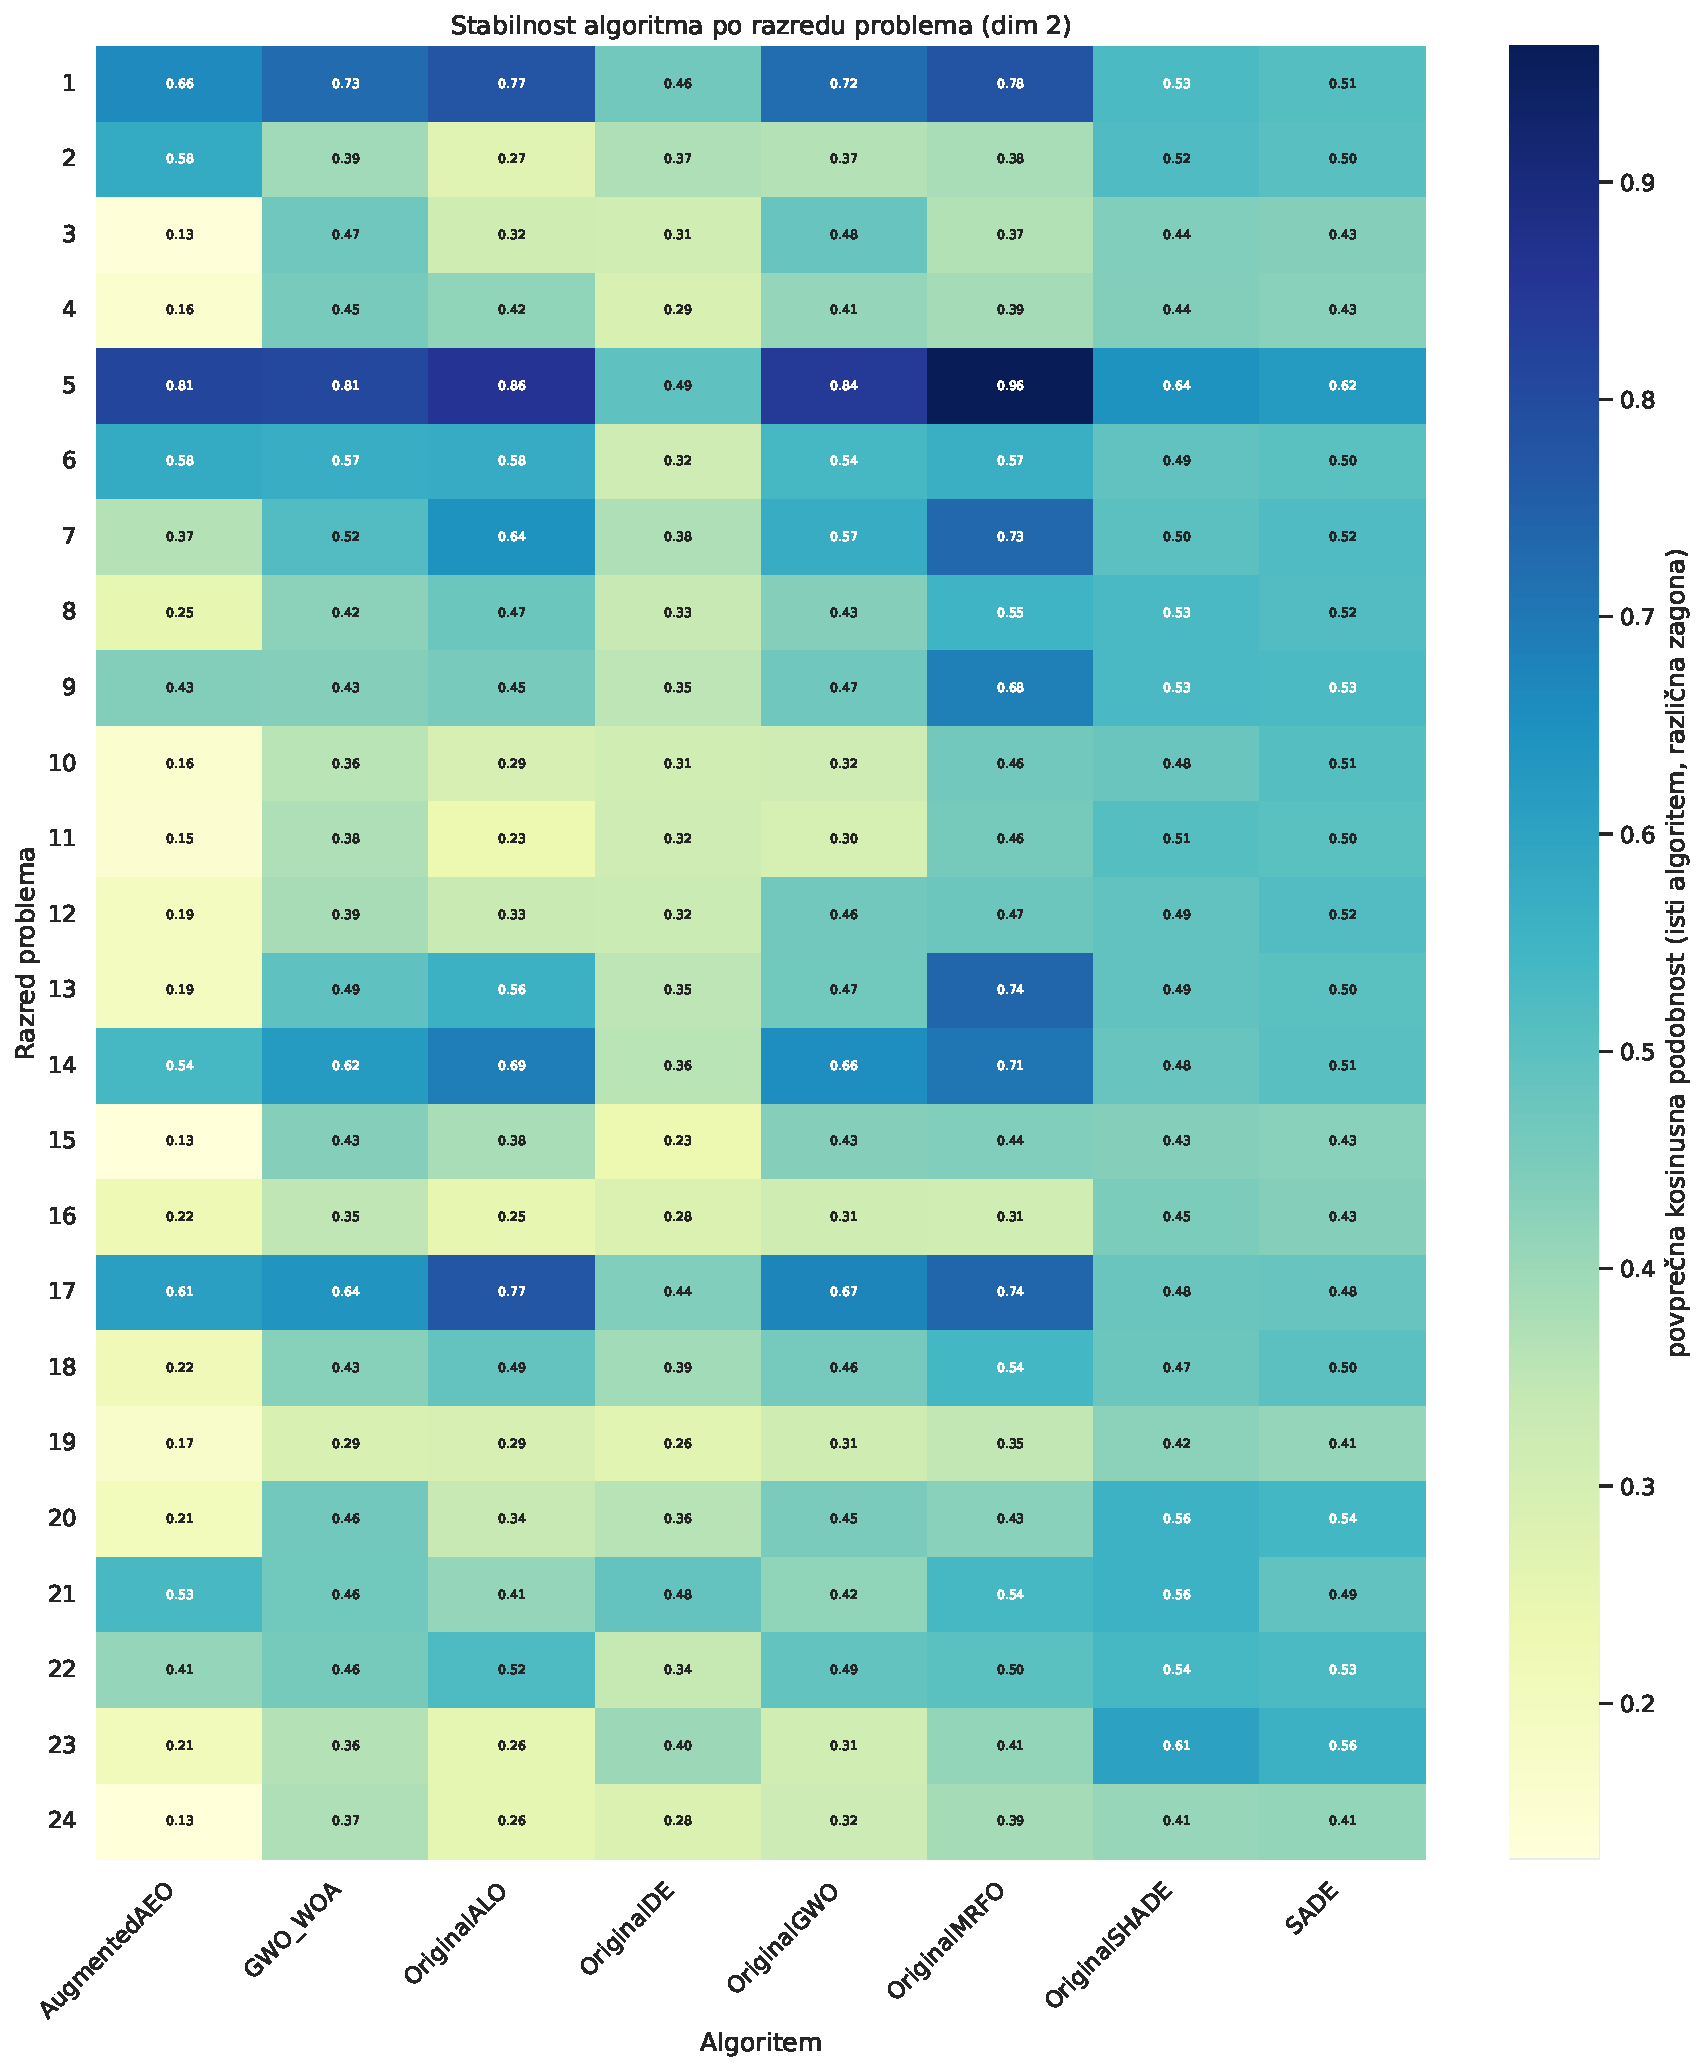
\includegraphics[width=\textwidth]{Slike/Diploma_slike/algorithm_similarity_per_problem_dim_2_scale_False.pdf}
        \caption{dimenzija 2}
        \label{fig:stabilnost-dim2}
    \end{subfigure}
    \hfill
    \begin{subfigure}[b]{0.48\textwidth}
        \centering
        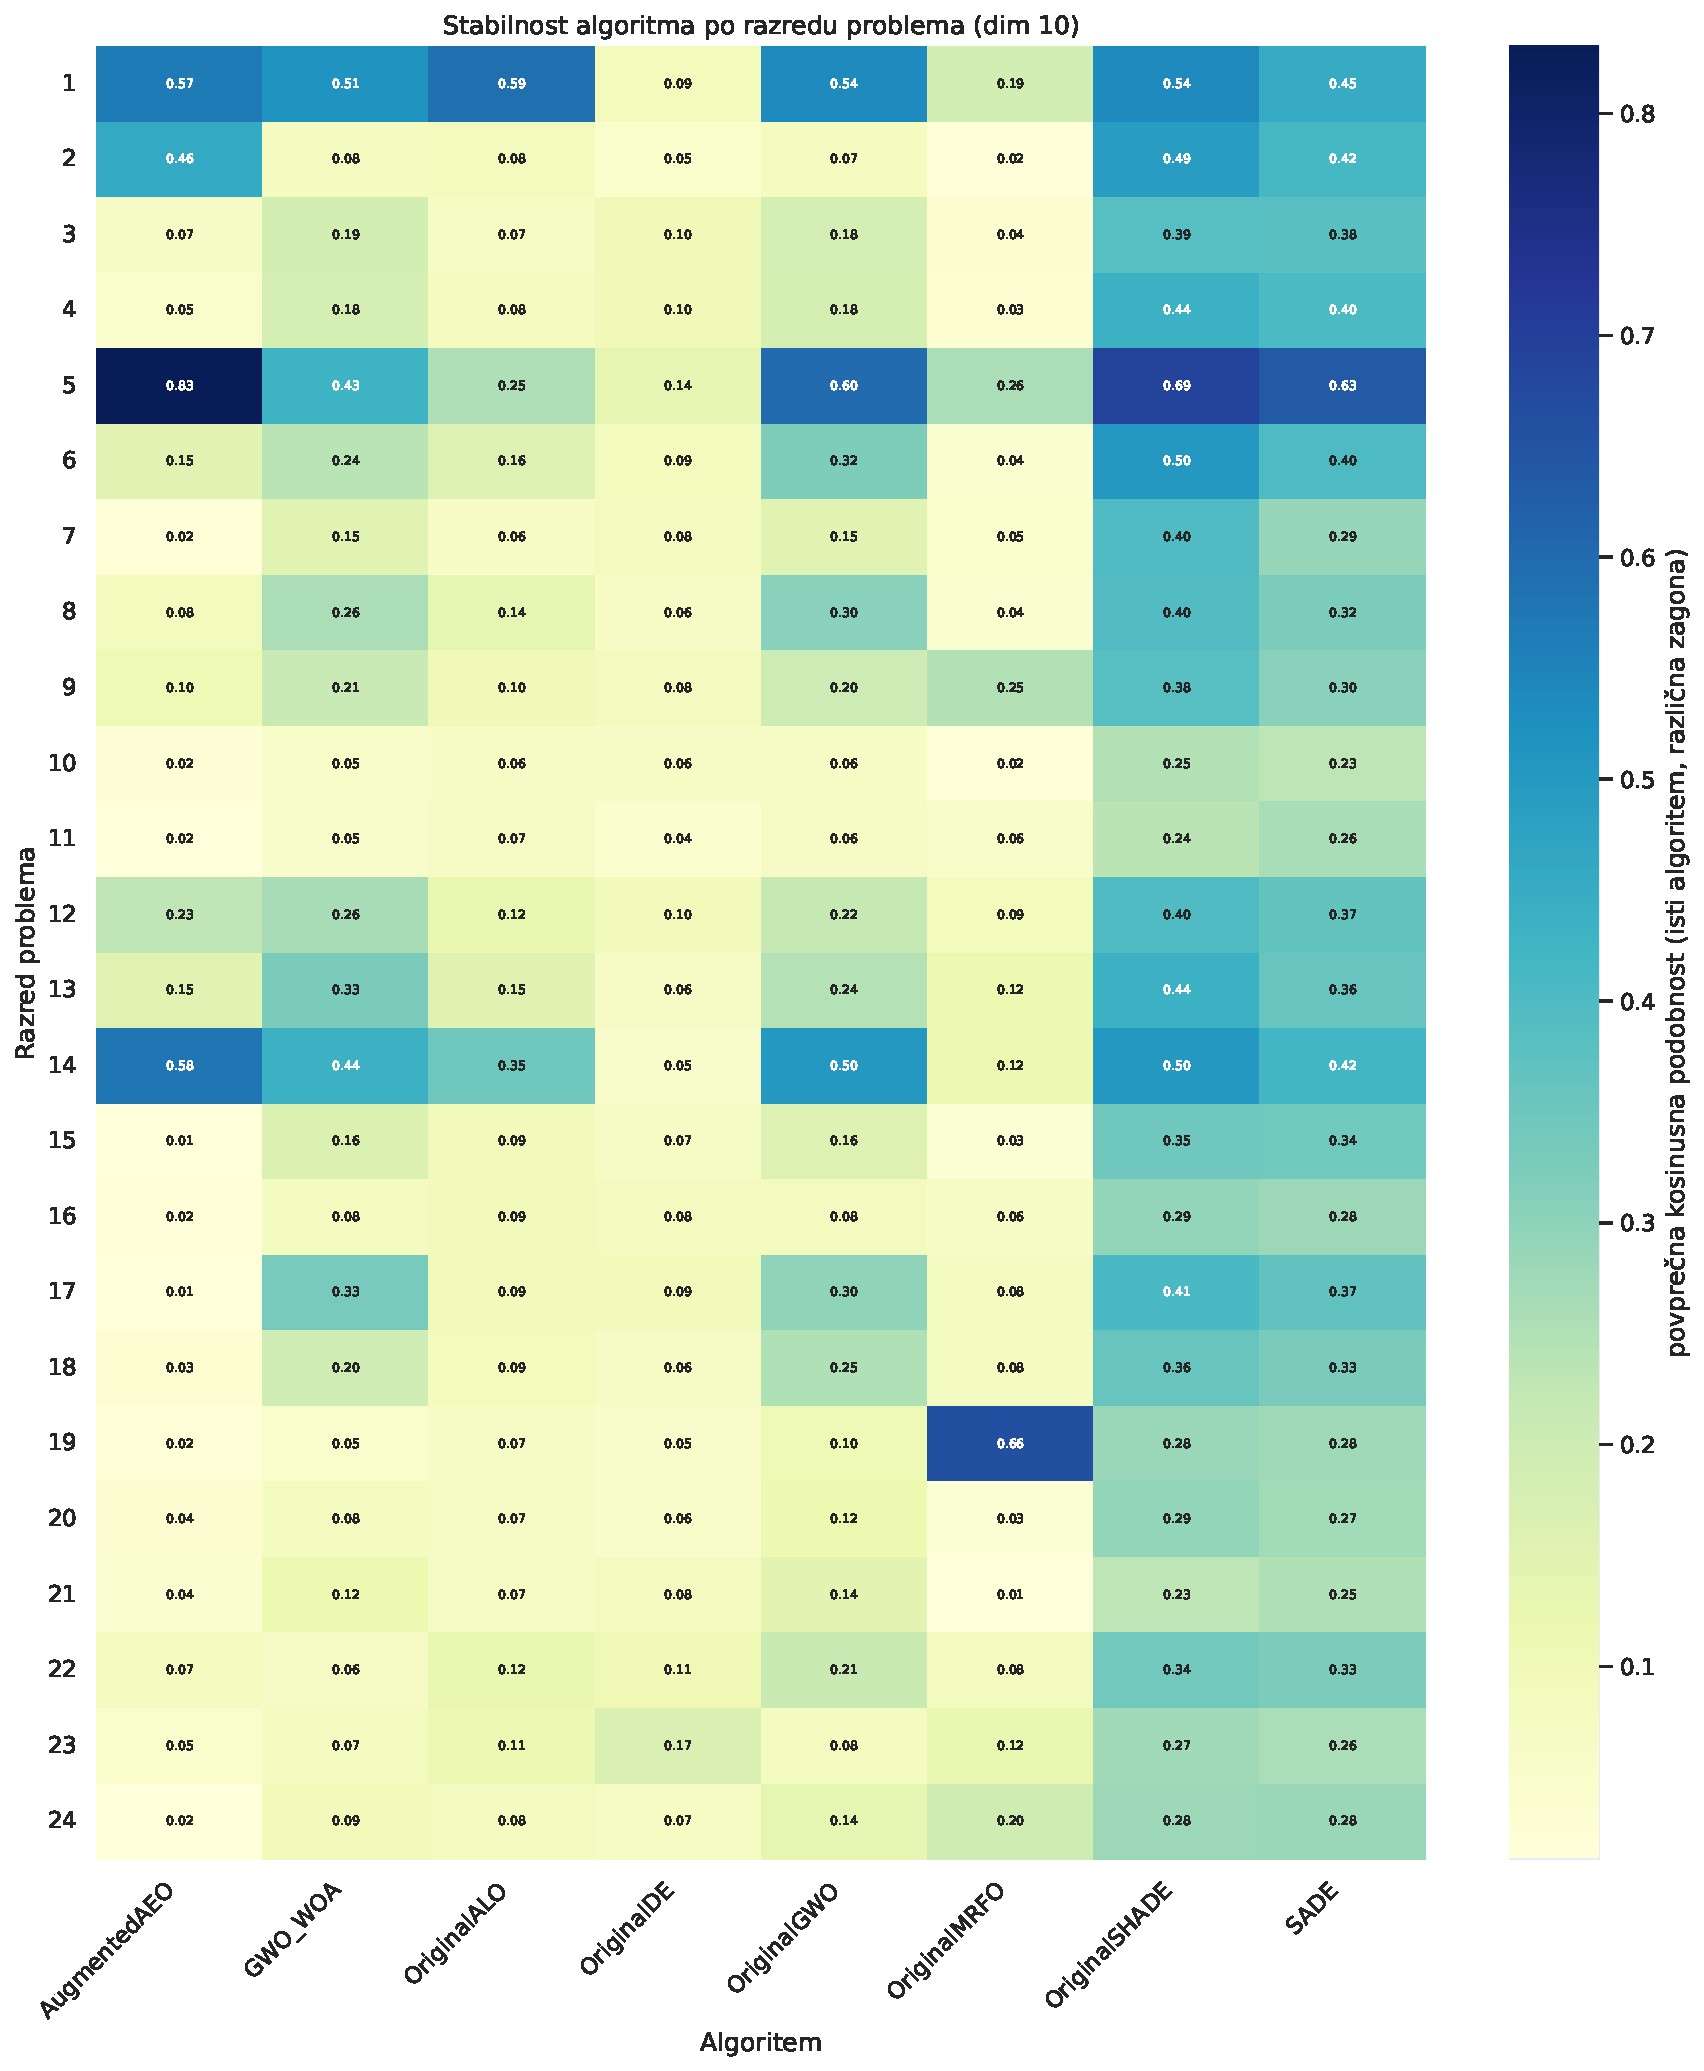
\includegraphics[width=\textwidth]{Slike/Diploma_slike/algorithm_similarity_per_problem_dim_10_scale_False.pdf}
        \caption{dimenzija 10}
        \label{fig:stabilnost-dim10}
    \end{subfigure}
    \caption{Stabilnost algoritmov glede na inicializacijo, agregirana po
    razredu problema, za dimenziji 2 (levo) in 10 (desno).}
    \label{fig:stabilnost-dim2-10}
\end{figure}

Nižja stabilnost v dimenziji 10 je skladna s pričakovanji glede na
naraščajočo velikost iskalnega prostora, saj populacija ostaja enako velika (50 agentov), zato ta
vsakič pokrije sorazmerno manjši del prostora in je vedenje algoritma bolj
odvisno od naključne inicializacije. K nižji izmerjeni stabilnosti 
delno prispeva tudi večje število gruč $k$, ki ga v višjih dimenzijah
pogosto izbere metoda komolca.

\section{Komplementarnost mer (Spearmanova korelacija)}
\label{sec:spearman}

To je osrednji rezultat, ki podpira tezo, da predlagane mere podobnosti
dajejo dejanski vpogled v vedenje algoritmov. Če bi bile med seboj močno
korelirane, bi večina njih le podvajala informacijo, ki jo že zajame ena
sama. Če so med seboj razmeroma neodvisne, vsaka prispeva svoj, dodaten
vidik. V tem razdelku to preverimo formalno, s Spearmanovo korelacijo med
vsemi pari mer.

\begin{definicija}[Spearmanov korelacijski koeficient]
\label{def:spearman}
Naj bosta $X = (x_1, \dots, x_n)$ in $Y = (y_1, \dots, y_n)$ vzorca $n$
opazovanj po parih, in naj $\mathrm{rang}(x_i)$ oziroma $\mathrm{rang}(y_i)$
označuje rang $i$-tega opazovanja znotraj vzorca $X$ oziroma $Y$ (najmanjša
vrednost ima rang 1). Spearmanov korelacijski koeficient je Pearsonov
korelacijski koeficient, izračunan na rangih:
\[
    \rho = \frac{\sum_{i=1}^n \bigl(\mathrm{rang}(x_i) - \overline{\mathrm{rang}(X)}\bigr)\bigl(\mathrm{rang}(y_i) - \overline{\mathrm{rang}(Y)}\bigr)}
    {\sqrt{\sum_{i=1}^n \bigl(\mathrm{rang}(x_i) - \overline{\mathrm{rang}(X)}\bigr)^2} \sqrt{\sum_{i=1}^n \bigl(\mathrm{rang}(y_i) - \overline{\mathrm{rang}(Y)}\bigr)^2}},
\]
kjer $\overline{\mathrm{rang}(X)}$ označuje povprečje rangov vzorca $X$.
Vrednost $\rho$ leži v intervalu $[-1, 1]$. Pri $\rho = 1$ gre za popolno
naraščajočo, pri $\rho = -1$ za popolno padajočo monotono povezanost, pri
$\rho = 0$ pa za odsotnost monotone povezanosti med $X$ in $Y$.
\end{definicija}

Spearmanovo korelacijo namesto Pearsonove uporabimo iz dveh razlogov.
Prvič, mere so med seboj na zelo različnih skalah. Štiri od njih
(entropija, obe kosinusni meri in razlika v raziskovanju) so omejene na
$[0,1]$, razliki v lokaciji in fitnessu pa sta neomejeni in se med
funkcijami razlikujeta za več velikostnih redov. Ker Spearmanova
korelacija namesto surovih vrednosti uporablja range, je neobčutljiva na
take razlike v skali. Drugič, zanima nas splošnejše vprašanje, ali dve meri
naraščata in padata skupaj (monotona povezanost), ne nujno po premici, kot
bi to zahtevala Pearsonova korelacija.

Jakost korelacije skozi to poglavje interpretiramo po lestvici, povzeti v
tabeli~\ref{tab:spearman-interpretacija}.

\begin{table}[H]
\centering
\begin{tabular}{@{}ll@{}}
\toprule
$|\rho|$ & Interpretacija \\
\midrule
$< 0{,}2$ & zanemarljiva \\
$0{,}2$--$0{,}4$ & šibka \\
$0{,}4$--$0{,}6$ & zmerna \\
$0{,}6$--$0{,}8$ & močna \\
$\ge 0{,}8$ & zelo močna \\
\bottomrule
\end{tabular}
\caption{Interpretacija velikosti Spearmanovega korelacijskega koeficienta,
uporabljena v tem poglavju.}
\label{tab:spearman-interpretacija}
\end{table}

V analizo vključimo šest mer, predstavljenih v
poglavju~\ref{ch:metrike}.
Za vsak par mer korelacijo izračunamo na vseh razpoložljivih parih
algoritmov, funkcij, instanc in zagonov znotraj posamezne dimenzije.
Slika~\ref{fig:spearman} prikazuje dobljene korelacijske matrike za
dimenzije 2, 5 in 10.


Iz matrik je razviden dosleden vzorec. Mere, ki izhajajo iz gručenja
trajektorij (entropija, kosinusna razdalja in kosinusna razdalja po gručah),
med seboj korelirajo zmerno (na primer korelacija med globalno in po
gručah kosinusno razdaljo znaša $\rho \approx 0{,}5$ v vseh treh dimenzijah), kar je pričakovano, saj izhajajo iz istega vira podatkov, a
kljub temu niso redundantne. Mere, ki izhajajo iz drugih virov podatkov, so
bolj neodvisne. Razlika v lokaciji in razlika v fitnessu korelirata močno
pri dimenziji 2 ($\rho = 0{,}69$), a ta povezava z dimenzijo hitro upade
(razdelek~\ref{sec:dimenzije}). Izjema je par entropija in razlika v
raziskovanju, ki kljub neodvisnemu izvoru izračuna korelira
zelo močno in z dimenzijo še narašča ($\rho = 0{,}77$ do $0{,}84$). 

\begin{figure}[H]
    \centering
    \begin{subfigure}[b]{\textwidth}
        \centering
        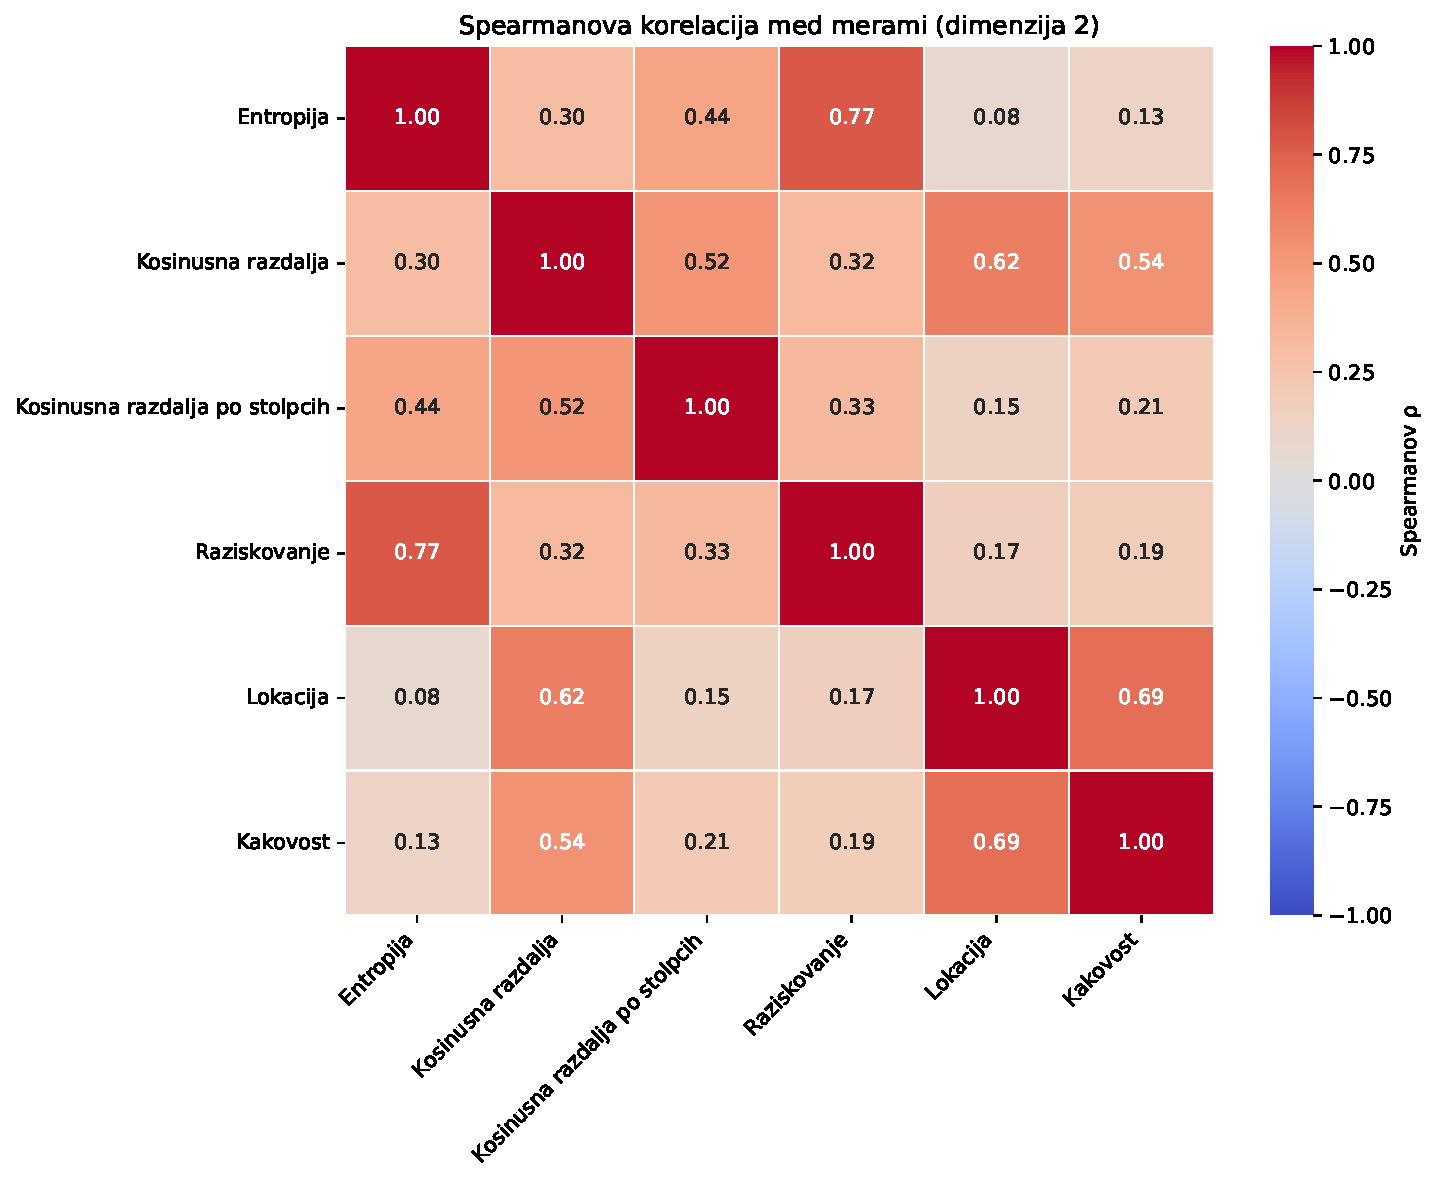
\includegraphics[width=\textwidth, height=0.245\textheight, keepaspectratio]{Slike/Diploma_slike/spearman_dim_2.pdf}
        \caption{Dimenzija 2}
        \label{fig:spearman-dim2}
    \end{subfigure}

    \vspace{0.5em}

    \begin{subfigure}[b]{\textwidth}
        \centering
        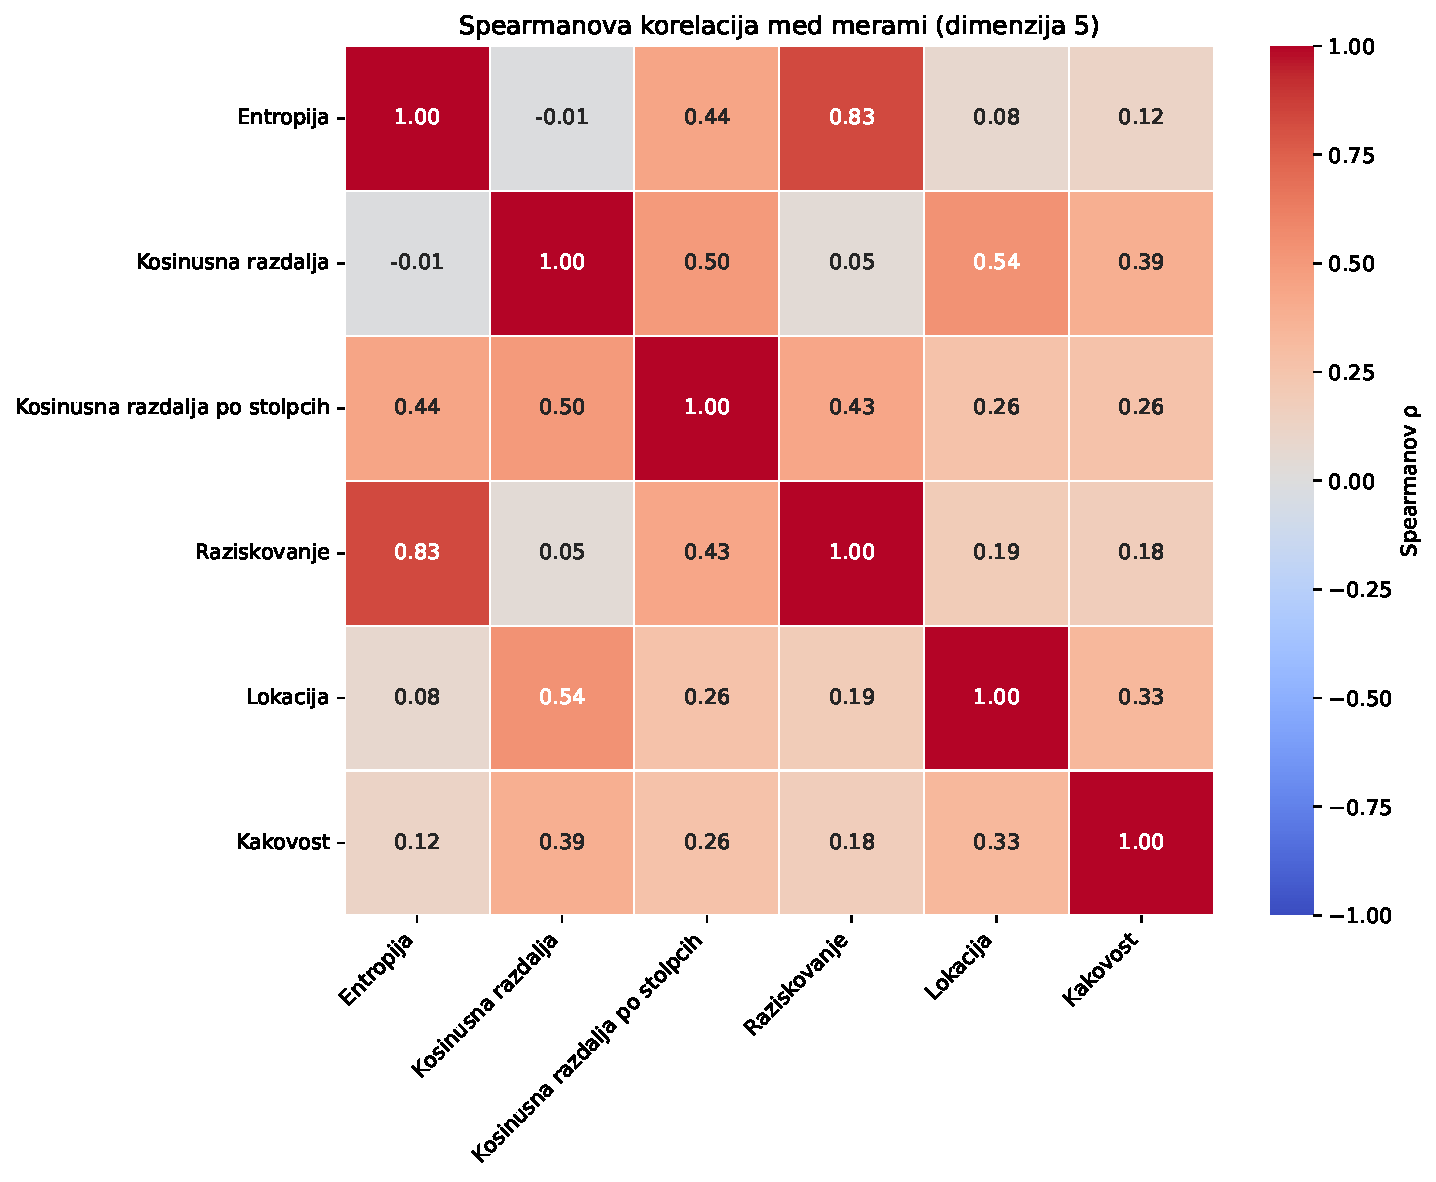
\includegraphics[width=\textwidth, height=0.245\textheight, keepaspectratio]{Slike/Diploma_slike/spearman_dim_5.pdf}
        \caption{Dimenzija 5}
        \label{fig:spearman-dim5}
    \end{subfigure}

    \vspace{0.5em}

    \begin{subfigure}[b]{\textwidth}
        \centering
        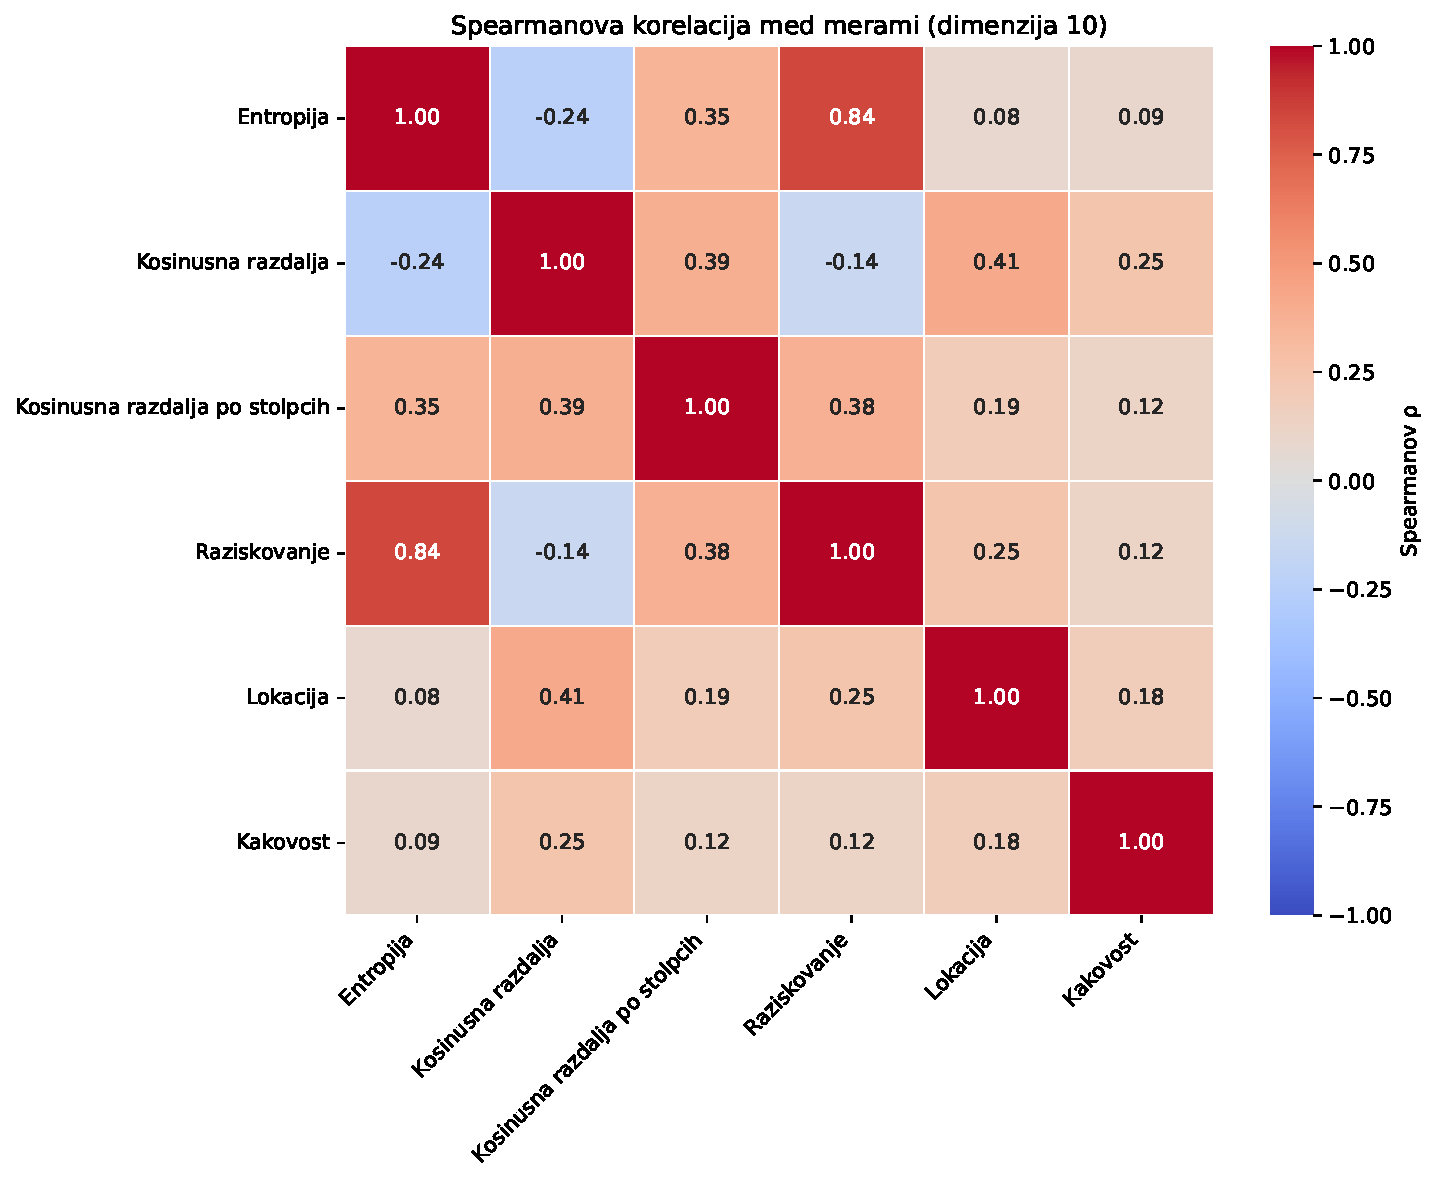
\includegraphics[width=\textwidth, height=0.245\textheight, keepaspectratio]{Slike/Diploma_slike/spearman_dim_10.pdf}
        \caption{Dimenzija 10}
        \label{fig:spearman-dim10}
    \end{subfigure}

    \caption{Spearmanova korelacija med šestimi merami podobnosti, ločeno po
    dimenzijah.}
    \label{fig:spearman}
\end{figure}


 
\section{Lokacija in fitness čez dimenzije}
\label{sec:dimenzije}

Mera razlike v lokaciji (razdelek~\ref{sec:location}) in mera razlike v
fitnessu (razdelek~\ref{sec:fitness}) merita navidez ločena vidika. Prva
pove, kako daleč narazen sta v iskalnem prostoru pristali končni rešitvi
dveh algoritmov, druga pa, kako različno kakovostni sta ti rešitvi.
Vprašanje, ki si ga zastavimo v tem razdelku, je, ali sta ta dva vidika med seboj povezana, in če, kako se ta povezava spreminja z naraščajočo
dimenzijo iskalnega prostora.

V nizko-dimenzionalnih, pogosto skoraj unimodalnih krajinah je odgovor
intuitiven. Če obstaja v bistvu en sam privlačni bazen, bližina končne
lokacije optimumu neposredno določa kakovost dosežene rešitve, zato
pričakujemo, da se mera razlike v lokaciji in mera razlike v fitnessu
ujemata. Z naraščajočo dimenzijo pa krajine praviloma postanejo bolj
multimodalne, kar algoritmoma omogoči, da dosežeta primerljivo kakovostni
rešitvi (nizka razlika v fitnessu), čeprav sta pristala v povsem različnih,
oddaljenih bazenih (visoka razlika v lokaciji). Vedenje se tako razklopi
od izida.

To hipotezo potrdi Spearmanova korelacija med merama razlike v lokaciji in
razlike v fitnessu (glej razdelek~\ref{sec:spearman}), ki z naraščajočo
dimenzijo dosledno upada in znaša $\rho = 0{,}69$ pri dimenziji 2, $\rho = 0{,}33$
pri dimenziji 5 in $\rho = 0{,}18$ pri dimenziji 10. Upad je monoton in izrazit, od močne povezanosti pri dimenziji 2 do zanemarljive pri dimenziji 10, kar je skladno s tem, da krajine z naraščajočo dimenzijo
iskalnega prostora postajajo vse bolj zapletene.

Isti pojav si od blizu oglejmo še na enem samem, izrazito multimodalnem
problemu ($\prob{21}{1}$), kjer namesto rangov uporabimo surove vrednosti obeh
mer, saj znotraj enega problema mešanje skal med funkcijami ni prisotno.
Slika~\ref{fig:lokacija-fitness-scatter} prikazuje vse pare med 28
algoritmi na tem problemu (torej $\binom{28}{2} = 378$ točk),
ločeno po dimenziji, skupaj z regresijsko premico.


\begin{figure}[H]
    \centering
    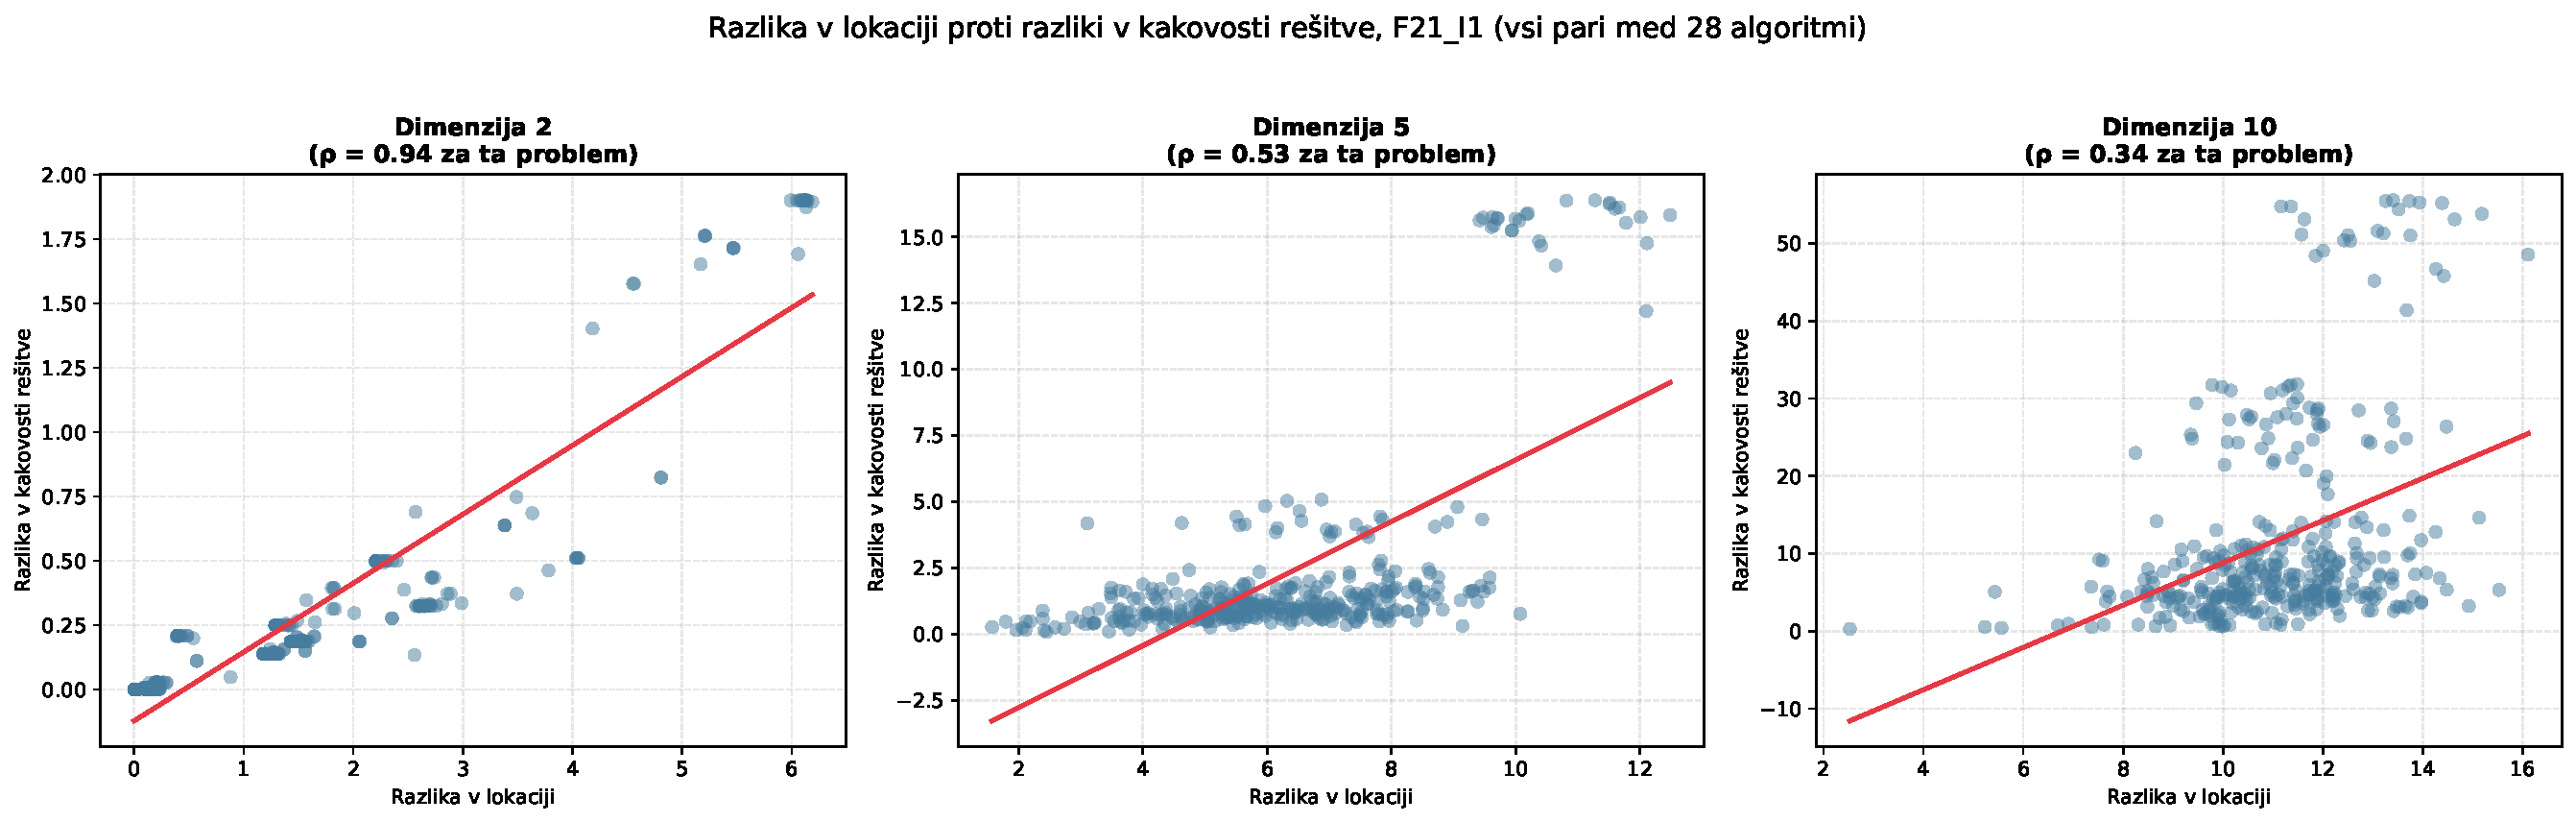
\includegraphics[width=\textwidth]{Slike/Diploma_slike/lokacija_fitness_scatter_F21_I1.pdf}
    \caption{Razlika v lokaciji proti razliki v fitnessu za vse pare. Spearmanova
    korelacija na tem problemu ($\rho = 0{,}94$ pri dimenziji 2,
    $\rho = 0{,}53$ pri dimenziji 5, $\rho = 0{,}34$ pri dimenziji 10) sledi
    istemu padajočemu trendu kot agregatna korelacija čez vse obravnavane
    probleme, a je na tem posameznem, izrazito multimodalnem problemu še
    bolj izrazita.}
    \label{fig:lokacija-fitness-scatter}
\end{figure}


\section{Konvergentna veljavnost: entropija in raziskovanje}
\label{sec:konvergenca}

Entropija zasedenosti gruč (razdelek~\ref{sec:entropy}) in razlika v
raziskovanju/izkoriščanju (razdelek~\ref{sec:exploration}) izhajata iz
\emph{popolnoma neodvisnih} virov podatkov. Prva izhaja iz gručenja populacijskih
trajektorij, druga iz notranje mere razpršenosti, ki jo med reševanjem
neodvisno beleži knjižnica mealpy. Kljub temu obe intuitivno merita isto osnovno lastnost, razpršenost populacije po iskalnem prostoru skozi čas, le prek povsem različnih poti izračuna.

Če se meri kljub neodvisnima izvoroma ujemata, to ni posledica skupnega
vira podatkov (ker ga ni), temveč dokaz, da obe dejansko merita to, kar trdita, t.\,i.\ \emph{konvergentna veljavnost}. Spearmanova korelacija
med tema dvema meroma (glej razdelek~\ref{sec:spearman}) je visoka skozi
vse tri dimenzije in z dimenzijo celo rahlo narašča in znaša $\rho = 0{,}77$ pri
dimenziji 2, $\rho = 0{,}83$ pri dimenziji 5 in $\rho = 0{,}84$ pri
dimenziji 10. Gre za natanko nasproten vzorec od tistega, ki smo ga opazili
med lokacijo in fitnessom v razdelku~\ref{sec:dimenzije}. Medtem ko se tam
povezava z naraščajočo dimenzijo razklopi, tu ostane trdno prisotna in se
še okrepi.

Vrednosti pri dimenzijah 5 in 10 sicer presegajo prag, ki bi ga sicer brali
kot znak redundance med merama. Vendar velja opozoriti, da je taka
interpretacija smiselna predvsem takrat, kadar meri delita skupen vir
podatkov (kot na primer obe kosinusni meri, ki obe izhajata iz gručenja). Tam bi visoka korelacija dejansko pomenila, da ena mera drugi ne doda nič
novega. Pri entropiji in raziskovanju pa visoka korelacija kaže na obratno. Obe neodvisno zaznata isto lastnost
vedenja algoritmov.


Slika~\ref{fig:entropija-raziskovanje-f23} ponazori to ujemanje na
konkretnem primeru. Algoritmi, ki v entropijski krivulji
(slika~\ref{fig:entropija-f23}) hitro konvergirajo, enako hitro konvergirajo
tudi v deležu raziskovanja (slika~\ref{fig:raziskovanje-f23}), in obratno za
tiste, ki ostanejo razpršeni skozi ves zagon.


\begin{figure}[H]
    \centering
    \begin{subfigure}[b]{0.85\textwidth}
        \centering
        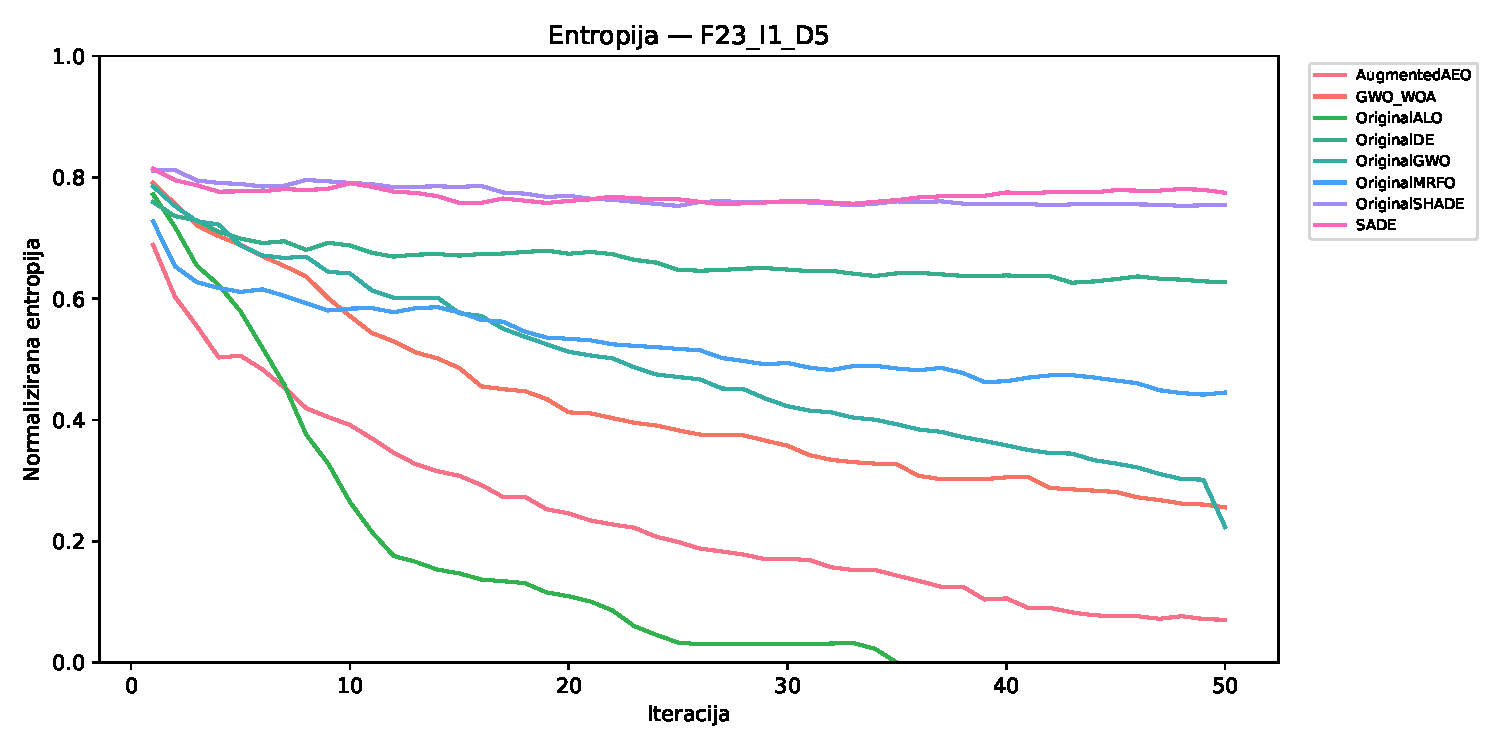
\includegraphics[width=\textwidth]{Slike/Diploma_slike/entropija_F23_I1_D5.pdf}
        \caption{Normalizirana entropija}
        \label{fig:entropija-f23}
    \end{subfigure}

    \vspace{1em}

    \begin{subfigure}[b]{0.85\textwidth}
        \centering
        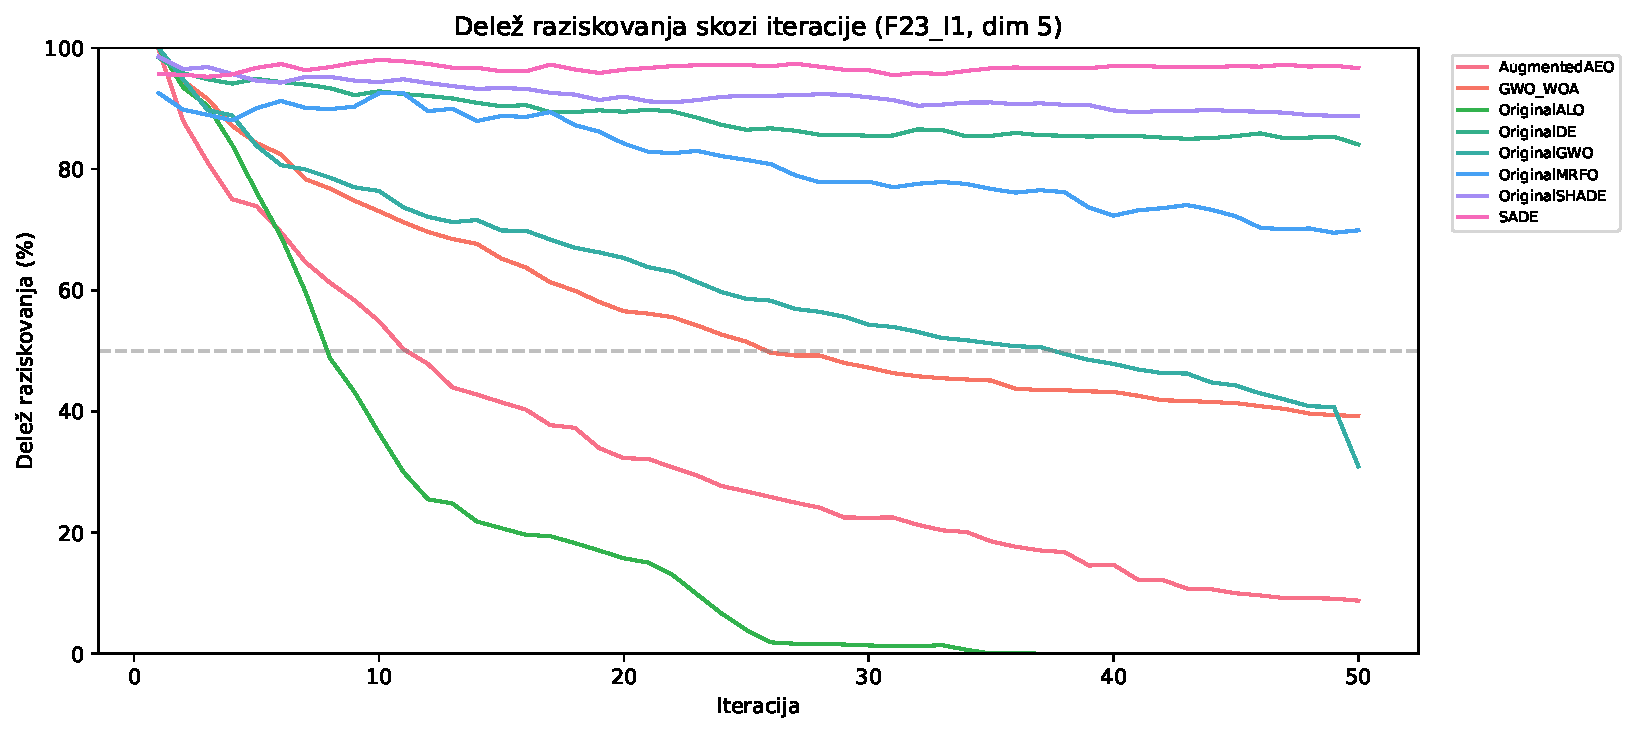
\includegraphics[width=\textwidth]{Slike/Diploma_slike/mean_exploration_exploitation_F23_I1_dim5.pdf}
        \caption{Delež raziskovanja}
        \label{fig:raziskovanje-f23}
    \end{subfigure}
    \caption{Normalizirana entropija (zgoraj) in delež raziskovanja (spodaj)
    skozi iteracije, za isto množico algoritmov na problemu $\prob{23}{1}$,
    dimenzija 5, z enako barvno shemo na obeh slikah.}
    \label{fig:entropija-raziskovanje-f23}
\end{figure}

\section{Entropija skozi probleme in dimenzije}
\label{sec:entropija-fitness}

\subsection{Entropija in fitness na enem problemu}

Dimenzijski razklop iz razdelka~\ref{sec:dimenzije} si oglejmo še na ravni
posameznih algoritmov, na istem problemu ($\prob{21}{1}$) v dimenzijah 2 in 10.
Slika~\ref{fig:entropija-fitness-f21} prikazuje normalizirano entropijo
skozi iteracije za osem algoritmov, z legendo, urejeno po končnem
fitnessu (najboljši prvi), ki poleg fitnessa navaja tudi razliko do
pravega optimuma $\Delta$, evklidsko razdaljo do optimuma $d$ in končno
entropijo $H_{\text{konec}}$.

Pri dimenziji 2 (slika~\ref{fig:entropija-fitness-f21}a) je fitness med
vsemi osmimi algoritmi skoraj identičen ($40{,}8$--$41{,}1$, $\Delta$ med
$2{,}5 \cdot 10^{-9}$ in $0{,}32$), kljub temu da se končna entropija giblje
od popolnega kolapsa ($H_{\text{konec}} = 0{,}00$ pri OriginalDE,
AugmentedAEO, OriginalALO in OriginalGWO) do skoraj nespremenjene
razpršenosti ($H_{\text{konec}} = 0{,}72$ pri OriginalSHADE). Celo razdalja
do pravega optimuma se giblje od $0{,}00$ do $2{,}61$, fitness pa ostane praktično raven, nazoren primer razklopa vedenja od izida, ki smo ga
kvantitativno pokazali v razdelku~\ref{sec:dimenzije}.

Pri dimenziji 10 (slika~\ref{fig:entropija-fitness-f21}b) je slika
drugačna. Fitness se med algoritmi opazno razlikuje ($42{,}4$--$51{,}0$,
$\Delta$ med $1{,}6$ in $10{,}0$, torej za red velikosti večji razpon kot
pri dimenziji 2). Zanimivo pa je, da je kar šest od osmih algoritmov
doseglo popoln kolaps entropije ($H_{\text{konec}} = 0{,}00$), a kljub temu
dosegajo zelo različno kakovostne rešitve. To pomeni, da sam kolaps
entropije ne napove kakovosti dosežene rešitve. Odločilno je, kam
je populacija konvergirala, ne le, ali je. Omembe vredno je tudi, da sta
edina algoritma, ki nista popolnoma konvergirala
($H_{\text{konec}} \approx 0{,}2$ pri OriginalSHADE in SADE), hkrati tudi najboljša po fitnessu. Na tako majhnem vzorcu tega sicer ne moremo
posplošiti v splošno pravilo, je pa skladno z ugotovitvijo iz
razdelka~\ref{sec:konvergenca}, da je ohranjanje raziskovanja povezano z
razpršenostjo populacije skozi celoten zagon.

Možna razlaga tega vzorca je vezana na naravo problema $F_{21}$, ki spada med
multimodalne funkcije s šibko globalno strukturo (razdelek~\ref{sec:bbob})
in ima izjemno veliko lokalnih minimumov. Algoritem, ki entropijo zniža
hitro, se v bistvu zaveže naključnemu izmed teh mnogih bazenov, še preden
je prostor smiselno raziskal. Kakovost tako dosežene rešitve je zato
močno odvisna od sreče pri izbiri začetne smeri. Algoritem, ki entropijo
znižuje postopno, kot to počneta OriginalSHADE in SADE, po drugi strani
dlje ohranja možnost, da najde ugodnejši bazen, preden se dokončno usmeri vanj, pri dimenziji 10 pa ima za to na voljo bistveno več iteracij kot pri
dimenziji 2, saj število iteracij v tem delu narašča premo sorazmerno z
dimenzijo (razdelek~\ref{sec:mc}). Ta razlaga je verjetno v veliki meri
odvisna od lastnosti konkretnega problema. Pri manj multimodalnih
funkcijah bi bila prednost postopne konvergence lahko manj izrazita ali
odsotna.

\begin{figure}[H]
    \centering
    \begin{subfigure}[b]{\textwidth}
        \centering
        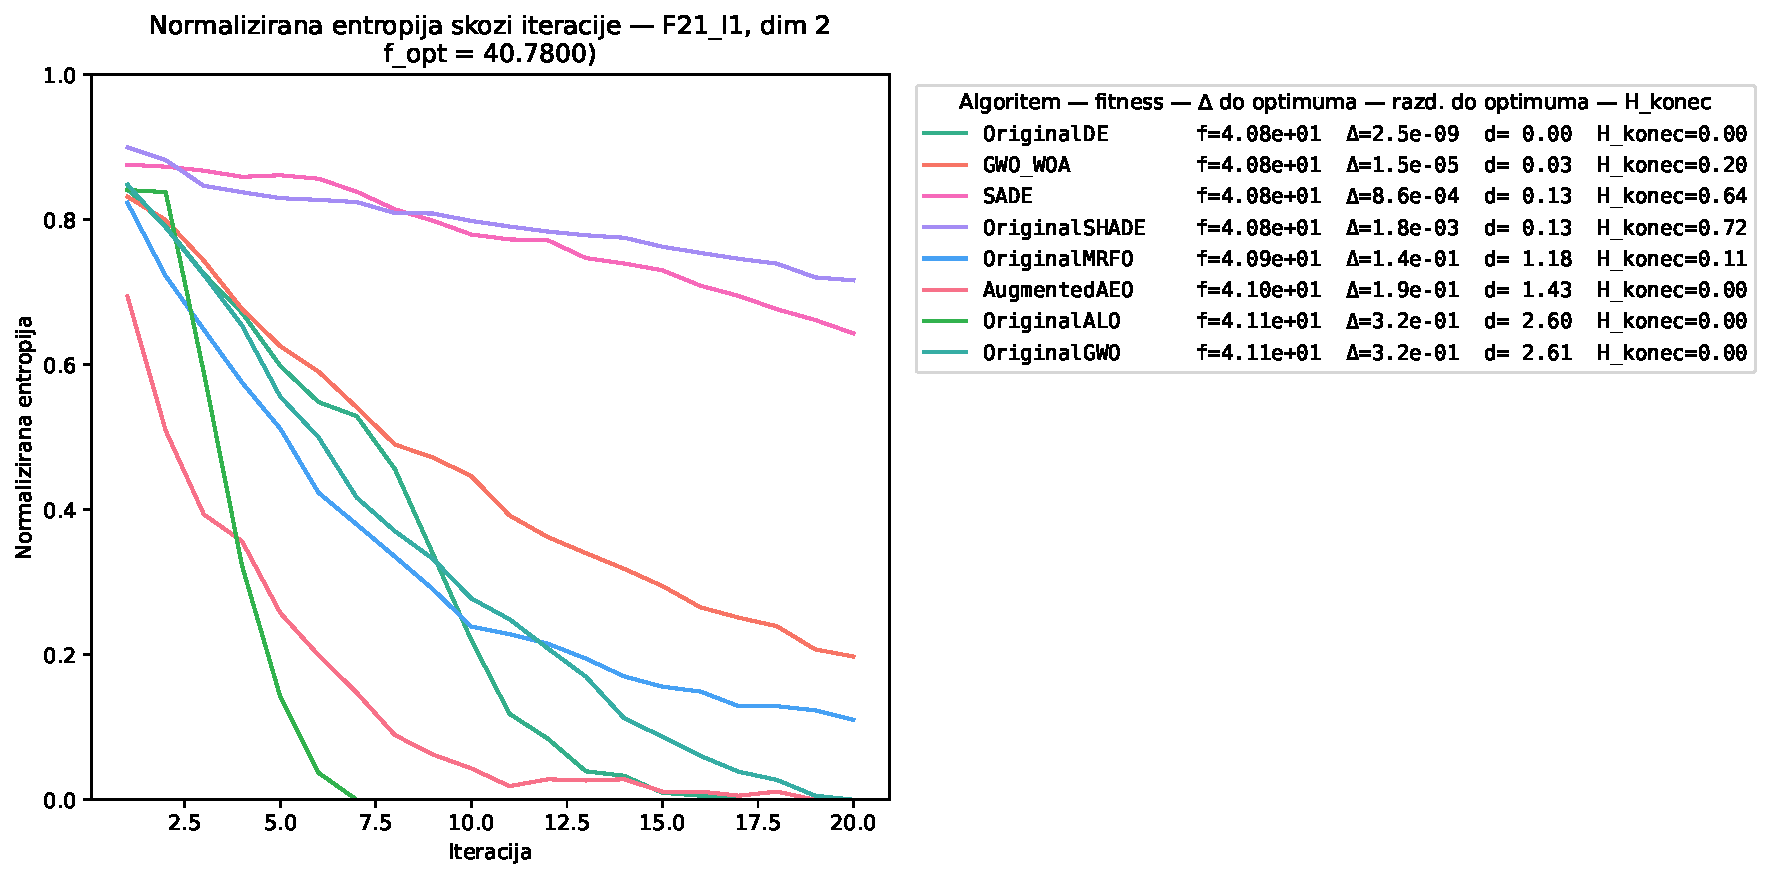
\includegraphics[width=\textwidth]{Slike/Diploma_slike/entropy_fitness_F21_I1_dim2_loc.pdf}
        \caption{Dimenzija 2}
        \label{fig:entropija-fitness-f21-dim2}
    \end{subfigure}

    \vspace{1em}

    \begin{subfigure}[b]{\textwidth}
        \centering
        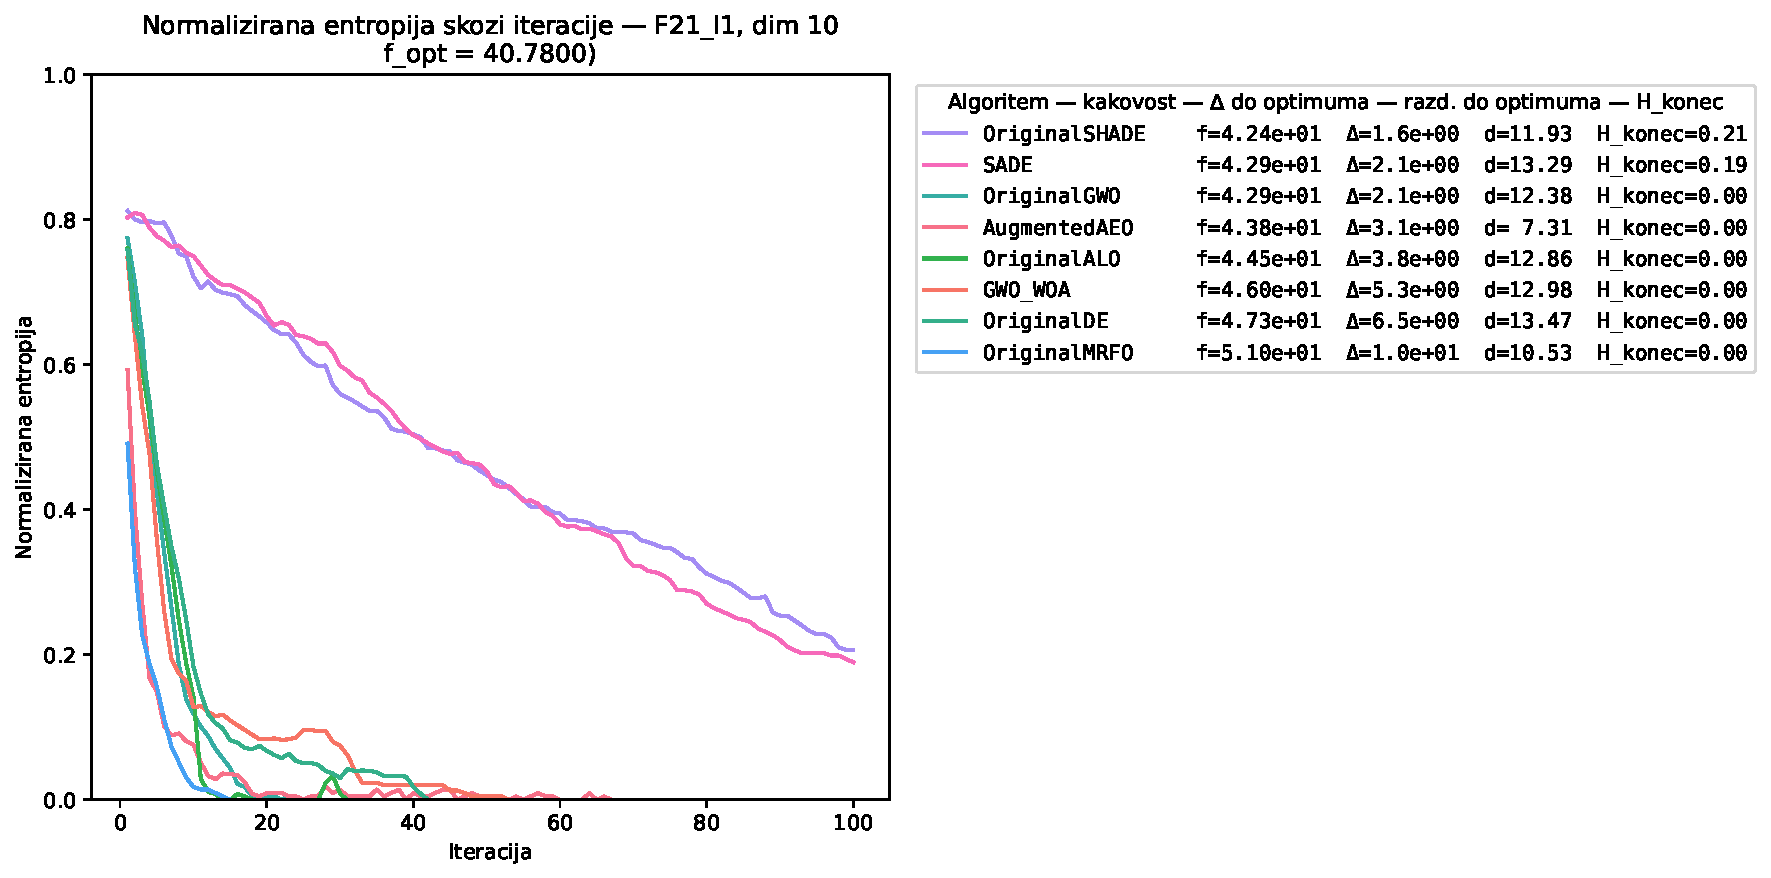
\includegraphics[width=\textwidth]{Slike/Diploma_slike/entropy_fitness_F21_I1_dim10_loc.pdf}
        \caption{Dimenzija 10}
        \label{fig:entropija-fitness-f21-dim10}
    \end{subfigure}
    \caption{Normalizirana entropija skozi iteracije na problemu $\prob{21}{1}$, v
    dimenziji 2 (zgoraj) in dimenziji 10 (spodaj). Legenda je urejena po
    končnem fitnessu (padajoče) in navaja fitness, razliko do
    optimuma $\Delta$, evklidsko razdaljo do optimuma $d$ ter končno
    entropijo $H_{\text{konec}}$.}
    \label{fig:entropija-fitness-f21}
\end{figure}

\subsection{Prilagodljivost glede na težavnost problema}

Zgornji primer obravnava en sam, težak problem. Da bi pokazali, kako se
entropijsko vedenje posameznega algoritma spreminja glede na težavnost
problema samega, primerjajmo štiri algoritme (OriginalAEO, OriginalALO,
OriginalGWO in SADE) na dveh nasprotnih si funkcijah nabora BBOB: $F_1$
(ločljiva, unimodalna, torej najpreprostejši problem v naboru) in $F_{23}$
(multimodalna s šibko globalno strukturo, med najzahtevnejšimi).
Slika~\ref{fig:entropija-uni-multi} prikazuje entropijske krivulje obeh
funkcij za vsak algoritem posebej, v vseh treh dimenzijah.
Algoritmi se glede na to primerjavo razlikujejo po tem, koliko svoje
vedenje \emph{prilagodijo} težavnosti problema. OriginalALO se na $F_1$ in
$F_{23}$ obnaša skoraj identično, v vseh treh dimenzijah entropijo hitro
zniža ne glede na to, ali je problem preprost ali zahteven. Njegovo vedenje
je tako rekoč neobčutljivo na težavnost problema. OriginalAEO nasprotno
dosledno loči med obema funkcijama. Na $F_1$ entropijo vselej hitro zniža,
na $F_{23}$ pa jo znižuje postopno, pri dimenziji 10 pa ostane nad $0{,}2$
skozi vseh 100 iteracij. Pri OriginalGWO je razlika med funkcijama izrazita
pri dimenzijah 2 in 5, pri dimenziji 10 pa se opazno zoži, saj tam entropijo
postopno znižuje na obeh funkcijah.
Najbolj skrajen primer prilagodljivosti kaže SADE. Na $F_1$ entropija dolgo
ostane visoka, nato pa \emph{nenadoma} pade, medtem ko na
$F_{23}$ pri dimenziji 10 entropija skozi celoten zagon ostane praktično
nespremenjena okoli vrednosti $0{,}7$. Algoritem se torej v danem
proračunu iteracij na tem problemu v bistvu ne zaveže nobeni rešitvi. To se
sklada z opažanjem iz prejšnjega razdelka, kjer je bil SADE eden od dveh
algoritmov, ki na $F_{21}$ pri dimenziji 10 nista popolnoma konvergirala proti kateri rešitvi.

\begin{figure}[H]
    \centering
    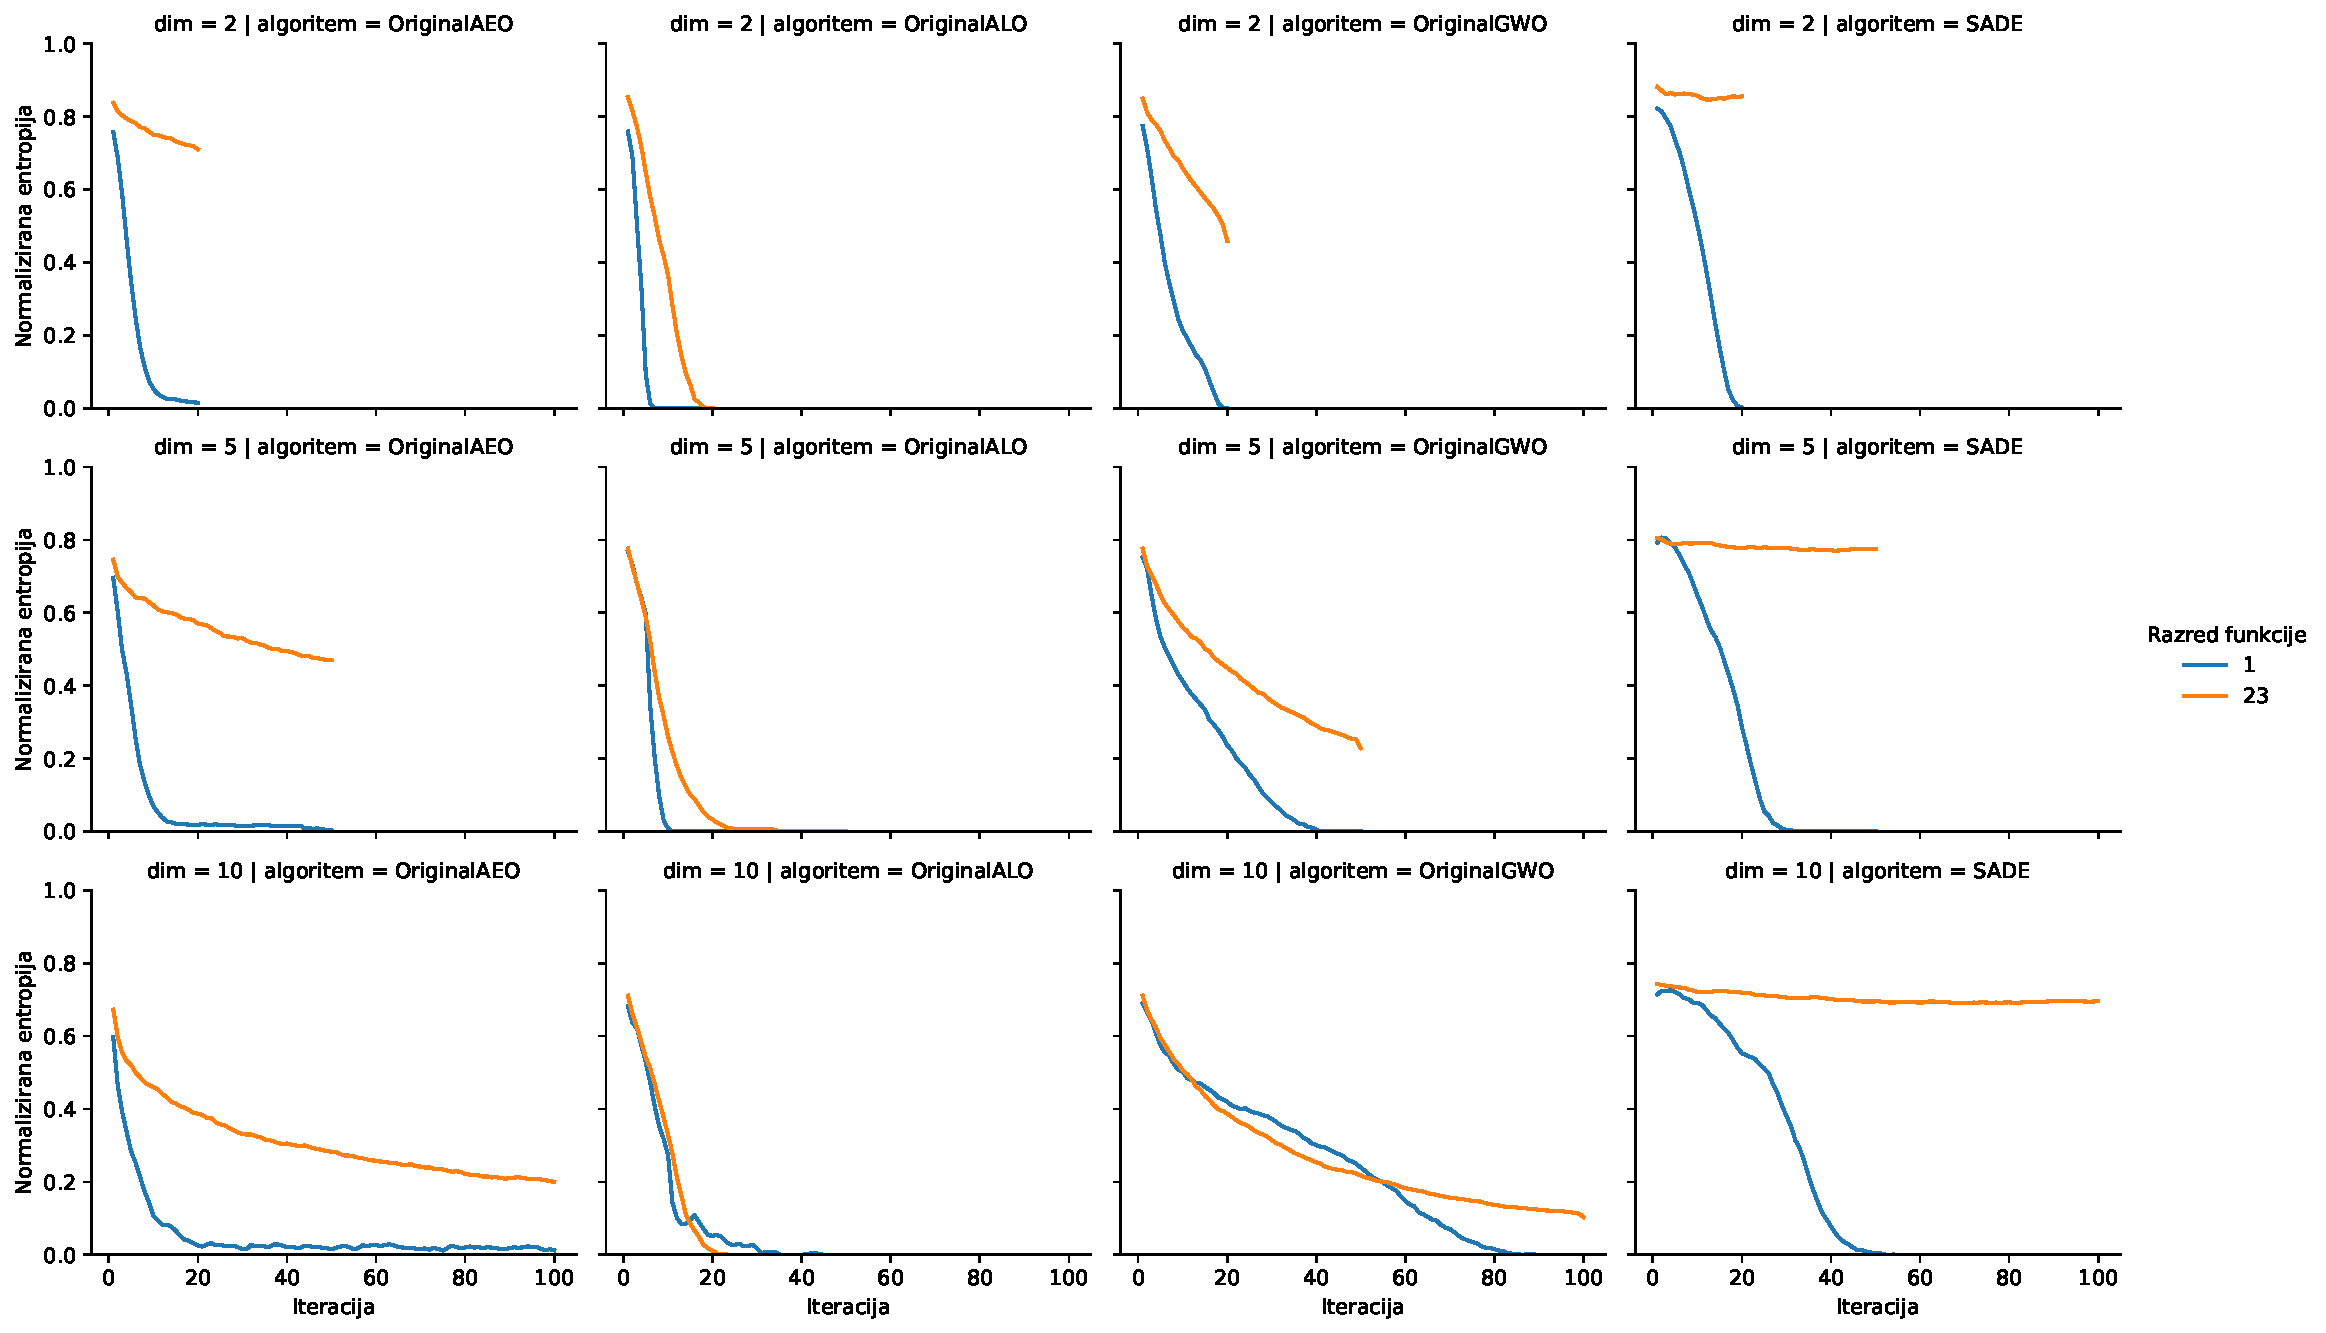
\includegraphics[width=\textwidth]{Slike/Diploma_slike/uni_vs_multimodal.pdf}
    \caption{Normalizirana entropija skozi iteracije na ločljivi, unimodalni
    funkciji $F_1$ (modro) in multimodalni funkciji s šibko globalno
    strukturo $F_{23}$ (oranžno), za štiri algoritme (stolpci) v treh
    dimenzijah (vrstice).}
    \label{fig:entropija-uni-multi}
\end{figure}


\section{Gručenje algoritmov po merah}
\label{sec:grucenje-metrike}
V tem razdelku preverimo komplementarnost mer na drugačen, vizualen način.
Namesto Spearmanove korelacije med samimi merami (razdelek~\ref{sec:spearman})
tu preverimo, ali se \emph{isti} algoritmi gručijo \emph{enako} ali
\emph{različno}, glede na to, katero mero uporabimo za primerjavo. Če se
neka skupina algoritmov (npr.\ družina DE) vselej gruči skupaj ne glede na
uporabljeno mero, to pomeni, da mere med njimi zaznavajo vedenjsko
sorodnost, ki ni le naključje posameznih meritev. Pri vseh treh dendrogramih
v tem razdelku uporabimo hierarhično gručenje z metodo \emph{povprečnega
povezovanja} (angl.\ average linkage), pri kateri je razdalja med dvema
skupinama povprečje razdalj med vsemi pari njunih elementov.
Slika~\ref{fig:grucenje-entropija} prikazuje gručenje na podlagi
entropijske krivulje. Dendrogram razkrije tri
jasno ločene skupine. OriginalSHADE in SADE nikoli zares ne konvergirata,
saj entropija ostane visoka skozi ves zagon. OriginalALO, AugmentedAEO,
OriginalAEO in OriginalMRFO hitro in popolnoma konvergirajo. OriginalDE,
GWO\_WOA in OriginalGWO prav tako hitro padejo, a se ustalijo na zmerni,
ne ničelni ravni. Razlog zakaj se \emph{OriginalDE} obnaša drugače kot \emph{OriginalSHADE} in \emph{SADE}, čeprav so vsi iz DE družine je to, da \emph{OriginalDE} nima nobenega mehanizma prilagajanja entropije populacije, medtem ko druga dva sta oba \sn{self-adapting} verzije, torej se s težavnostjo problema entropija njune populacije spreminja.
\begin{figure}[H]
    \centering
    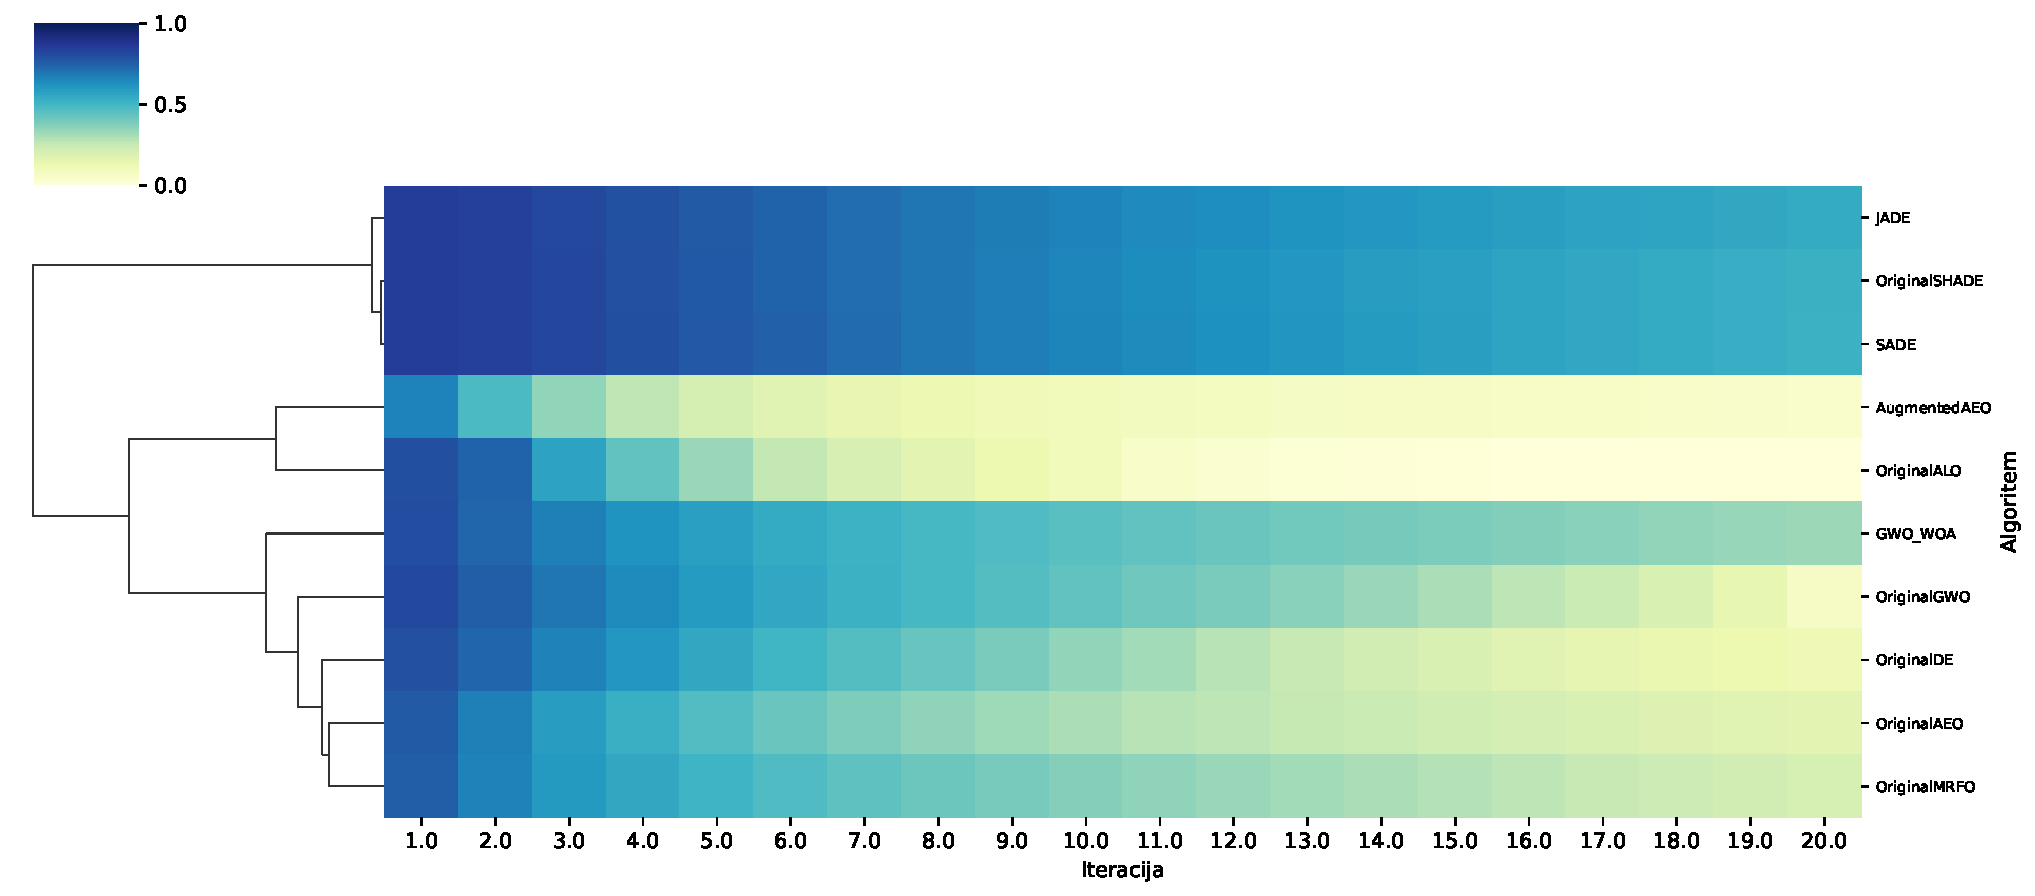
\includegraphics[width=\textwidth]{Slike/Diploma_slike/entropy_clustermap_dim2.pdf}
    \caption{Gručenje algoritmov na podlagi surove entropijske krivulje
    (matrika algoritem $\times$ iteracija), dimenzija 2.}
    \label{fig:grucenje-entropija}
\end{figure}
Slika~\ref{fig:grucenje-kosinusna} prikazuje gručenje na podlagi kosinusne
podobnosti, podedovane iz predhodnega dela (razdelek~\ref{sec:sorodna}). 
Tu se družina DE (SADE, JADE, OriginalSHADE) jasno združi, z medsebojno podobnostjo $0{,}49$--$0{,}50$, kar je precej več kot njena podobnost do AugmentedAEO ($0{,}17$--$0{,}20$).
\begin{figure}[H]
    \centering
    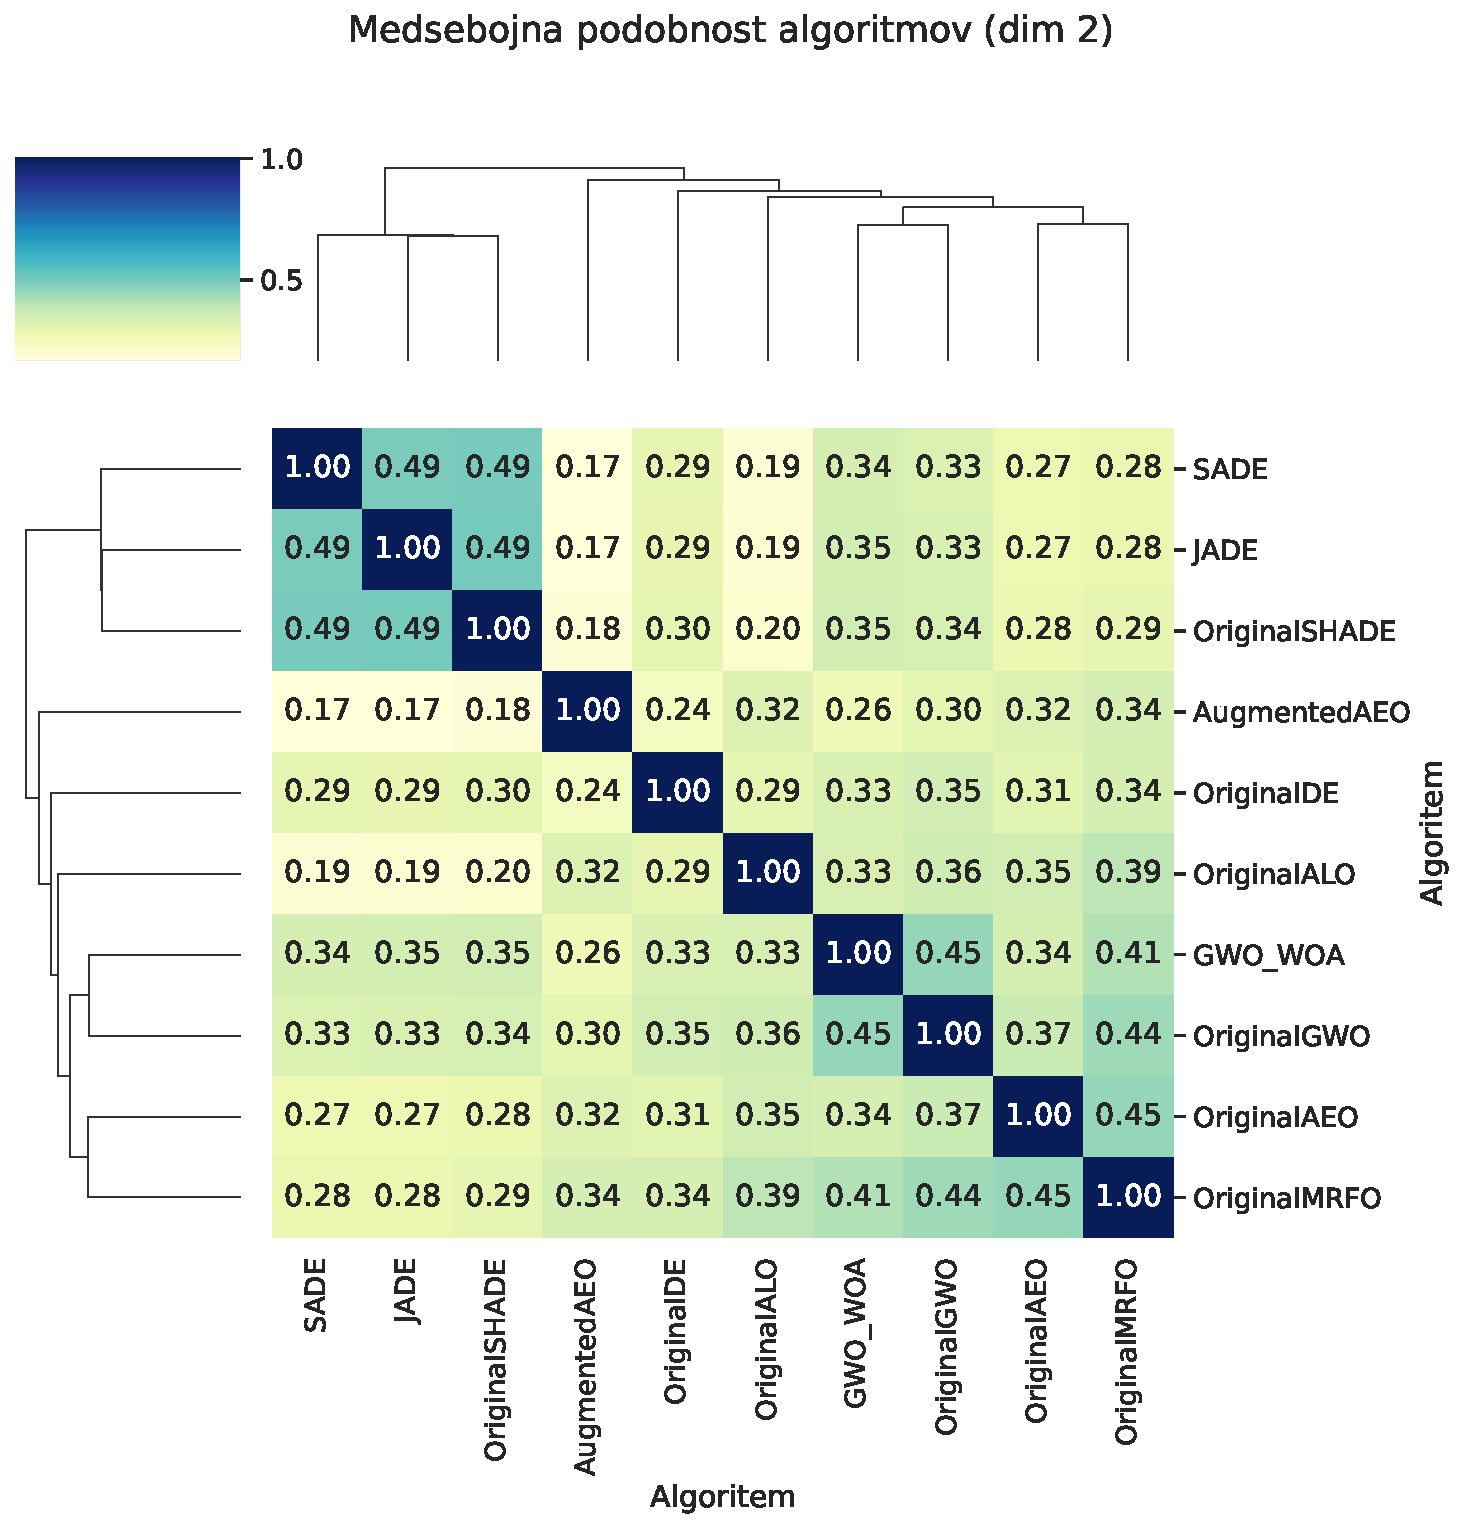
\includegraphics[width=0.75\textwidth]{Slike/Diploma_slike/algorithm_mean_similarity_clustermap_dim_2_scale_False.pdf}
    \caption{Gručenje algoritmov na podlagi kosinusne podobnosti, dimenzija
    2.}
    \label{fig:grucenje-kosinusna}
\end{figure}
Slika~\ref{fig:grucenje-raziskovanje} nazadnje prikazuje gručenje na podlagi
razlike v raziskovanju (razdelek~\ref{sec:exploration}) na problemu
$\prob{23}{1}$ pri dimenziji 5. Tudi tu se družina DE (SADE, OriginalDE,
OriginalSHADE) tesno združi (medsebojne razlike $5{,}1$--$8{,}9$), medtem ko
AugmentedAEO in OriginalALO ostaneta vedenjska osamelca z visokimi razlikami
do skoraj vseh preostalih algoritmov.
\begin{figure}[H]
    \centering
    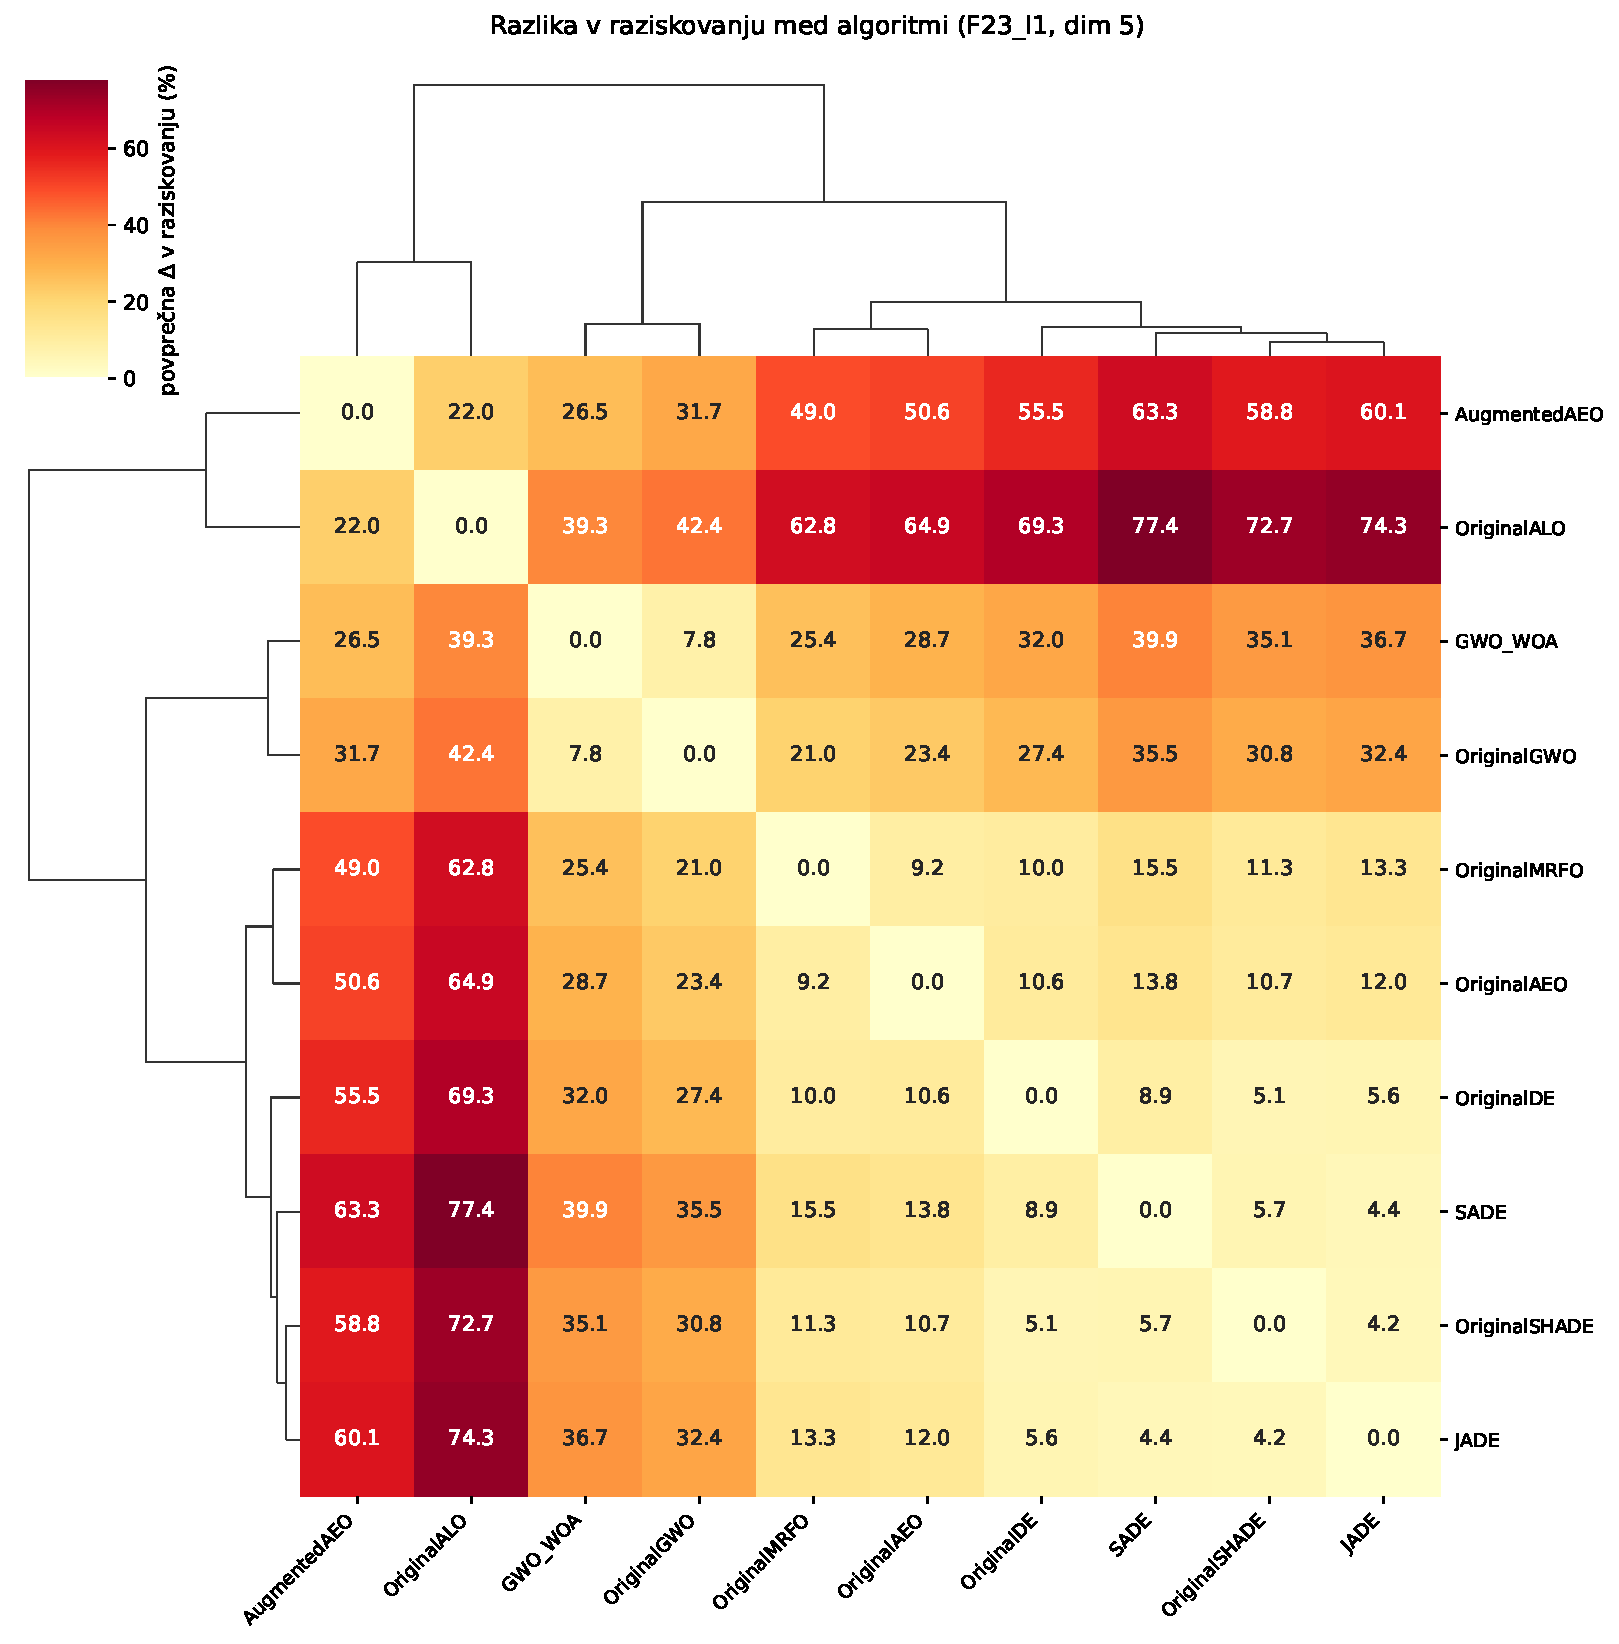
\includegraphics[width=0.85\textwidth]{Slike/Diploma_slike/exploration_difference_clustermap_F23_I1_dim5.pdf}
    \caption{Gručenje algoritmov na podlagi razlike v raziskovanju, problem
    $\prob{23}{1}$, dimenzija 5.}
    \label{fig:grucenje-raziskovanje}
\end{figure}
Družina DE se tako gruči skupaj v vseh treh, med seboj neodvisnih merah.
Prav tako drži za oba algoritma iz GWO družine (GWO\_WOA in OriginalGWO), ki
se prav tako dosledno združita v vseh treh. Njuna medsebojna podobnost
(oziroma razlika) je vsakič med najvišjimi (oziroma najnižjimi) v celotni
matriki, primerljivo z družino DE. Kar je še bolj zanimivo, je to, da se na
videz nepovezana algoritma, OriginalAEO in OriginalMRFO, prav tako združita v vseh treh clustermapih. To nakazuje na precejšnjo
vedenjsko podobnost med njima, ki je iz samih imen ali izvora algoritmov ne
bi pričakovali.

\section{Dodana vrednost mer}
\label{sec:dodana-vrednost}

Kosinusna razdalja iz razdelka~\ref{sec:cosine} je edina mera, ki jo v tem
delu prevzamemo iz predhodnega dela. Smiselno je torej vprašanje, kaj
preostalih pet mer sploh prispeva. Da to preverimo, izberemo štiri pare
algoritmov: dva, ki sta si po kosinusni razdalji zelo podobna, in dva, ki
sta si po njej različna. Za vsakega prikažemo vrednosti vseh šestih mer na
ločljivi, unimodalni funkciji $F_1$, na multimodalni funkciji s šibko
globalno strukturo $F_{23}$ ter povprečje čez vse obravnavane probleme
(slika~\ref{fig:dodana-vrednost}).

\begin{figure}[p]
    \centering
    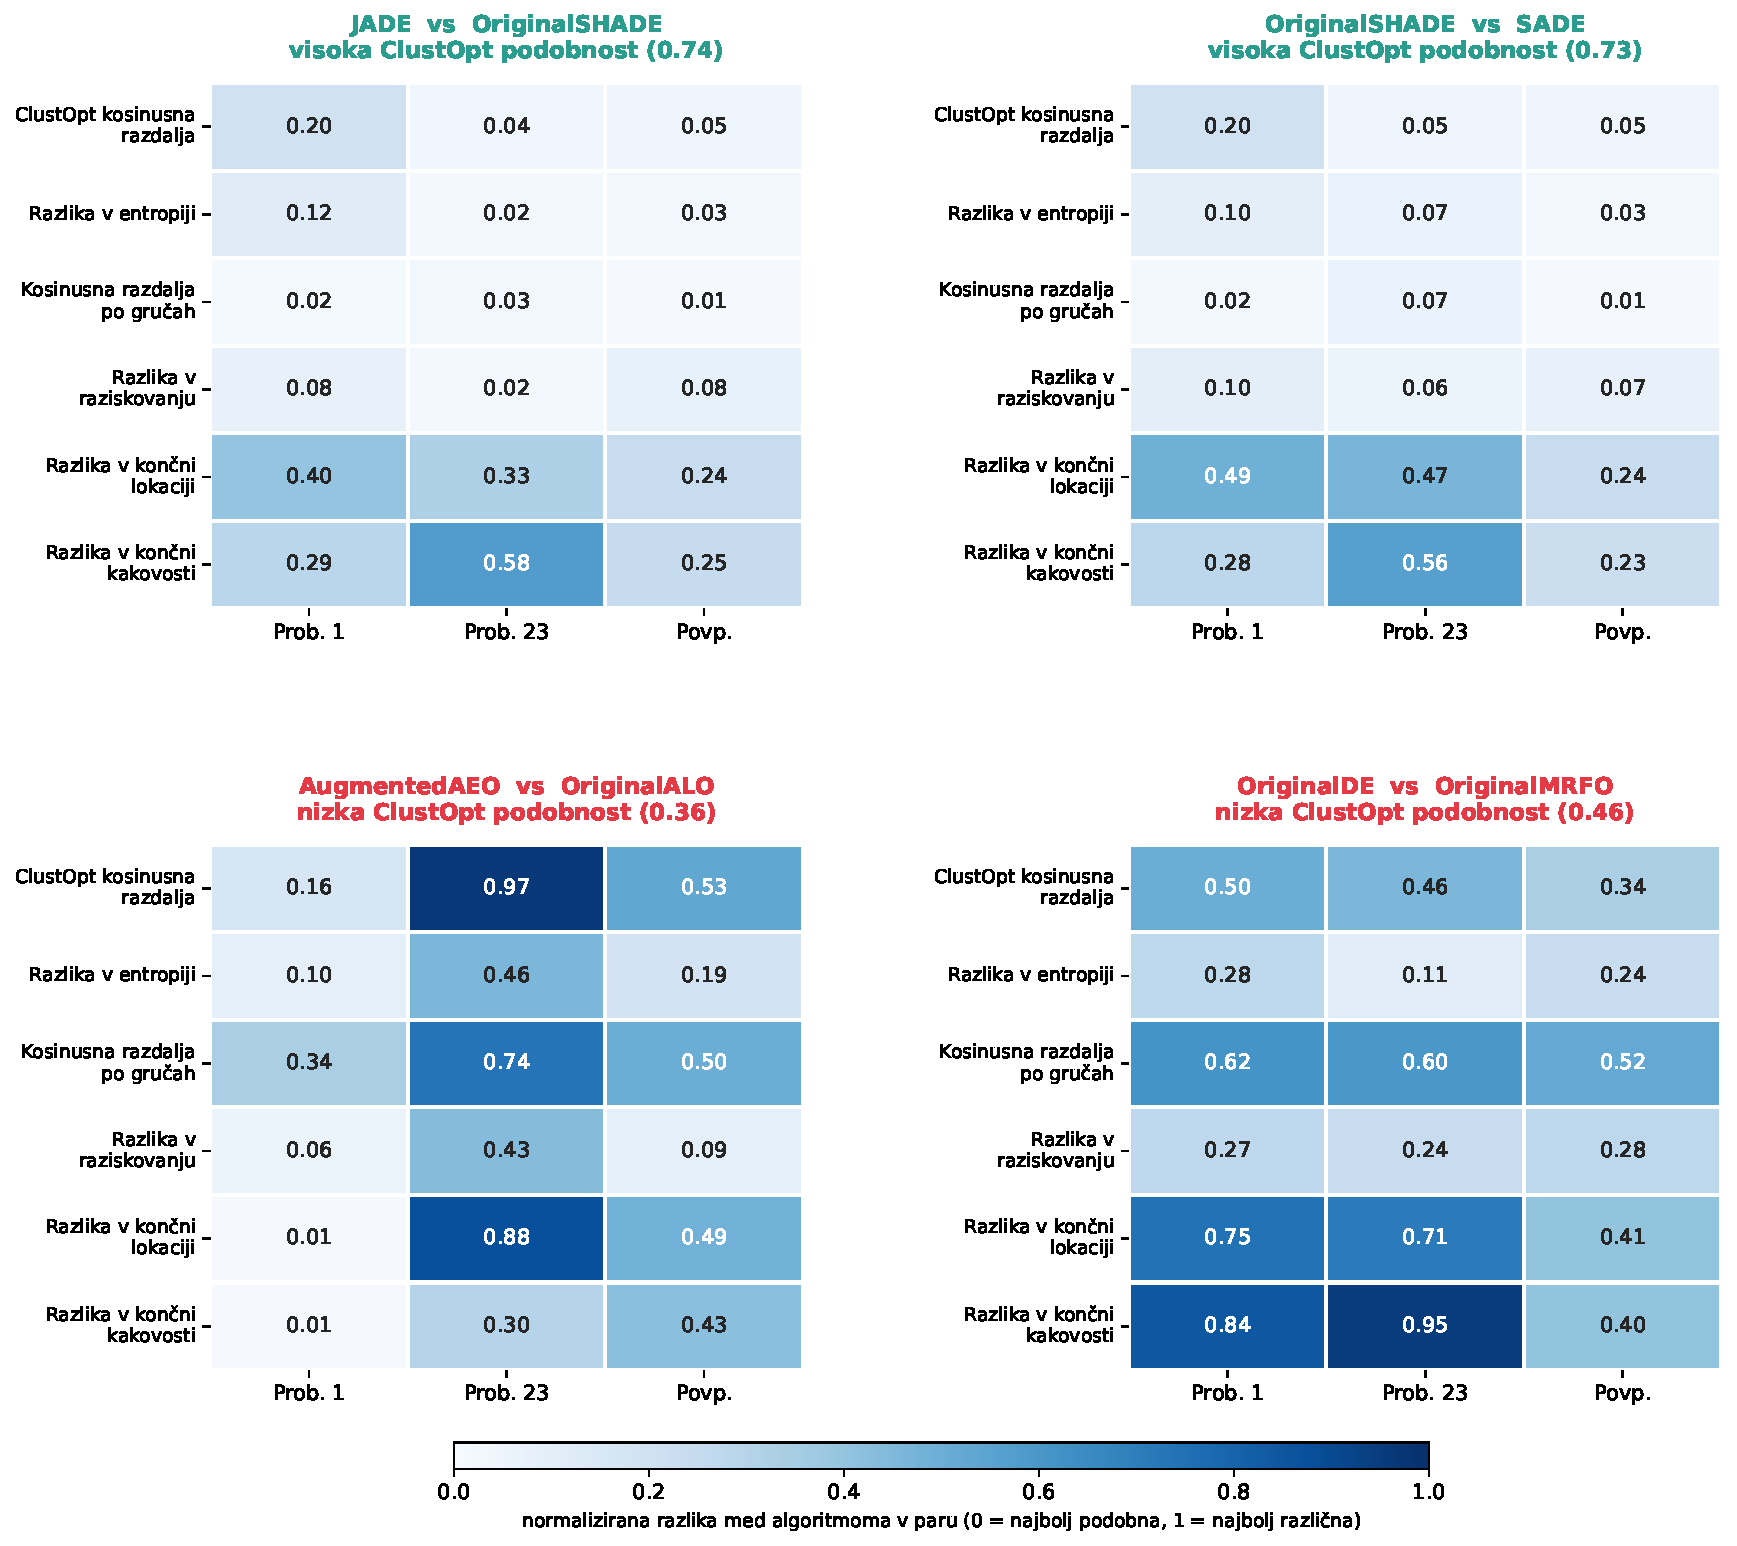
\includegraphics[width=\textwidth]{Slike/Diploma_slike/dodana_vrednost_mer_dim2.pdf}
    \caption{Vrednosti šestih mer za štiri pare algoritmov, dimenzija 2.
    Vrednosti so percentilni rangi znotraj posameznega problema, izračunani
    čez vseh $\binom{28}{2} = 378$ parov. Celica torej pove, kje je par
    glede na razpon vseh parov na tem problemu. To je storjeno zaradi potencialno neomejenih vrednosti razlike v lokaciji in fitnesu. Oznaki \emph{visoka} in
    \emph{nizka} podobnost sta relativni glede na obravnavani nabor.}
    \label{fig:dodana-vrednost}
\end{figure}

Pri paru JADE in OriginalSHADE kosinusna razdalja na problemu $F_{23}$ znaša
$0{,}04$, torej sta si po njej med najbolj podobnimi pari v naboru, razlika v
končnem fitnessu pa hkrati $0{,}58$. Podobno velja za par OriginalSHADE in
SADE, kjer kosinusna razdalja znaša $0{,}05$, razlika v končnem fitnessu $0{,}56$ in
razlika v končni lokaciji $0{,}47$. Vzorec se ohrani tudi v povprečju čez vse
probleme, kjer je pri obeh parih kosinusna razdalja $0{,}05$, razliki v
lokaciji in fitnessu pa okoli $0{,}24$. Podobna trajektorija skozi gruče
torej ne pomeni \emph{nujno} niti primerljivo dobre rešitve niti
primerljivega mesta v iskalnem prostoru.

Obratna smer je razvidna pri paru AugmentedAEO in OriginalALO. Njegova
povprečna kosinusna razdalja znaša $0{,}53$, medtem ko razlika v entropiji
znaša $0{,}19$ in razlika v raziskovanju le $0{,}09$. Kosinusna razdalja ju
torej uvrsti med bolj različne pare, entropija in raziskovanje pa pokažeta,
da sta si po stopnji razpršenosti populacije precej podobna. Razlog je v tem,
kaj posamezna mera zajame. Kosinusna razdalja je občutljiva na to,
\emph{katere} gruče so zasedene, entropija in raziskovanje pa merita,
\emph{kako razpršena} je populacija. Dva algoritma sta lahko enako razpršena
v povsem različnih delih iskalnega prostora.

Isti par razkrije še tretjo lastnost, in sicer močno odvisnost kosinusne
razdalje od težavnosti problema. Na funkciji $F_1$ znaša $0{,}16$, na
funkciji $F_{23}$ pa $0{,}97$. Po tej meri sta si algoritma torej skoraj
enaka na preprostem in skoraj maksimalno različna na zahtevnem problemu.
Mehanizem za tem razkrijeta sliki~\ref{fig:trajektorije-f1}
in~\ref{fig:trajektorije-f23}, ki prikazujeta zasedenost gruč skozi
iteracije za oba algoritma na obeh problemih. Na funkciji $F_1$ oba
algoritma populacijo v celoti skoncentrirata v \emph{isto} gručo, tisto s
središčem v $(0{,}26, -1{,}16)$. OriginalALO to doseže v šesti,
AugmentedAEO pa v enajsti iteraciji. Ker zasedata isto regijo, so nizke tudi
vse preostale mere. 

\begin{figure}[H]
    \centering
    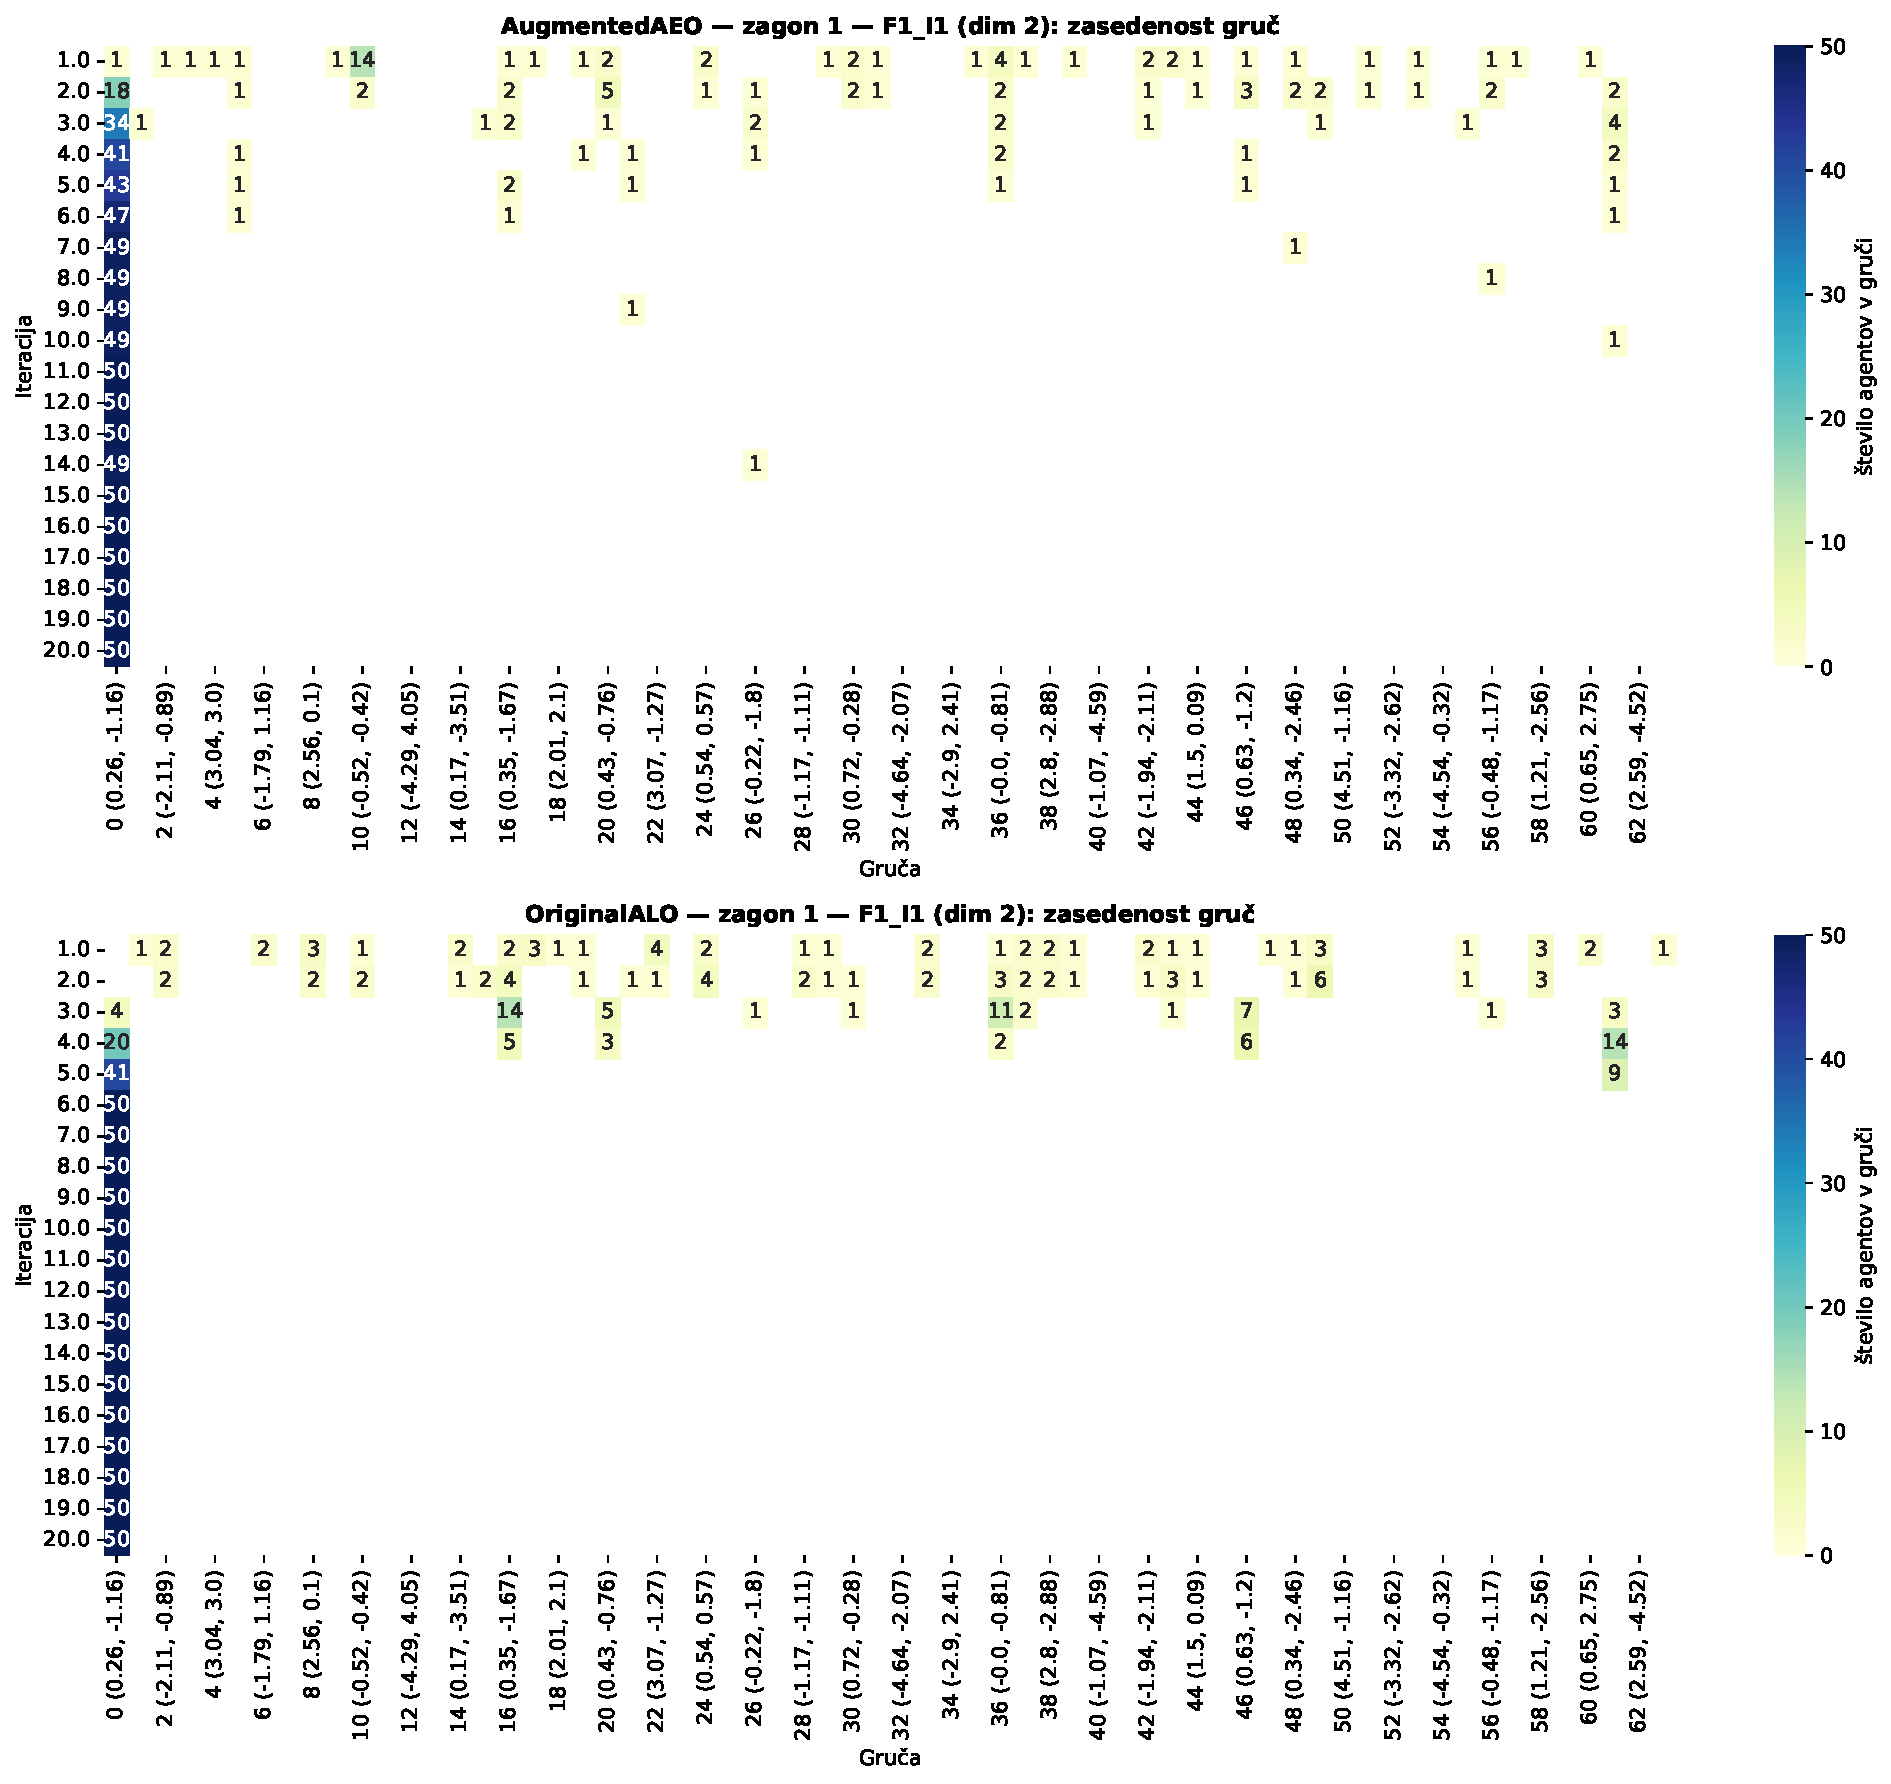
\includegraphics[width=\textwidth]{Slike/Diploma_slike/clustering_latest_F1_I1_AugmentedAEO+OriginalALO_run_1_dim_2.pdf}
    \caption{Zasedenost gruč skozi iteracije za algoritma AugmentedAEO in
    OriginalALO na problemu $F_1I_1$ (dimenzija 2, zagon 1). Oba populacijo
    skoncentrirata v isto gručo.}
    \label{fig:trajektorije-f1}
\end{figure}

Na funkciji $F_{23}$ je slika povsem drugačna. AugmentedAEO se usmeri v
gručo s središčem v $(-0{,}36, 4{,}60)$, OriginalALO pa v gručo s središčem
v $(0{,}09, -2{,}71)$. Prav zato kosinusna razdalja doseže $0{,}97$, razlika v končni
lokaciji pa $0{,}88$. Razlika v končnem fitnessu je hkrati le $0{,}30$, kar
je značilno za multimodalne krajine. Algoritma najdeta različna bazena
primerljive kakovosti. Razliki v entropiji ($0{,}46$) in raziskovanju
($0{,}43$) sta zmerni, saj OriginalALO populacijo zbere popolnoma, medtem ko
AugmentedAEO ohrani nekaj agentov razpršenih po preostalih gručah.

\begin{figure}[H]
    \centering
    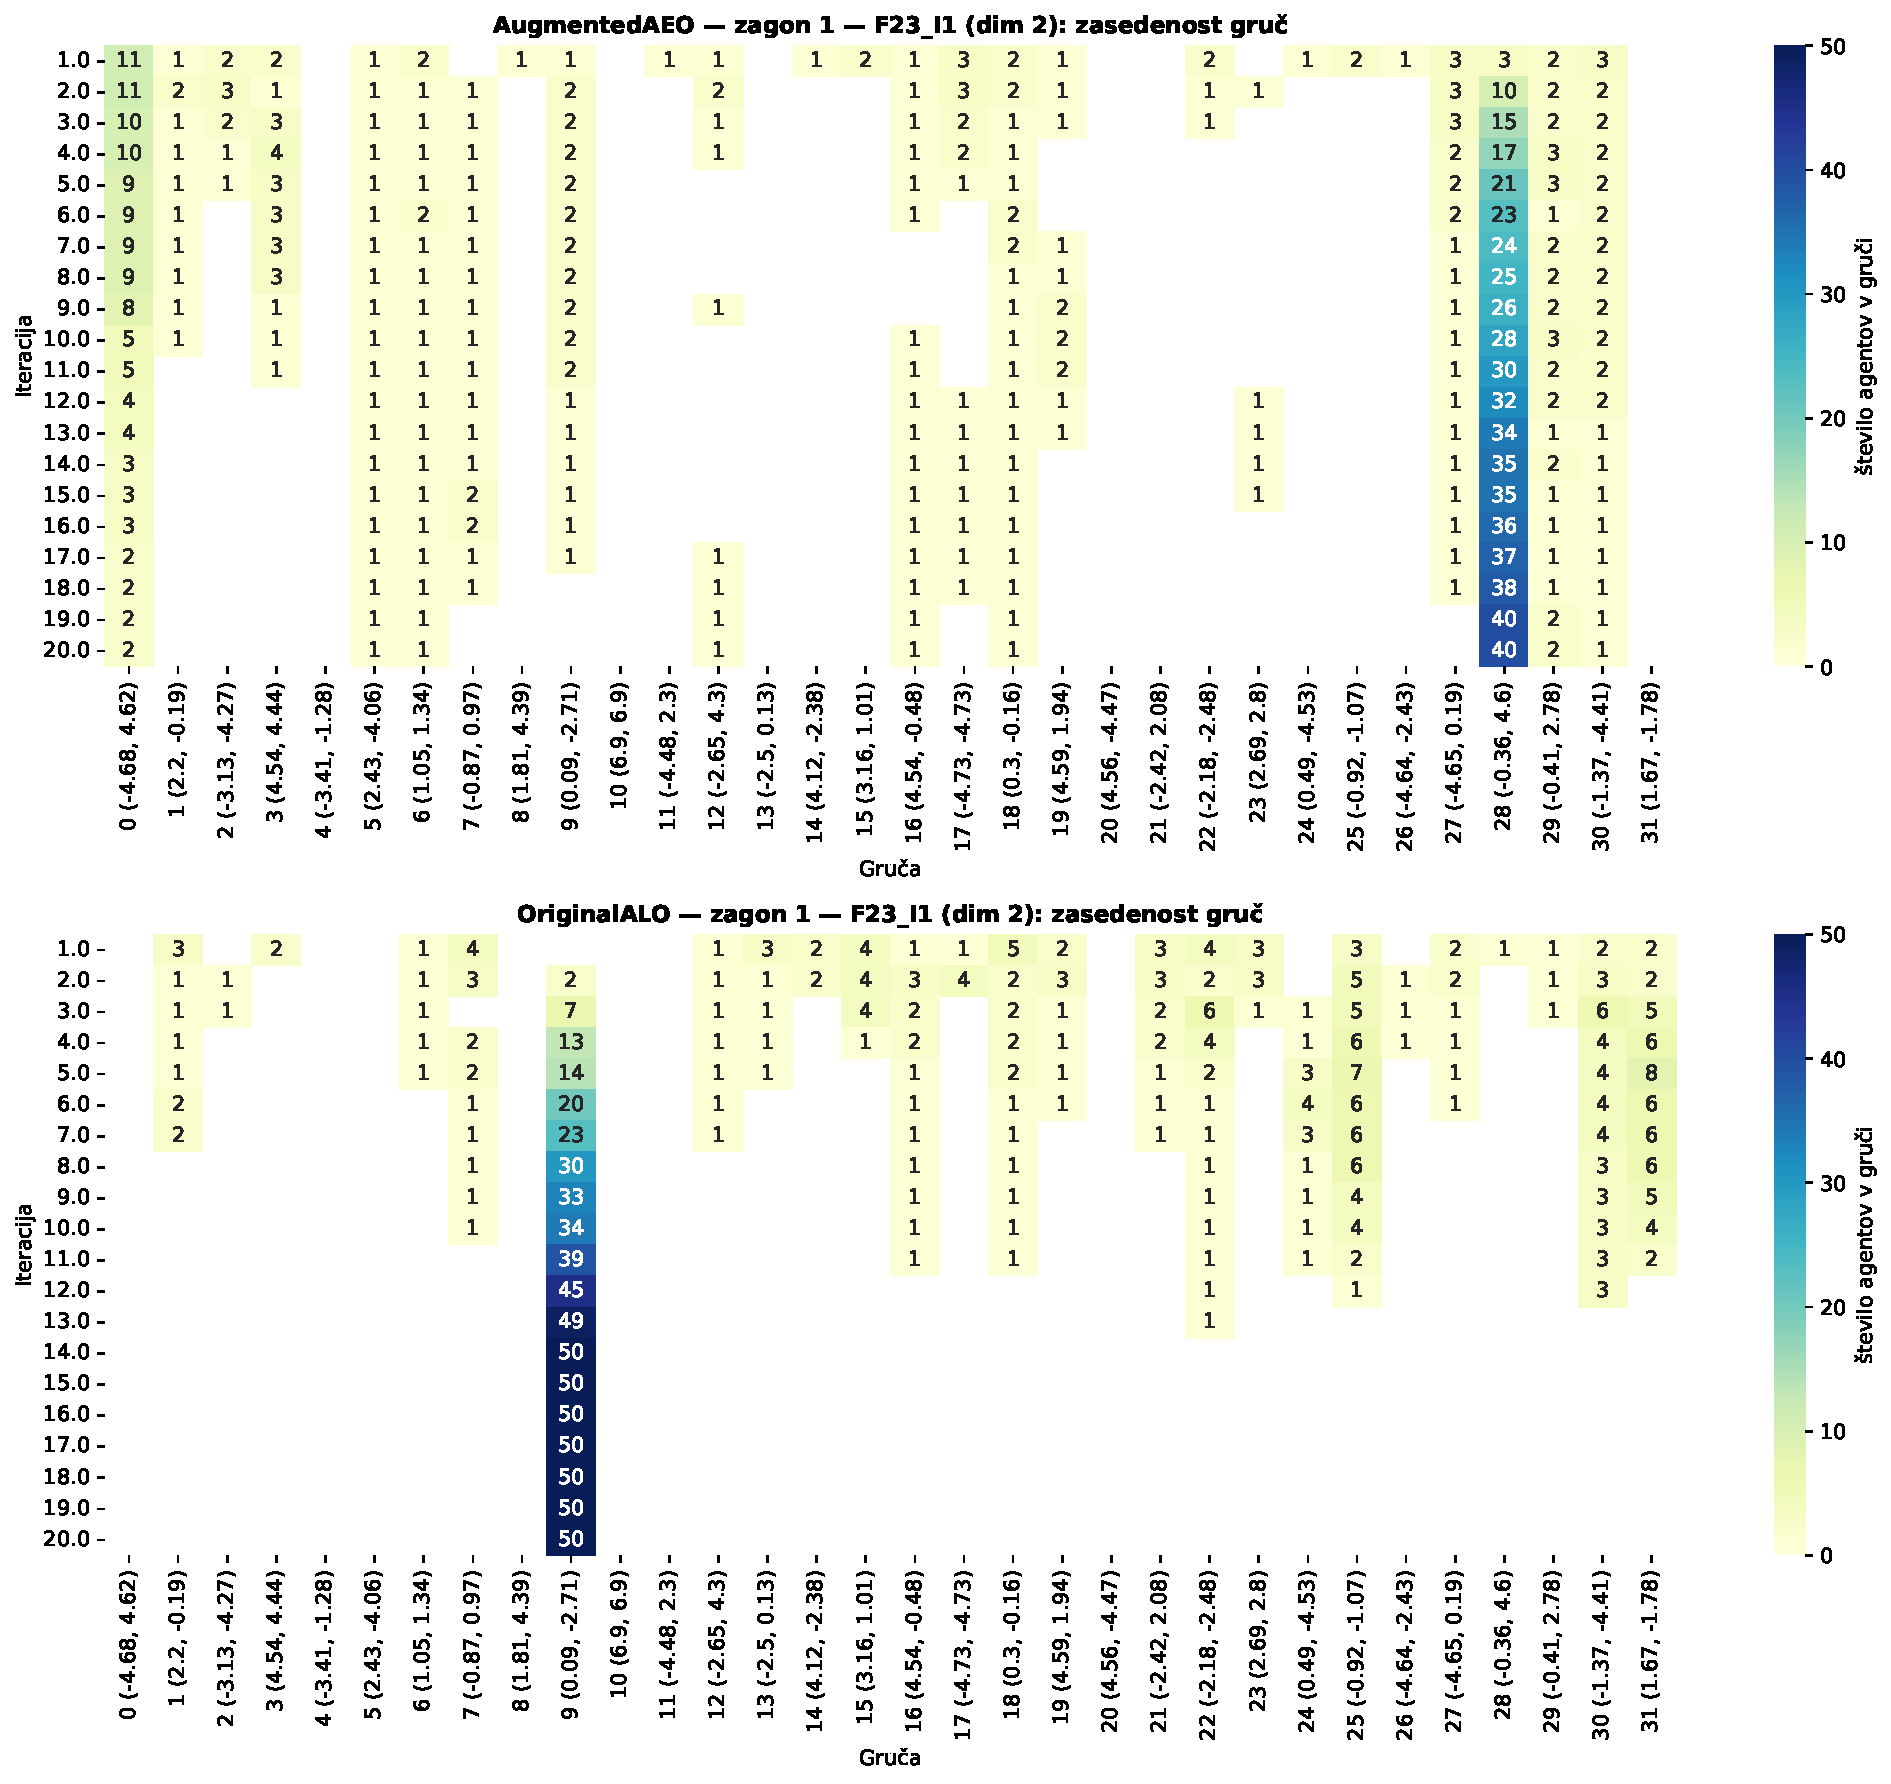
\includegraphics[width=\textwidth]{Slike/Diploma_slike/clustering_latest_F23_I1_AugmentedAEO+OriginalALO_run_1_dim_2.pdf}
    \caption{Zasedenost gruč skozi iteracije za algoritma AugmentedAEO in
    OriginalALO na problemu $F_{23}I_1$ (dimenzija 2, zagon 1). Algoritma se
    usmerita v različni gruči, kar pojasni visoko kosinusno razdaljo kljub
    zmerni razliki v entropiji.}
    \label{fig:trajektorije-f23}
\end{figure}


\chapter{Zaključek}
\label{ch:zakljuck}

Predstavili smo nabor šestih komplementarnih mer, ki
vedenje dveh metahevrističnih algoritmov primerjajo iz njunih iskalnih
trajektorij in ne le iz končne rešitve. Pet mer je izvirnih,
kosinusno razdaljo in postopek gručenja smo prevzeli iz predhodnega
dela~\cite{clustopt2025}.

Analiza na 28 algoritmih je pokazala naslednje. Mere se med seboj večinoma ne
podvajajo, saj tudi tiste iz istega vira korelirajo le zmerno
(razdelek~\ref{sec:spearman}). Edini par z visoko korelacijo, entropija in
razlika v raziskovanju, izhaja iz neodvisnih virov in ga zato beremo kot
konvergentno veljavnost
(razdelek~\ref{sec:konvergenca}). Povezava med razliko v lokaciji in
razliko v fitnessu z naraščajočo dimenzijo slabi, kar podpira
izhodiščno tezo, da končni rezultat sam ne opiše iskalnega vedenja
(razdelek~\ref{sec:dimenzije}). Isto se na ravni posameznih algoritmov
pokaže na problemu $F_{21}$ (razdelek~\ref{sec:entropija-fitness}). Mere
kljub medsebojni neodvisnosti prepoznajo iste vedenjske družine
(razdelek~\ref{sec:grucenje-metrike}).

Delo ima omejitve. Obe kosinusni meri sta neobčutljivi na magnitudo, mera
razlike v lokaciji pa je primerljiva le znotraj instance. Ugotovitve
veljajo za obravnavani nabor 28 algoritmov in jih ne posplošujemo na
metahevristike nasploh. Služijo naj kot ilustracija uporabe mer in primerjav algoritmov.

Časovno togost kosinusnih mer bi lahko odpravili z dinamičnim časovnim
prilagajanjem (angl. dynamic time warping - DTW), neobčutljivost na magnitudo z uteženo različico, vrstni red
obiskovanja gruč pa z Markovskimi prehodnimi matrikami, nabor sam pa
preizkusili na več algoritmih in v višjih dimenzijah.


\newpage
\ \\
\clearpage
\addcontentsline{toc}{chapter}{Literatura}
\bibliographystyle{plain}
\bibliography{literatura}


\end{document}